\documentclass{gatech-thesis}
% The default options:
%   \documentclass[11pt,letterpaper,oneside,%
%       doublespaced,normalmargins,final]{gatech-thesis}
% will generate a document that conforms to the graduate studies office
% guidelines.

\ifx\pdfoutput\undefined
  \usepackage[dvips,final]{graphicx}  % using latex+dvips
  \usepackage[dvips,usenames]{color}
\else
  \usepackage[pdftex,final]{graphicx} % using pdflatex
  \usepackage[pdftex,usenames]{color}
\fi

% this is for URL pretty-printing
\usepackage{url,comment,multirow,algorithm,algorithmic}

% this is for including code listings
\usepackage{listings}
\lstset{
  language=C,	
  basicstyle=\small,
  keywordstyle=\color{black},
  identifierstyle=,
  commentstyle=\color{red},
  stringstyle=\ttfamily,
  showstringspaces=false,
  framerule=0.5mm,
}

\usepackage{tikz}
\usepackage{textcomp}
\usepackage{boxedminipage, amsmath,algorithm, algorithmic}
\usepackage{amssymb}

\graphicspath{{figures/}}

%
% TITLE BUZZWORDS: discriminate, differentiated, individualized,
% personalized, distinguished, divergent
%

%define stuff in preamble
 \degree{Doctor of Philosophy}
 \department{College of Computing}
% alternative names: Melange / Farrago / Pasticcio
 \title{System Design Principles for Heterogeneous Resource Management and Scheduling in Accelerator-Based Systems
}
%\title{System Support for Enterprise-Wide Performance Management}
 \author{Dipanjan Sengupta}
 \principaladvisor{Prof. Karsten Schwan}
 \committeechair{Dr. Matthew Wolf}
 \firstreader{Dr. Ada Gavrilovska}
 \secondreader{Prof. Ling Liu}
 \thirdreader{Prof. Sudhakar Yalamanchili }
 \fourthreader{Prof. Richard Vuduc}
 \fifthreader{Dr. Theodore L. Willke}
 \submitdate{16 May 2016}

 \copyrightyear{2016} %add one if thesis submitted in Dec.

\thesisproposalfalse       % default
 \copyrighttrue  
% \thesisproposaltrue
% \titlepagetrue             % default
% \signaturepagetrue         % default
% \copyrightfalse            % default
% \figurespagetrue           % default
 % \figurespagefalse          % for now...
% \tablespagetrue            % default
  %\tablespagefalse           % for now...
  %\contentspagetrue          % default
% \dedicationheadingfalse    % default
% \bibpagetrue               % default
  \bibpagetrue               % default
% \strictmarginstrue         % default

\bibfiles{ref}

\begin{document}
\bibliographystyle{gatech-thesis}
\setchaptertocdepth{2}

\begin{preliminary}
\begin{dedication}
\null\vfil
{\Large
\begin{center}
To my parents.
\end{center}}
\vfil\null
\end{dedication}

\begin{acknowledgements}
First and foremost I would like to express my special appreciation and thanks to my advisor Prof. Karsten Schwan. It has been an honor to be his Ph.D. student. He has inspired me greatly to work in high performance computing (HPC) field. His willingness to motivate me and to help me grow as a researcher has contributed greatly to this thesis work. I am absolutely indebted to all his contributions of time, ideas, and research directions making my Ph.D. experience the most intellectually stimulating and enjoyable time in my career so far. I would also like to thank Dr. Matthew Wolf, Dr. Ada Gavrilovska and Dr. Jeffrey Young for mentoring and advising me at various points in my research. 

I would like to thank the other members of my dissertation committee, Prof. Sudhakar Yalamanchili, Prof. Ling Liu and Dr. Theodore L. Willke for serving as my committee members and for their insightful comments and suggestions on my research. My mentors during my internships at Intel Labs, Xia Zhu (Ivy) and Narayanan Sundaram, have had a major impact on shaping the ideas presented in this thesis. I would also like to express my special thanks to my manager at Intel Labs Theodore L. Willke, who is still a mentor to me. Susie McClain, our group admin, who has been extremely helpful in taking care of our travels, day to day lab needs, etc deserves a special approbation. Not many people can keep that amount of organization and detail in their head.

My time at Georgia Tech  was made enjoyable in large part due to many friends and groups that became a part of my life. I am grateful for the time spent and several intellectually stimulating discussions with my past and present labmates in the CERCS group over the years. A special mention to Minsung Jang, Ketan Bhardwaj, Bharath Srinivasan, Mukil Kesavan, Abhinav Narain, Sudarsun Kannan, Hrishikesh Amur, Vishal Gupta, Subramanya R. Dulloor, Min Lee, Fang Zheng, Hobin Yoon, Alex Merritt, Junwei Li and Jai Dayal. Mukil and Minsung were particularly very helpful in giving me general advice for a successful Ph.D. life. I hope to keep in touch with all of them in future. I am extremely grateful to Sudarsun for being the nicest roommate ever. I have learnt so much from him and he always has the most sound advice I can get on life issues. I would also like to thank all my friends from IIT Kharagpur: Subhra Mazumdar, Puneet Jain, Satya Gautam, Pranith Kumar, Karan Doshi and Anchal Nema for helping me feel lighthearted during the most stressful moments in my Ph.D. life. 

Finally, I would like to thank my family for their love and support, without whom I would have given up a long time ago. For my parents who have always supported me in all my pursuit be it my interest in higher studies or my love for liberal arts. For the presence of my elder brother one phone call away with his intellectually and spiritually stimulating advice. I would like to dedicate this thesis to my parents for what I am today is all because of them.	

\end{acknowledgements}
\contents
%\begin{abstract}
Accelerator-based systems are making rapid inroads into becoming platforms of choice for both high end cloud services and processing irregular applications like real-world graph analytics due to their high scalability and low dollar to FLOPS ratios. Yet GPUs are not first class schedulable entities causing substantial hardware resource underutilization, including their computational and data movement engines. Therefore, software solutions with support for efficient resource management principles are required to address such scheduling crisis in GPUs. Further, two important characteristics of real world graphs like those in social networks are that they are big and are constantly evolving over time. This poses challenge due to limitations in GPU-resident memory for storing these large graphs. And because of the high rate at which these large-scale graphs evolve, it is undesirable and computationally infeasible to repeatedly run static graph analytics on a sequence of versions, or snapshots, of the evolving graph. 
Therefore, novel incremental solutions are required to process large-scale evolving graphs in near real-time using GPUs with memory footprint exceeding the device's internal memory capacity. 

First, the thesis proposes Strings, a GPU scheduling infrastructure  that achieves high system throughput and fairness among applications from multiple tenants using manycore GPU servers by treating GPUs as  first class schedulable entities, and decomposing the scheduling problem into a novel combination of load balancing and per-device resource sharing.

Second, for processing graph applications with larger memory footprint than the device memory the thesis proposes GraphReduce, a highly efficient and scalable GPU-based framework that adopts a combination of edge- and vertex-centric implementations of the Gather-Apply-Scatter programming model and operates on multiple asynchronous GPU streams to fully exploit the high degrees of parallelism in GPUs supporting efficient graph data movement between the host and device. Finally the thesis also proposes a novel programming model that allows for implementing a large set of incremental graph processing algorithms seamlessly across multiple GPU cores. It also characterizes various graph algorithms and how related graph properties affect the complexity of incremental graph processing in making runtime decisions to choose between an incremental vs static run over a particular update batch to achieve the best performance.
\end{abstract}


\begin{summary}
Accelerator-based systems are making rapid inroads into becoming platforms of choice for both high-end cloud services and processing applications with irregular access pattern such as real-world graph analytics, due to their high scalability and low dollar to FLOPS ratios. Yet GPUs are not first class schedulable entities causing substantial hardware resource underutilization, including their computational and data movement engines. Therefore, software solutions with support for efficient resource management principles are required to address such scheduling crisis in GPUs. Further, two important characteristics of real world graphs like those in social networks are that they are big and are constantly evolving over time. This poses challenge due to limitations in GPU-resident memory for storing these large graphs. And because of the high rate at which these large-scale graphs evolve, it is undesirable and computationally infeasible to repeatedly run static graph analytics on a sequence of versions, or snapshots, of the evolving graph. 
Therefore, novel incremental solutions are required to process large-scale evolving graphs in near real-time using GPUs with memory footprint exceeding the device's internal memory capacity. 

First, to address the challenges of GPU multi-tenancy, the thesis presents \textit{Strings} scheduler for heterogeneous manycore nodes that implements a model in which GPUs are treated as first class schedulable entities, by decomposing the scheduling problem into a combination of load balancing and per-device resource sharing. Its utility as an infrastructure for developing and evaluating advanced scheduling methods is demonstrated for server workloads, where (i) load balancing intelligently binds each application’s GPU component to an appropriate GPU and, (ii) device-level sharing aims to keep all of a GPU’s hardware units busy, by concurrently running those applications that reside in different phases of their use of the GPU. It also prioritizes GPU requests that have attained `least service' to achieve high system throughput, and goes beyond that to also ensure fairness via a history based fair-share scheduler. Over a wide variety of multi-tenant workloads, Strings achieves substantial speedups compared to that obtained by the native CUDA runtime and other competitive GPU schedulers. 

Second, to address the problem of processing graph applications with larger memory footprint than the device memory the thesis presents \textit{GraphReduce}, a highly efficient and scalable GPU-based framework that adopts a combination of edge- and vertex-centric implementations of the Gather-Apply-Scatter programming model and operates on multiple asynchronous GPU streams to fully exploit the high degrees of parallelism in GPUs supporting efficient graph data movement between the host and device. GraphReduce (GR) runs graph algorithms on GPUs without unduly burdening graph algorithm developers. Programmers write the appropriate sequential codes for their graph algorithms and then use its simple APIs to express their use for processing various graphs. The GR runtime seamlessly partitions the graph into different shards, each single one of which entirely fits into GPU memory, and overlaps shard movement with GPU-level graph processing, the latter using multiple levels of GPU-level parallelism. With such automation, GR can deal with graph sizes much exceeding GPU memory sizes. Extensive experimental evaluations for a wide variety of graph inputs and algorithms demonstrate that GraphReduce significantly outperforms other competing out-of-memory approaches.


Finally, we address the problem of processing real-world graphs that are constantly evolving over time using GPUs. Although modern GPUs provide massive amount of parallelism for efficient graph processing, the challenges remain due to their lack of support for this near real-time streaming nature of dynamic graphs. Specifically, because of the current high volume and velocity of graph data combined with the complexity of user queries, traditional processing methods by first storing the updates and then repeatedly running static graph analytics on a sequence of versions or snapshots are deemed undesirable and computational infeasible on GPU. To address this problem of analyzing evolving graphs in near real- time, we present \textit{EvoGraph}, a highly efficient and scalable GPU-based dynamic graph analytics framework that incrementally processes graphs on-the-fly using fixed-sized batches of updates. To realize this vision, we propose a novel programming model called I-GAS that is based on the gather-apply-scatter programming paradigm and that allows for implementing a large set of incremental graph processing algorithms seamlessly across multiple GPU cores. Further we propose novel optimizations like property-based dual path execution in the EvoGraph framework to choose between an incremental vs static run over a particular update batch and GPU 'context merging' to efficiently use of all hardware resources using GPU streams, including its computational and data movement engines. Extensive experimental evaluations for a wide variety of graph inputs and algorithms demonstrate that EvoGraph achieves substantial speedup compared to static graph recomputation and other competing streaming graph processing frameworks such as STINGER.

\end{summary}
\end{preliminary}

\chapter{Introduction}
\label{intro}

High performance machines are increasingly using GPUs~\cite{15, 16, 17, 18, 19}, to leverage their scalability and low dollar to FLOPS ratios.  As a result, GPUs have become the main compute engines for today’s HPC clusters and supercomputers like the Titan supercomputer in Oak Ridge~\cite{titan}. This trend continues with the move toward exascale machines~\cite{exascale1, exascale2, exascale3, exascale4, exascale5, exascale6, exascale7}, with compute nodes expected to be comprised of millions of accelerator and general purpose cores, whether packaged as `thin' or `fat' nodes (shown in Figure~\ref{fig:hybrid}).  Therefore, it is not only important to efficiently schedule applications to keep all the available cores busy but also  intelligently move the appropriate data near the computation as these accelerators have limited amount of memory attached to them. Existing software infrastructures deal very poorly in terms of scheduling and fine grain resource management of such heterogeneous architecture leading to substantial underutilization of all the available resources, including both the computational and data movement engines. Next we describe three broad classes of applications where there is substantial GPU underutilization and showcase the current scheduling crisis in them. 

\begin{figure}[h]
\begin{center}
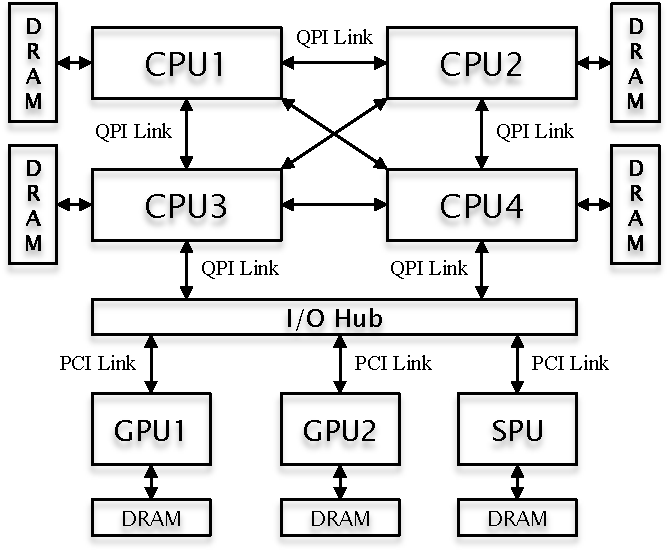
\includegraphics[width=0.70\textwidth]{hybrid}
\caption{Accelerator-based heterogeneous system architecture }
\label{fig:hybrid}
\end{center}	
\end{figure}

\begin{figure}[t]
\begin{center}
\includegraphics[width=0.70\textwidth]{servicemodel}
\caption{GPGPU application service model following a negative exponential
distribution of request arrival from multiple end users. }
\label{fig:service}
\end{center}	
\end{figure}

\section{GPU Sharing in Cloud}
A recent trend is the gain in popularity of computationally intensive high performance applications in client-server workloads including image processing algorithms like video transcoding~\cite{element} , financial algorithms~\cite{zillians}, online gaming, e.g., NVIDIA’s cloud gaming~\cite{nvidia-game}, search~\cite{GPUsearch}, data mining~\cite{GPUmine} and multimedia services like Adobe’s Photoshop.com~\cite{adobe}. This motivates online services to take advantages of GPU clusters. This is mirrored by GPU offerings by cloud providers like Amazon ECC~\cite{amazon}, Nimbix~\cite{nimbix}, Peer1 Hosting~\cite{peer1}, and Penguin Computing~\cite{penguin}.  Figure~\ref{fig:service} shows the application service model for a multi-tenant single GPU server.

A challenge to using GPUs in these multi-tenant server and cloud environment is the lack of sophisticated support for GPU scheduling, given the predominant model of treating GPUs as statically chosen devices, in which applications explicitly and programmatically select the GPU devices on which they wish to run, rather than as first class schedulable entities~\cite{pegasus}. Such static GPU assignments will inhibit concurrency, particularly with the varying workloads imposed by web applications. For instance, during peak demands for certain services, some GPU devices will be heavily utilized while other services’ GPUs will be idle or underutilized. Low GPU utilization can also be attributed to considerable diversity in the fraction of CPU vs. GPU component in applications, for reasons that include an inability to parallelize certain application components and/or limited GPU residency vs. the costs of host-GPU data transfers. Finally, although each GPU can internally contain thousands of cores, it is treated by applications as a single SIMD engine, potentially resulting in the serial execution of GPU contexts that could have been executed concurrently.

\section{Large-Scale Graph Analytics on GPUs}
With the increasing interest in many emerging domains such as social networks, the World Wide Web (e-commerce and advertising), and genomics, the importance of graph processing has grown substantially. Some examples of graph analytics include friend/product recommendations, anomaly and trend detection, online advertisement serving etc. This recent trend has given rise to many graph processing frameworks in both distributed, e.g. GraphLab~\cite{graphlab}, PowerGraph~\cite{powergraph},  Pregel~\cite{pregel}; and single machine shared-memory environments, e.g.  Graphchi~\cite{chi}, X-Stream~\cite{xstream}, Ligra~\cite{ligra} etc. This need to rapidly process large graph-structured data has also engendered recent efforts to leverage cost-efficient GPUs for efficient graph analytics. Doing so, however, requires addressing substantial technical challenges, including (1) dealing with the dynamic nature of graph parallelism, (2) coping with constrained on-GPU memory capacity, i.e., to process graphs with memory footprints that exceed that capacity, and (3) addressing programmability issues for developers with limited insights into how to best exploit the resources of evolving and varied GPU architectures.

More precisely, a graph processing framework using GPUs should expose abstractions or simple APIs for the developers to write the appropriate sequential codes for their domain specific algorithms, e.g., for data mining, machine learning, etc to express their use for processing graphs of arbitrary size. The runtime should then seamlessly (i) partition the graphs into smaller chunks each single one of which entirely fits into GPU memory, (ii) efficiently move data between host and device leveraging concurrent GPU operations to obtain fine-grain parallelism that exploits both GPU software and hardware features like CUDA streams and Hyper-Q of Kepler GPUs etc (iii) choosing the most appropriate programming model ( edge- or vertex- centric or a combination of both) to generate device code for efficient GPU-level graph processing, and iv) finally intelligent coordinated scheduling and management of both the data movement and compute engines to achieve optimal performance. With such automation, we can deal with graph sizes much exceeding GPU memory sizes. This is important because even a common Yahoo web-graph comprised of 1.4 billion vertices requires approximately 6.6 GB of memory to store just its vertex values (not even including the edges and their corresponding states).

In summary, the goal is to  design a scale-up graph processing framework on HPC systems with discrete GPUs and high end (i.e., memory-rich) hosts where GPUs can be used to accelerate analytics performed on graphs with billions of edges, operating at speeds much exceeding that of similar operations run on CPUs, and programmed in ways accessible to programmers who are not experts in GPU programming. 

\begin{figure}[t]
\begin{center}
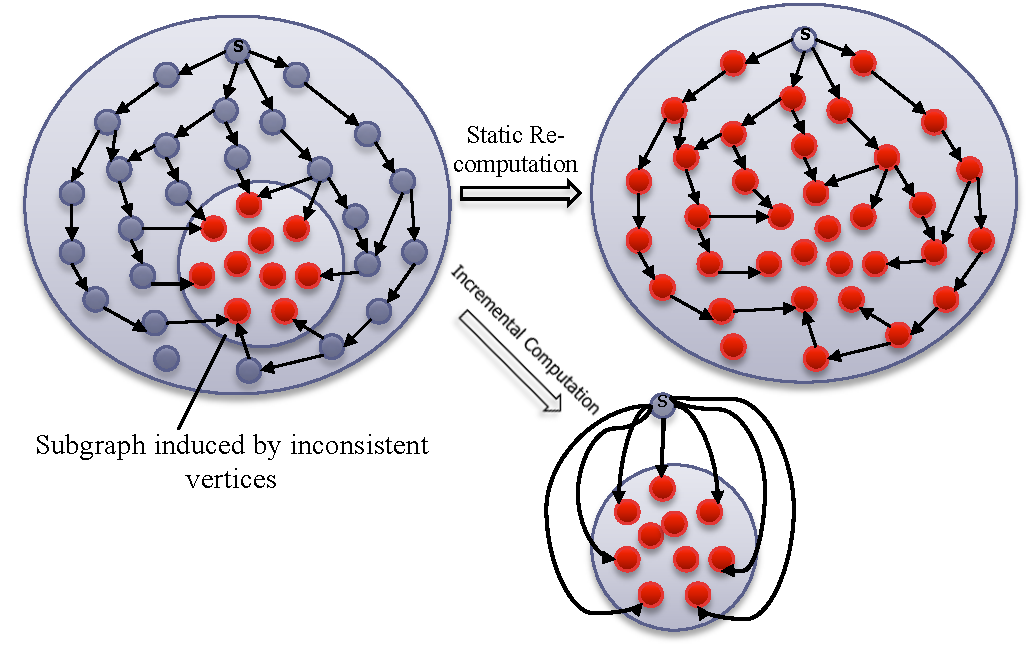
\includegraphics[width=0.70\textwidth]{incremental-graph}
\caption{Static vs. incremental graph processing. }
\label{fig:inc}
\end{center}	
\end{figure}

\section{Dynamic Graph Analytics on GPUs}
Another important aspect of real-world graphs like facebook friend lists or twitter follower graphs is that they dynamically change with time.  Current graph analytics on such dynamic graphs follow a store-and-static-compute model that involves first storing batches of updates to a graph applied at different points in time and then repeatedly running static graph computations on multiple versions or snapshots of this evolving graph sequence. The key assumption made here is that the rate of change in graphs due to continuous updates is slower than the execution time of the static graph analytics. This assumption might not hold true for current real-world graphs. For instance, Twitter traffic can peak at 143 thousand tweets (and associated updates) / per second and emails sent per second can reach as high as 2.5 millions/sec.   Hence, there are two fundamental challenges to applying static recomputation to these types of rapidly changing data sets. First, static graph analytics on a single version of the evolving graph, even when leveraging massive amount of parallelism offered by multiple cores in a high performance cluster, can be very slow due to the extreme scale of many real-world graphs and/or because of the complexity of the graph queries that are traditionally both compute and memory intensive. Therefore, the cumulative cost of analyzing such large-scale versions with complex graph queries repeatedly can be substantially high. Second, there are real world graph analytics problems that inherently require soft or hard real time guarantees, e.g., real-time anomaly detection, disease spreading etc. So to conclude, the current high volume and velocity of graph data combined with the complexity of user queries has outstripped the traditional static graph analytics model on streaming graphs.

To address the above mentioned computational crisis in dynamic graph processing we need a graph processing framework that can incrementally process a continuous stream of updates (i.e., edge/vertex insertions and deletions) as a sequence of batches.  Because the incremental logic, in many practical scenarios, affects only a portion of the graph (as shown in Figure~\ref{fig:inc}), this reduction can result in tremendous performance benefit compared to static recomputation of the graph algorithm on the entire graph for many popular graph algorithms and real-world graphs.
Further, we also need to handle the scenarios when updates to the graph affects a very large portion of the graph and incremental processing won’t help much or may even be worse (due to overheads of incremental execution)  compared to a static recomputation. E.g., in incremental BFS, updates that affect vertices close to the root node affect nearly the entire BFS tree. In this case, the incremental run can at best perform as good as the static re-run.  Hence a characterization of graph algorithm that would benefit the most from incremental processing is essential. Finally, in order to allow faster updates to the graph and run both the incremental and static graph algorithms efficiently on GPUs, we need to design appropriate data structures specifically tailored to store both the graph and the updates for  efficient scheduling and data movement between the host and the device. 

\section{Thesis Statement}
\label{thesis}
The future exascale machines with compute nodes are expected to be comprised of millions of heterogeneous accelerator-based and general purpose cores. It is a huge challenge to efficiently schedule applications and place the appropriate data near the computation. To address this resource management and scheduling crisis we must build system-level design and abstractions that support load balanced scheduling of application requests to avoid request collisions, feedback-based mechanisms for efficient data movement and placement, system-level support for reducing core idling and seamlessly scaling to large input datasets for out-of-core processing to achieve optimal performance in a wide variety of applications.   

\section{Contributions}
The key contribution of our research is a set of technologies that addresses the aforementioned challenges. Specifically, to validate the thesis, we make the following contributions:
\begin{itemize}
\item \textbf{Strings Scheduler.} To address the challenges in scheduling multi-tenant cloud workloads in the heterogeneous resources of future, high-end manycore GPU-based server platforms we design and implement the Strings scheduler, a two-level hierarchical scheduler that decomposes the scheduling problem into a combination of load balancing and per-device resource sharing. The workload balancing intelligently binds each application’s GPU component to an appropriate GPU and the device-level, per-GPU scheduler handles GPU resource sharing for the multiple tenants mapped to a single GPU, to improve application performance while also meeting system-level goals like high throughput, fairness, etc. It implements a model in which accelerators like GPUs are first class schedulable entities rather than statically chosen devices used as single SIMD engines. The intent is to avoid the serial execution of GPU contexts that could otherwise have been executed concurrently, as with the varying workloads imposed by web applications, where during peak demands, the current model of static GPU assignments will cause some GPU devices to be heavily utilized while others are idle or underutilized. Explicit scheduling can also avoid underutilization caused by the differences in the fraction of CPU vs. GPU components seen across different applications, for reasons that include an inability to parallelize certain application components and/or limited GPU residency vs. the costs of host-GPU data transfers. Strings makes GPUs into explicitly scheduled entities by overriding the device selection calls made by applications. It then manages these calls with the aforementioned two-level scheduler, at the top, balancing workloads across the multiple GPUs resident in each manycore node, and at the device level, reducing GPU core idling via GPU multi-tenancy and the judicious overlap of GPU execution with host-GPU data movements. Strings also supports true GPU multi-tenancy, termed the `Context Packing', which dynamically packs the GPU contexts of multiple applications into a single context, to achieve high GPU utilization and low context switching overhead. Additional methods enable in providing dynamic feedback from device-level schedulers to workload balancer, to inform the global decisions made by the latter about characteristics of the applications being scheduled by the former.

%Strings makes it easy to experiment with and evaluate alternative scheduling strategies for future heterogeneous manycore platforms. In this thesis, using workloads drawn from diverse classes of GPGPU applications, experimental results obtained with Strings are obtained for three different workload balancing strategies, three GPU scheduling policies, and four feedback policies. GPU scheduling policies presented and evaluated using Strings are distinct from prior work in their explicit consideration of data movement to/from the GPU device. The Phase Selection (PS) policy, which maximizes GPU utilization by smartly selecting and co-scheduling applications that currently operate in different phases computation vs. communication - of their combined CPU/GPU execution. Advanced feedback-based policies, termed Data Transfer Feedback (DTF) and Memory Bandwidth Feedback (MBF), that exploits the advantages offered by CUDA streams by collocating applications with contrasting behavior, in terms of data transfer and memory intensity, to achieve extreme performance benefits.

\item \textbf{GraphReduce Framework.} To address the problem of processing graph applications with larger memory footprint than the device memory, we present GraphReduce (GR), a highly efficient and scalable GPU-based  out-of-core graph processing framework that operates on graphs that exceed the device’s internal memory capacity. GraphReduce supports an access pattern based hybrid computational model adopting a combination of edge- and vertex-centric implementations of the Gather-Apply-Scatter (GAS) programming model to match the different types of parallelism present in different phases of the GAS execution model. GR achieves efficiency in graph processing via improved asynchrony in computation and communication (operating on multiple asynchronous GPU streams), by dynamic characterization of data buffers based on data access pattern and access locality to fully exploit the high degrees of parallelism in GPUs.   Additional hardware parallelism is extracted via \textit{spray streams} for deep copy operations on separate CUDA streams. GR runtime also uses computational frontier information for efficient GPU hardware thread scheduling and data movement between host and GPU. Specifically, GR moves data into GPU memory only when a subset of the graph has at least one active vertex or edge. Further, when possible, GR uses dynamic phase fusion/elimination to merge/eliminate multiple GAS phases, to avoid unnecessary kernel launches and associated data movement.

\item \textbf{EvoGraph.} Because of the extreme scale of real-world graphs and the high rate at which they evolve combined with the complexity of user queries, traditional processing methods by first storing the updates and then repeatedly running static graph analytics on a sequence of snapshots are deemed undesirable and computational infeasible on GPUs. To address such challenges of processing real-world graphs that are constantly evolving over time we present the design and implementation of EvoGraph, a high performance dynamic graph analytics framework for evolving graph analytics on GPUs that incrementally processes graphs on-the-fly using fixed-sized batches of updates.    As part of GraphIn, we propose a novel programming model called I-GAS that is based on the gather-apply-scatter programming paradigm and that allows for implementing a large set of incremental graph processing algorithms seamlessly across multiple GPU cores.  We further propose novel optimizations like property-based dual path execution in the EvoGraph framework to choose between an incremental vs static run over a particular update batch and GPU 'context merging' to merge and collocate the GPU contexts of static and incremental graph algorithms on the same GPU, inorder to avoid context switching overhead and efficiently use of all hardware resources using GPU streams, including its computational and data movement engines.

\item An extensive performance evaluation of each of the above runtime frameworks on wide variety of workloads and algorithms to demonstrate their effectiveness when compared to state-of-the-art competing solutions. 

\end{itemize}

\section{Dissertation Structure}
The rest of this dissertation is organized as follows. 

Chapter 2 discusses the design and implementation of Strings, a hierarchical scheduling framework for efficient sharing
and scheduling of multi-tenant cloud workloads on multi-GPU server systems. 

%Chapter 3 discusses the salient research related to the systems and topics dealing with graph processing, including accelerator-based and real-time streaming graph processing. The chapter also motivates the use of GPUs in high performance graph analytics and their impact on the software design.

Chapter 3 presents the design and implementation of Graphreduce, a framework for large-scale out-of-core graph processing using GPUs where
the input graph may or may not fit in GPU memory, supporting access pattern based
hybrid computational model and efficient data movement techniques.

Chapter 4 explains in detail the design and implementation of EvoGraph, a high performance dynamic graph processing framework for evolving
graph analytics using GPUs that incrementally processes graphs on-the-fly using fixed-sized batches of updates. 

Each of the above chapters also include a detailed performance evaluation of each of the  runtime frameworks presented above on wide variety of workloads and algorithms validating their effectiveness when compared to state-of-the-art competing solutions.

Chapter 5 discusses the salient research related to the systems and topics dealing with graph processing, including accelerator-based and real-time streaming graph processing. 

Chapter 6  concludes the dissertation and presents future avenues of research. 

%\chapter{Proposed Research}

\section{Thesis Statement}
\label{thesis}
The future exascale machines with compute nodes are expected to be comprised of millions of heterogeneous accelerator-based and general purpose cores. It is a huge challenge to efficiently schedule applications and place the appropriate data near the computation. To address this resource management and scheduling crisis we must build system-level design and abstractions that support load balanced scheduling of application requests to avoid request collisions, feedback-based mechanisms for efficient data movement and placement, system-level support for reducing core idling and seamlessly scaling to large input datasets for out-of-core processing to achieve optimal performance in a wide variety of applications.   

\section{Contributions}
The key contribution of our research is a set of technologies that addresses the aforementioned challenges. Specifically, to validate the thesis, we make the following contributions:
\begin{itemize}
\item \textbf{Strings Scheduler.} To address the challenges in scheduling multi-tenant cloud workloads in the heterogeneous resources of future, high-end manycore GPU-based server platforms we design and implement the Strings scheduler, a two-level hierarchical scheduler that decomposes the scheduling problem into a combination of load balancing and per-device resource sharing. The workload balancing intelligently binds each application’s GPU component to an appropriate GPU and the device-level, per-GPU scheduler handles GPU resource sharing for the multiple tenants mapped to a single GPU, to improve application performance while also meeting system-level goals like high throughput, fairness, etc. It implements a model in which accelerators like GPUs are first class schedulable entities rather than statically chosen devices used as single SIMD engines. The intent is to avoid the serial execution of GPU contexts that could otherwise have been executed concurrently, as with the varying workloads imposed by web applications, where during peak demands, the current model of static GPU assignments will cause some GPU devices to be heavily utilized while others are idle or underutilized. Explicit scheduling can also avoid underutilization caused by the differences in the fraction of CPU vs. GPU components seen across different applications, for reasons that include an inability to parallelize certain application components and/or limited GPU residency vs. the costs of host-GPU data transfers. Strings makes GPUs into explicitly scheduled entities by overriding the device selection calls made by applications. It then manages these calls with the aforementioned two-level scheduler, at the top, balancing workloads across the multiple GPUs resident in each manycore node, and at the device level, reducing GPU core idling via GPU multi-tenancy and the judicious overlap of GPU execution with host-GPU data movements. Strings also supports true GPU multi-tenancy, termed the `Context Packing', which dynamically packs the GPU contexts of multiple applications into a single context, to achieve high GPU utilization and low context switching overhead. Additional methods enable in providing dynamic feedback from device-level schedulers to workload balancer, to inform the global decisions made by the latter about characteristics of the applications being scheduled by the former.

%Strings makes it easy to experiment with and evaluate alternative scheduling strategies for future heterogeneous manycore platforms. In this thesis, using workloads drawn from diverse classes of GPGPU applications, experimental results obtained with Strings are obtained for three different workload balancing strategies, three GPU scheduling policies, and four feedback policies. GPU scheduling policies presented and evaluated using Strings are distinct from prior work in their explicit consideration of data movement to/from the GPU device. The Phase Selection (PS) policy, which maximizes GPU utilization by smartly selecting and co-scheduling applications that currently operate in different phases computation vs. communication - of their combined CPU/GPU execution. Advanced feedback-based policies, termed Data Transfer Feedback (DTF) and Memory Bandwidth Feedback (MBF), that exploits the advantages offered by CUDA streams by collocating applications with contrasting behavior, in terms of data transfer and memory intensity, to achieve extreme performance benefits.

\item \textbf{GraphReduce Framework.} To address the problem of processing graph applications with larger memory footprint than the device memory, we present GraphReduce (GR), a highly efficient and scalable GPU-based  out-of-core graph processing framework that operates on graphs that exceed the device’s internal memory capacity. GraphReduce supports an access pattern based hybrid computational model adopting a combination of edge- and vertex-centric implementations of the Gather-Apply-Scatter (GAS) programming model to match the different types of parallelism present in different phases of the GAS execution model. GR achieves efficiency in graph processing via improved asynchrony in computation and communication (operating on multiple asynchronous GPU streams), by dynamic characterization of data buffers based on data access pattern and access locality to fully exploit the high degrees of parallelism in GPUs.   Additional hardware parallelism is extracted via \textit{spray streams} for deep copy operations on separate CUDA streams. GR runtime also uses computational frontier information for efficient GPU hardware thread scheduling and data movement between host and GPU. Specifically, GR moves data into GPU memory only when a subset of the graph has at least one active vertex or edge. Further, when possible, GR uses dynamic phase fusion/elimination to merge/eliminate multiple GAS phases, to avoid unnecessary kernel launches and associated data movement.

\item \textbf{EvoGraph.} Because of the extreme scale of real-world graphs and the high rate at which they evolve combined with the complexity of user queries, traditional processing methods by first storing the updates and then repeatedly running static graph analytics on a sequence of snapshots are deemed undesirable and computational infeasible on GPUs. To address such challenges of processing real-world graphs that are constantly evolving over time we present the design and implementation of EvoGraph, a high performance dynamic graph analytics framework for evolving graph analytics on GPUs that incrementally processes graphs on-the-fly using fixed-sized batches of updates.    As part of GraphIn, we propose a novel programming model called I-GAS that is based on the gather-apply-scatter programming paradigm and that allows for implementing a large set of incremental graph processing algorithms seamlessly across multiple GPU cores.  We further propose novel optimizations like property-based dual path execution in the EvoGraph framework to choose between an incremental vs static run over a particular update batch and GPU 'context merging' to merge and collocate the GPU contexts of static and incremental graph algorithms on the same GPU, inorder to avoid context switching overhead and efficiently use of all hardware resources using GPU streams, including its computational and data movement engines.

\item An extensive performance evaluation of each of the above runtime frameworks on wide variety of workloads and algorithms to demonstrate their effectiveness when compared to state-of-the-art competing solutions. 

\end{itemize}

\section{Dissertation Structure}
The rest of this dissertation is organized as follows. 

Chapter 2 discusses the design and implementation of Strings, a hierarchical scheduling framework for efficient sharing
and scheduling of multi-tenant cloud workloads on multi-GPU server systems. 

%Chapter 3 discusses the salient research related to the systems and topics dealing with graph processing, including accelerator-based and real-time streaming graph processing. The chapter also motivates the use of GPUs in high performance graph analytics and their impact on the software design.

Chapter 3 presents the design and implementation of Graphreduce, a framework for large-scale out-of-core graph processing using GPUs where
the input graph may or may not fit in GPU memory, supporting access pattern based
hybrid computational model and efficient data movement techniques.

Chapter 4 explains in detail the design and implementation of EvoGraph, a high performance dynamic graph processing framework for evolving
graph analytics using GPUs that incrementally processes graphs on-the-fly using fixed-sized batches of updates. 

Each of the above chapters also include a detailed performance evaluation of each of the  runtime frameworks presented above on wide variety of workloads and algorithms validating their effectiveness when compared to state-of-the-art competing solutions.

Chapter 5 discusses the salient research related to the systems and topics dealing with graph processing, including accelerator-based and real-time streaming graph processing. 

Chapter 6  concludes the dissertation and presents future avenues of research. 

%\label{fig:prob}
\begin{center}
\begin{figure*}[h]
\begin{center}
\begin{minipage}{0.49\textwidth}
\includegraphics[width=\textwidth, height=3.5cm]{cloud-workload}
\end{minipage}
\begin{minipage}{0.49\textwidth}
\includegraphics[width=\textwidth, height=3.5cm]{GPU-utilization}
\end{minipage}
\caption{\small a) Compute and memory characteristic of various GPU-based cloud
applications.  b) GPU utilization of Monte Carlo requests following exponential
distribution of request arrival with sequential vs. concurrent execution.}
\label{fig:cloud}
\end{center}	
\end{figure*}
\end{center}
\section{Motivation and Challenges}
\subsection{Scheduling Crisis in GPU Multitenancy}
Current programming models continue to treat GPUs as devices chosen by applications. There are several issues with the consequent programmer-defined selection of target GPUs. First, applications running on a multi-GPU node may compete for the same GPU, thus not able to leverage availability of multiple on-node GPU accelerators and leading to the serialization of GPU requests that otherwise could have been served in parallel. We define such conflicts as \textit{static collisions }between applications’ GPU requests. Second, since applications are unaware of each other’s GPU usage, e.g., their relative GPU intensities, they cannot assess the performance implications of sharing a single GPU. We define this as a \textit{character collision} between the requests from two or more applications sharing a GPU. Both static and character collisions become even more critical when nodes have heterogeneous GPUs with differing capabilities in terms of their compute, memory capacities, and bandwidths. The importance of collisions is underlined by the fact that most cloud applications driven by end user requests vary substantially in their compute and memory characteristics and therefore, have difficulties in fully utilizing both the compute engines and memory capacities of GPUs. We demonstrate this in Figure~\ref{fig:cloud}a., with cloud applications deployed using the CloudBench infrastructure, for exponentially distributed request arrivals. The color-coding in the figure indicates the levels of compute and memory utilization of the applications, varying from heavily utilized (red \textgreater   90\%) to under-utilized (green \textless   10\%). Some of these applications are compute intensive, such as graph algorithm Breadth First Search (BFS), some are memory intensive – financial algorithm Monte Carlo (MC), and some exhibit average utilization levels, like OPENCV face detection (FD). Note that frequent GPU idle intervals occur even for efficient GPU codes like Monte Carlo. Another issue with current GPU programming models is that although each GPU can internally contain thousands of cores, application uses it as a single SIMD engine, which means that the multiple GPU contexts created by host threads can share a GPU only over time, but not in space. CUDA 4.0 addresses this problem by allowing multiple threads within a single host process to share the same GPU context, but GPU utilization could be improved further with true GPU multi-tenancy. We demonstrate this opportunity by manually dispatching multiple sets of independent Monte Carlo requests, again following an exponential distribution of inter-arrival times, over different CUDA Streams from the same GPU context. Figure~\ref{fig:cloud}b. shows GPU usage peak and idle periods to be much more uniform compared to their sequential execution. This is because keeping a single GPU context avoids context switching overhead and this eliminates unnecessary GPU idling during context switching (the ‘glitches’ in the figure), as in the case of independent sets of web requests driving their execution.

The illustrative examples above motivate key properties of the GPU scheduler to achieve effective multi-tenancy in GPU-based servers: (1) load balancing is needed to avoid static collisions, (2) device-level scheduling must be cognizant of character collisions and provide such feedback to the load balancer, (3) additional functionality is needed to achieve resource management goals like fairness, high throughput, etc., and (4) there should be system-level support for reducing GPU core idling when some application’s context cannot fully utilize a single GPU.

\begin{table}[h]
%\begin{tabular}{p{3.5cm} p{2.5cm} p{2.5cm} p{2.5cm}}
\begin{tabular}{cccc}
\hline
{\footnotesize\bf Graphs} & {\footnotesize\bf X-Stream (ms)} & {\footnotesize\bf CuSha (ms)} & {\footnotesize\bf Speedup}\\ 
 \hline
{\footnotesize ak2010} &  {\footnotesize 215.155} & {\footnotesize 7.75 } & {\footnotesize 28x}\\   

{\footnotesize belgium\textunderscore osm} &  {\footnotesize 2695.88} & {\footnotesize 791.30} & {\footnotesize 3x}\\   

{\footnotesize coAuthorsDBLP} &  {\footnotesize 1275} & {\footnotesize 11.55} & {\footnotesize 110x}\\   

{\footnotesize delaunay\textunderscore n13} &  {\footnotesize 80.89} & {\footnotesize 5.18} & {\footnotesize 16x}\\   

{\footnotesize kron\textunderscore g500-logn20} &  {\footnotesize 46550.7} & {\footnotesize 119.82} & {\footnotesize 389x}\\   

{\footnotesize webbase-1M} &  {\footnotesize 3909.12} & {\footnotesize 13.52} & {\footnotesize 290x}\\   
  \hline
\end{tabular}
\caption{\footnotesize Performance comparision between two state-of-the-art
graph processing approaches. X-Stream runs on a 16 core Xeon
E5-2670 CPU with 32GB memory. CuSha runs on a NVIDIA
K20c Kepler GPU with 4.8 GB memory.}
\vspace{-1.5ex}
\label{tab:hw}
\end{table}
 
\subsection{Why Graph Analytics Using GPUs ?}
The high compute power and multi-level parallelism provided by the SIMT (Single Instruction Multiple Threads) architectures of GPGPUs present opportunities for accelerating many graph algorithms. Table ~\ref{tab:hw} shows the performance comparison between two state-of-the-art graph analytics processing the BFS algorithm: X-Stream~\cite{xstream} for CPUs and CuSha~\cite{cusha} for in-memory GPU processing. Significant performance speedups are observed from using the GPU. For instance, graph kron\_g500-logn20 processed by CuSha on a commercial K20c Kepler GPU (4.8GB memory) achieves 390x speedup over X-Stream on a 16 core Xeon E5-2670 CPU (32 GB memory). This clearly motivates to exploit the extreme parallelism offered by thousands of cores of GPUs for real-world graph analytics. 


%

\section{Background}
\subsection{API Remoting}
Scheduling the potentially multiple GPUs in future manycore platforms demands (i) the logical aggregation of all GPUs to make them visible to the scheduler and then (ii) decoupling the CPU-GPU association programmed into a GPU-based application. Previous work (e.g., GVim~\cite{gvim}, vCuda~\cite{vcuda}, rCuda~\cite{rcuda}, Pegasus~\cite{pegasus}, gVirtus~\cite{gvirtus}) adopts an API-driven separation of an application’s CPU from its GPU components. As shown in Figure~\ref{fig:remoting}a. , (i) a frontend implemented as a CUDA runtime interposer library dynamically links with the application, responsible for intercepting the CUDA runtime API calls, and (ii) a backend is realized as a daemon responsible for receiving GPU requests from the frontend, dispatching the CUDA runtime library calls to the attached GPUs, and returning error codes and/or output parameters to the frontend. A useful side effect of this architecture is the ability to execute an application’s GPU component on a GPU attached to some remote node, termed \textit{API Remoting}. We can use it to create an emulated high-end multi-GPU server machine with more GPUs than those available on today’s single physical platforms. Specifically, for such multi-GPU servers, we can aggregate all GPUs into a single logical pool, termed a gPool, for use by the GPU scheduler. Figure~\ref{fig:remoting}b. shows the logical transformation of a small-scale cluster machine with per-node GPUs into a set of GPUs schedulable via a shared GPU pool.

\subsection{Gather-Apply-Scatter Model}
With Gather-Apply-Scatter (GAS) computational model used by Pregel \cite{pregel}, Powergraph \cite{powergraph}, and GraphLab \cite{graphlab}, a problem is described as a directed (sparse) graph, $G = (V, E)$, where $V$ denotes the vertex set and $E$ denotes 
the directed edge set. A value is associated with each vertex $v\in V$, and each directed edge $e_{ij}$ is associated with 
a source vertex $u$ and a target vertex $v$: $e_{ij} =(u, v) \in E$. Given a directed edge $e_{ij} = (u, v)$, we refer to 
$e_{ij}$ as vertex $v$'s in-edge, and as vertex $u$'s out-edge. A typical GAS computation, then, has three stages \cite{vertexapi}: 
(1) Initialization, (2) Iterations, and (3) Output. Initialization deals with initializing vertex/edge values and a starting 
{\em computation frontier}, which is defined as the set of active vertices for a given iteration. In each Iteration stage, 
a sequence of iterations is run, each gathering the values seen on incoming edges, updating the values of elements, and 
then defining a new frontier for the next iteration. Figure~\ref{fig:design}a. illustrates these three phases, assuming vertex $v$ to be the 
central vertex.


\vspace{-0.5\baselineskip}
\begin{itemize}
  \item {\bf Gather Phase}: each vertex aggregates values associated with its incoming edges and their source vertices. 
We define the gather function as $G(u, v, e_{ij})$, and we use binary operator $\biguplus$ to aggregate the outputs 
from multiple $G$s into one value $R$. As shown in the figure, the result ($R$) from the Gather Phase for vertex $v$ can be represented 
as $R= G(u_1, v, a)\biguplus G(u_2, v, b)$. 
  \vspace{-0.5\baselineskip}
  \item {\bf Apply Phase}: the value of each vertex in the current frontier is updated through the gather result. 
We define the update function as $U(v, R)$, where $R$ is the result from the Gather Phase. Here 
we have the updated vertex $v$ as: $v' = U(v, R)$.  
  \vspace{-0.5\baselineskip}
  \item {\bf Scatter Phase}: the new vertex state is propagated to neighbors, by updating the state of its out-edges 
(e.g., $c$ and $d$ in the figure). We define the Scatter function for updating the out-edges of $v$ as $S(v', e_{out})$, 
where $v'$ is the updated vertex $v$ and $e_{out}$ represents $v$'s out-edges. Here, two updated edges 
$c'$ and $d'$ are denoted as: $c' = S(v', c)$ and $d' = S(v', d)$.
\vspace{-0.5\baselineskip}
\end{itemize} 


As shown in much prior work \cite{powergraph, pregel}, the GAS model is not only simple to use, but it is also sufficiently general to express
a broad set of graph algorithms, ranging from PageRank to Connected Components, and from Heat Simulation to Sparse Linear Algebra. 
For example, the PageRank algorithm \cite{pagerank} can be expressed as follows. In the {\bf Gather Phase}, each vertex $v_i$ in the current 
frontier accumulates $G_i = \sum_{}^{}{\frac{R_j}{n_j}}$ from all in-edges from source vertex $v_j$, where $R_j$ is the rank of 
$v_j$ and $n_j$ is the number of out-edges ($v_j\rightarrow v_i$) of $v_j$. Then, in the {\bf Apply Phase}, vertex $v_i$ updates 
its value using some common PageRank formula like $R_i = 0.85+0.15\times G_i$. Since in PageRank, the value of $v_i$ will not change 
in the {\bf Scatter Phase}, there are no operations for this phase. 

\begin{center}
\begin{figure*}[t]
\begin{center}
\begin{minipage}{0.49\textwidth}
\includegraphics[width=\textwidth, height=4cm]{GPU-remoting}
\end{minipage}
\begin{minipage}{0.49\textwidth}
\includegraphics[width=\textwidth, height=4cm]{GPool}
\end{minipage}
\caption{\small a) Architecture of API	 Remoting. b) Logical transformatiom of GPU cluster after gPool creation.}
\label{fig:remoting}
\end{center}	
\end{figure*}
\end{center}

\label{fig:prob}
\begin{center}
\begin{figure*}[t]
\begin{center}
\begin{minipage}{0.49\textwidth}
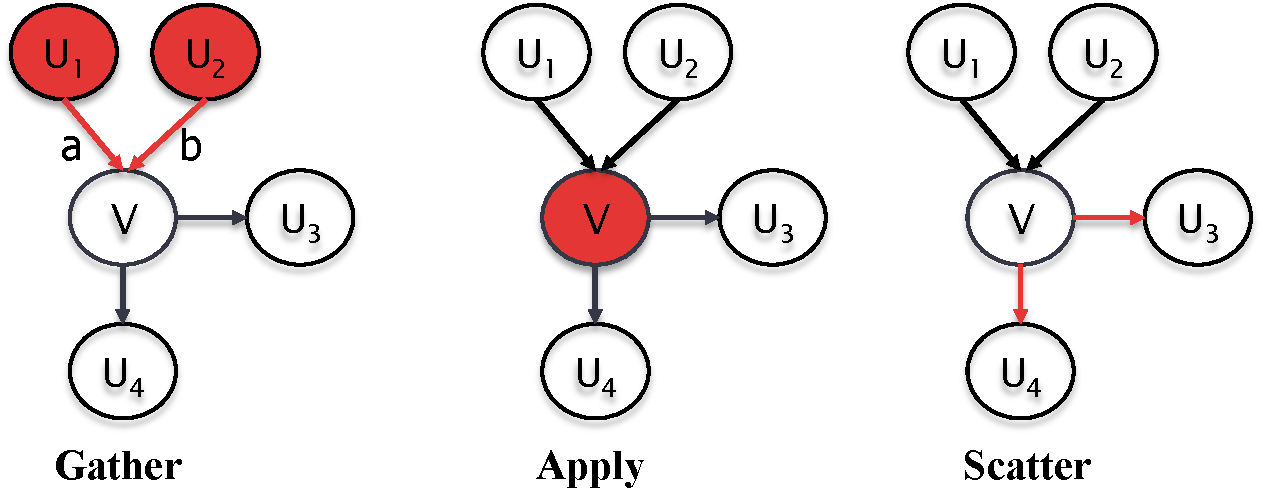
\includegraphics[width=\textwidth]{GAS}
\end{minipage}
\begin{minipage}{0.49\textwidth}
\includegraphics[width=\textwidth]{Strings-design}
\end{minipage}
\caption{\small a) An example of GAS abstraction. b) Three different implementations GPU remoting.}
\label{fig:design}
\end{center}	
\end{figure*}
\end{center}


%\section{System Design Principles}
\label{design1}

\subsection{Multi-tenancy in GPUs}
The frontend/backend model suggests three methods for mapping frontend applications to backend workers (processes or threads), shown in Figure~\ref{fig:design}b.

\textit{Design I.} Each frontend application is mapped to a unique backend process, which then dispatches the actual accelerator (e.g., CUDA) calls to some physical GPUs. This design offers high fault tolerance and security to frontend applications, as it isolates their GPU components in separate backend protection domains (GPU contexts). While used in our  \textit{‘Rain’} scheduler ~\cite{Rain}, as indicated in the figure, a drawback is that a large number of frontend applications will require an equally large number of backend processes, hurting scalability. For NVIDIA GPGPUs, because the CUDA runtime does not allow two different host processes to share the same GPU context, the GPU components of two different applications cannot run concurrently on a single GPU, resulting in GPU context switching overhead and potential GPU core idling.

\textit{Design II.} An alternative design avoids context switching, by packing different application contexts into a single protection domain~\cite{liedtke}, which we term ‘context packing’. Specifically, by mapping each frontend application to a different CUDA Stream, the design creates a single backend thread per device, thus consolidating the GPU components of all frontend applications into a single hosted GPU context. Advantages include (i) minimal backend context switching overheads, reduced further by pinning the per GPU backend threads to certain CPU cores, and (ii) the presence of a single GPU context hosting all frontend applications, which enables the cross-application space-shared use of GPU resources – multi-tenancy. Such efficient GPU space sharing is useful for multi-tenant cloud workloads less concerned with isolation (e.g., Amazon’s web store runs multiple web servers in a single VM, for efficiency in resource usage). It is also useful for pairing applications with different characteristics, e.g., one with high memory bandwidth, the other highly compute intensive, but with their aggregate GPU resource requirements not exceeding those available in the physical GPU. An advantage specific to CUDA is (iii) that by leveraging CUDA streams, all three GPU engines, (a) memory copy from host to device (H2D), (b) from device to host (D2H), and (b) compute, can be concurrently used by different applications, to fully utilize these GPU resources. Potential shortcomings of the design are that (1) it is susceptible to faults, e.g., if the master thread managing all requests to a particular GPU crashes, all frontend applications relying on it are affected, (2) a malicious application can corrupt the entire GPU context or gain unauthorized access to other application’s data, (3) the single master thread has to continuously synchronize with all frontend applications to ensure fair overall progress and pipelined execution, which significantly adds to the complexity and overhead of the runtime, and (4) a blocking call, e.g., cudaDeviceSynchronize(), made by one application will block all other applications sharing the same GPU context, and deferring such call for a long time will lead to application starvation.

\textit{Design III.} \textit{Strings} ~\cite{Strings} adopts a hybrid of Designs I and II, leveraging the fact that for NVIDIA GPUs, from CUDA v4.0 onwards, GPU contexts are hosted per process per device, which implies that the GPU operations invoked from threads within a single host process can run concurrently on a GPU, while those from separate processes are still multiplexed by the device driver. As shown in Figure~\ref{fig:design}b., in Strings, therefore, the GPU components of all frontend applications sharing a particular GPU are mapped to separate backend threads of the same per GPU backend process, with their respective GPU operations invoked via separate CUDA streams. The design has reduced overhead compared to Design I, due to reduced thread vs. process context switch overheads. While not providing complete isolation, the design improves on Design II in that faults can be localized to certain threads. Most importantly, the GPU operations from different applications can run concurrently, thereby inheriting all of the benefits of space and time sharing of Design II. Further, as GPU requests are channelized through separate backend threads, overheads of request synchronization and of pipelined execution are reduced to a minimum, and properties like fair progress for GPU applications are much easier to implement.

\begin{figure}[h]
\begin{center}
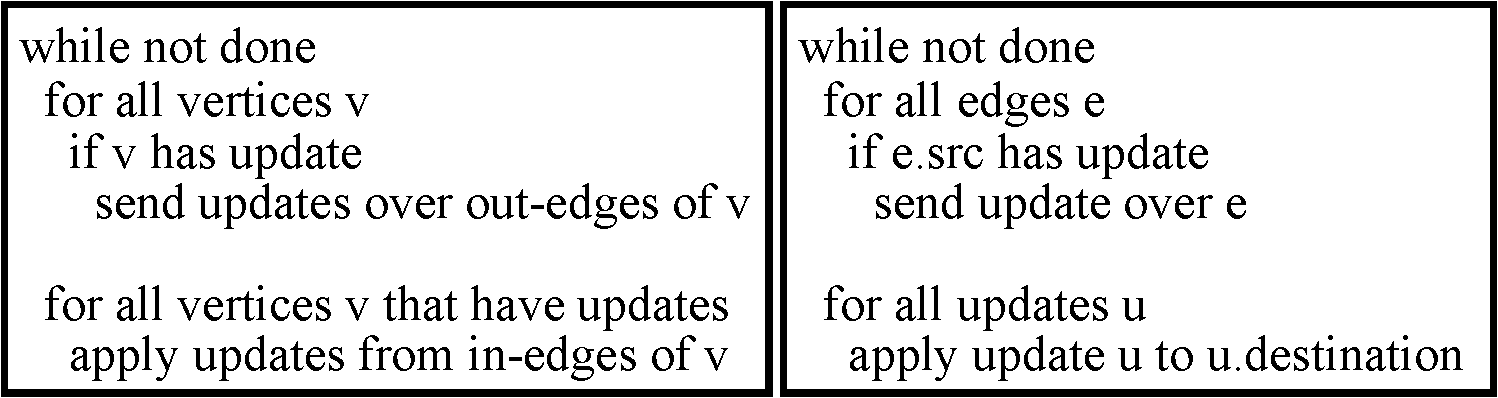
\includegraphics[width=0.75\textwidth]{hybrid-model}
\caption{\small Vertex-centric and Edge-centric Scatter-Gather.}
\label{fig:vertex-edge}
\end{center}
\end{figure}


\subsection{Out-of-Core Graph Processing on GPUs}
\textbf{Hybird Programming Model.}
Figure \ref{fig:vertex-edge} shows two common ways to implement graph algorithms with GAS: edge- vs.vertex-centric execution, which differ in whether the
Scatter and Gather phases iterate over and update edges vs.vertices. GraphLab~\cite{graphlab}, Pregel~\cite{pregel} and GraphChi~\cite{chi} use the vertex-centric model, while X-Stream~\cite{xstream} uses the edge-centric model. In comparison, a more efficient implementation will be to employ a hybrid programming model using both edge- and vertex-centric operations. This is because in the GAS model, different processing phases have different types of parallelism and consequently, offer different parallelism opportunities, coupled with different memory access characteristics. For instance, an edge-centric model should be used in the Gather Phase, because a GPU hardware thread will then be assigned to work on behalf of an edge in the graph. This is preferable to the vertex-centric model, because first, real-world graphs commonly have more edges than vertices, thus giving rise to higher degrees of parallelism and decreased GPU core idling. Second, in the vertex-centric approach, each vertex receives information from multiple in-edges, resulting in a consequent need for synchronization or atomics to order the receive operations from each of the in-edges. This could potentially degrade the overall performance. The same observations hold for using the edge-centric model in the Scatter Phase. In contrast, in the Apply Phase, there are parallelism opportunities only over the vertex set, thus favoring a vertex-centric model.

\label{fig:prob}
\begin{center}
\begin{figure*}[t]
\begin{center}
\begin{minipage}{0.49\textwidth}
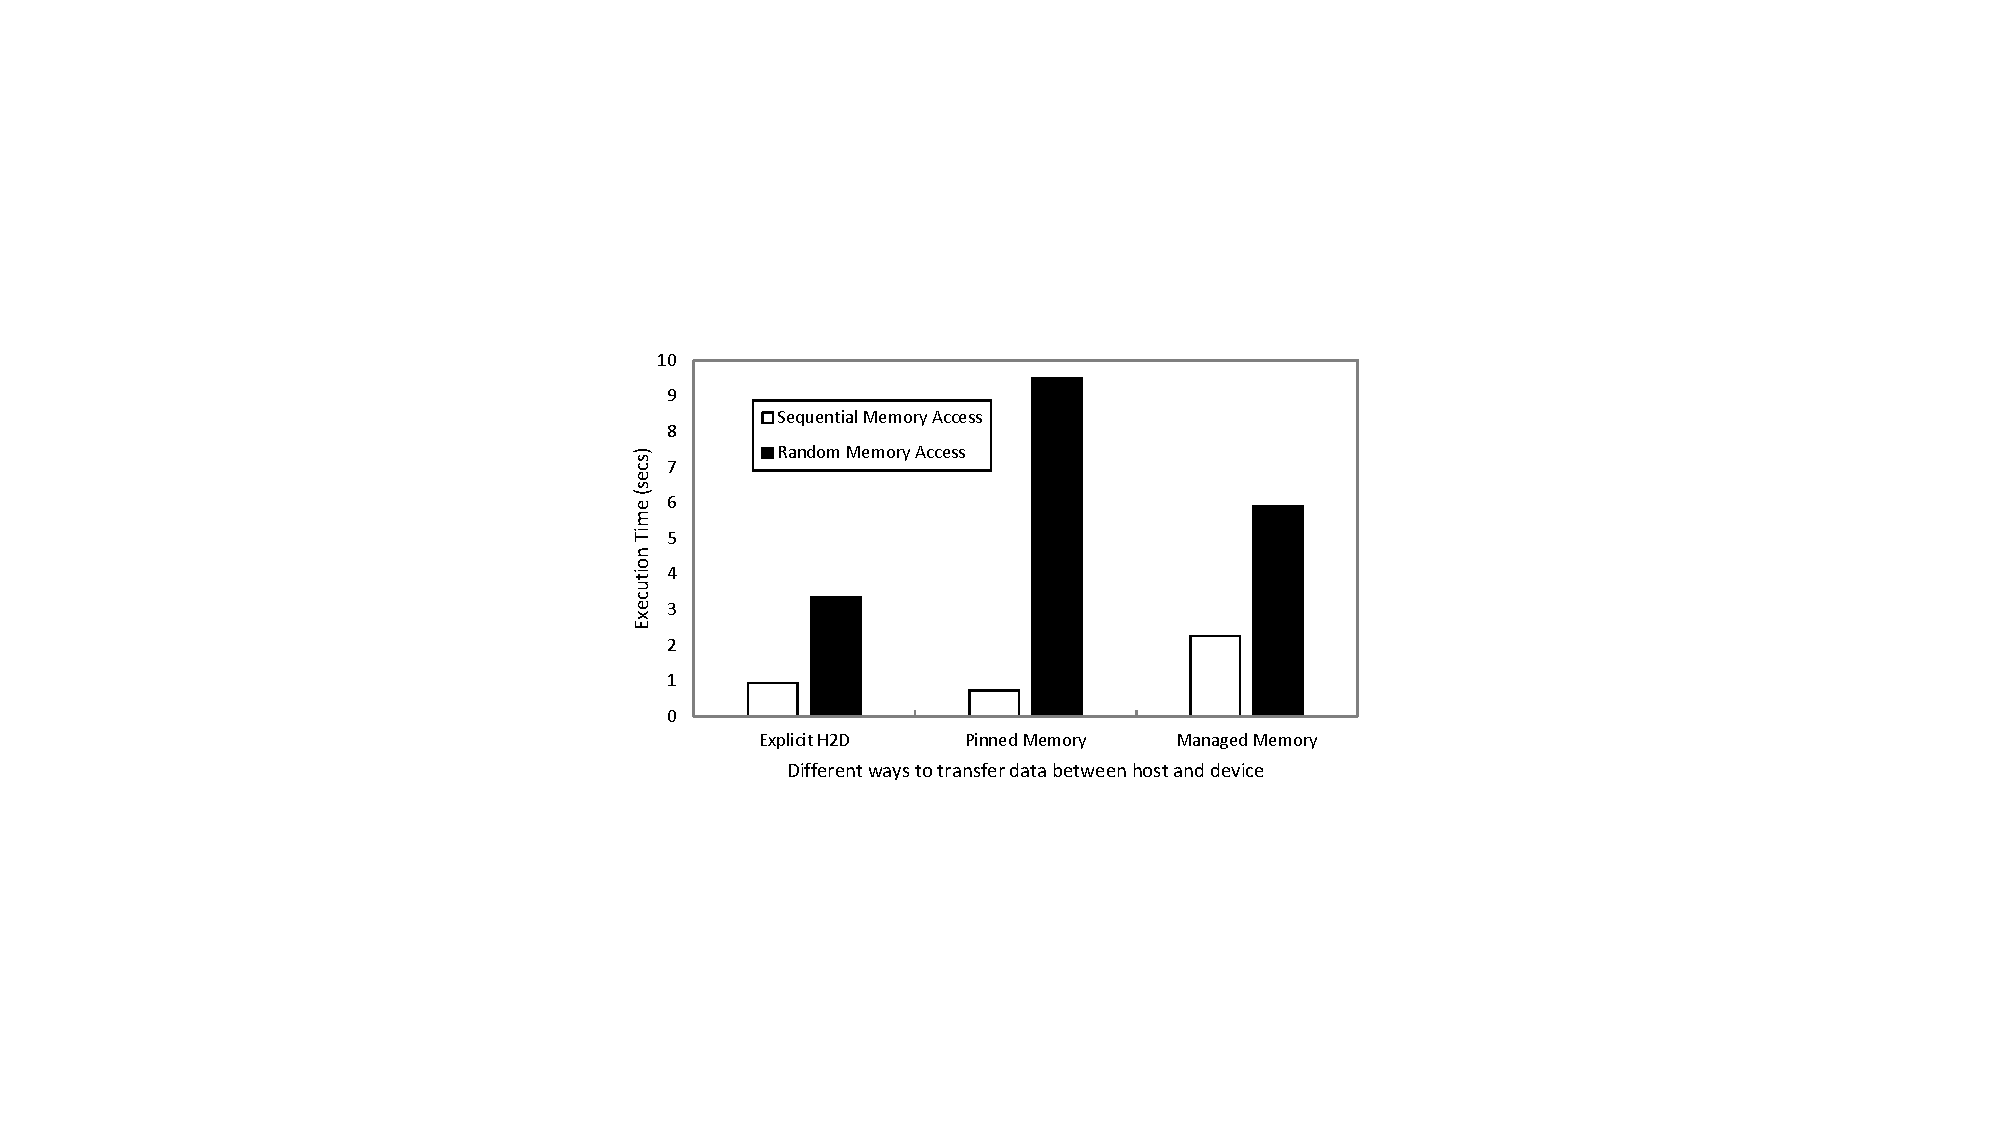
\includegraphics[width=\textwidth, height=4.5cm]{transfer}
\end{minipage}
\begin{minipage}{0.49\textwidth}
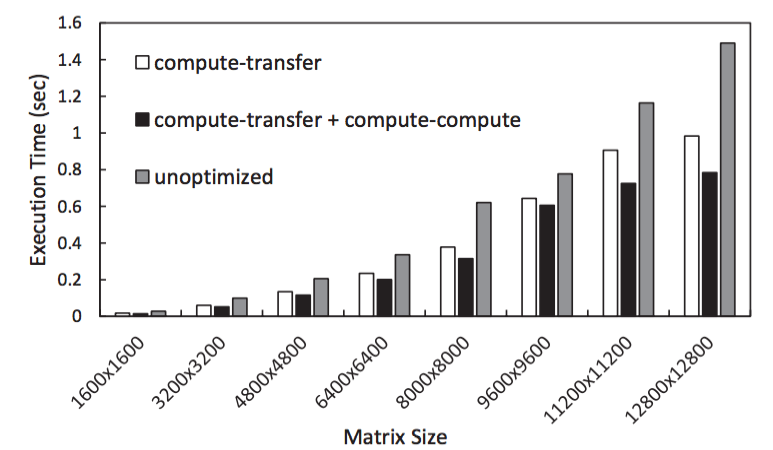
\includegraphics[width=\textwidth, height=5.5cm]{Matrix}
\end{minipage}
\caption{\small a)Performance of transferring 100,000,000 double elements, using three techniques for data exchange between CPU and GPU. b) Performance benefits of using a combination of compute-transfer and compute-compute schemes for processing matrix multiplication with different input sizes. Stripe size=50, which refers to the contiguous number of rows of the matrix being fetched into the GPU memory as a chunk.}
\label{fig:transfer}
\end{center}	
\end{figure*}
\end{center}

\textbf{Characterization of Buffers in Play. }
Graph data chunked to fit into GPU memory and to be moved from host to GPU, is comprised of edges that have either a destination or a source vertex in some well-defined graph partition. Henceforth termed shards, such chunks reside in memory buffers that experience different access patterns. We characterize such access patterns in order to appropriately map corresponding memory buffers to the memory abstractions exposed by current GPUs. In terms of data movement, buffers can be classified as static vs. streaming buffers. Static buffers are copied only once to GPU memory, typically in the Initialization phase. They remain there for the lifetime of the graph execution. An example is a vertex set of a graph that fits into GPU memory. Streaming buffers, on the other hand, are moved in and out of GPU memory as processing progresses, and at any point in time, a particular instance of some streaming buffer resides in GPU memory, e.g., a subset of a graph’s edge set. In the GAS programming model, static buffers are accessed in all three phases, while streaming buffers only appear in a single phase. Another way to characterize buffers is by their access rules, such as read-only or read/write access. For example, vertex and edge data buffers (containing mutable states) have both read and write access patterns, while the vertex set (containing immutable vertex IDs) is read-only. Based on these attributes, the GR runtime makes decisions on whether or not to transfer certain buffers back to the host . Finally, buffers can be classified in terms of the spatial locality of their accesses, e.g., random or sequential access. For example, in the edge-centric approach, there are random accesses to the vertex set.
Once characterized, buffers are mapped to the different memory abstractions exposed by GPU, which at minimum, contain slow and fast memory (e.g., host memory and GPU memory). In the different phases of the GAS model, there are a mix of random and sequential accesses to the input buffers (e.g., edge/vertex sets). For this mix, we posit that random access to slow memory is much more expensive than random access to faster memory, whereas for sequential access, memory-level parallelism and prefetching can help mask slower memory access speed. Therefore, due to the limited fast memory size (GPU), we choose to map all sequential accesses in a GAS phase to the slower CPU memory and all the random accesses to the faster GPU memory. We next validate these assumptions. Figure~\ref{fig:transfer}a. depicts the performance of three techniques for data exchange between host and GPU (through CUDA runtime APIs): (a) explicit data transfer using cudaMemcpy() or Explicit H2D; (b) Pinned Memory using Unified Virtual Addressing (UVA), in which data is transferred implicitly by the CUDA runtime but the memory is allocated as locked memory on the host side; and (c) Managed Memory (introduced in CUDA 6 as Unified memory), where data is transferred between host and device on demand. The measurements shown in the figure illustrate that in the case of sequential memory access, Pinned Memory performs the best, because the accesses directly translate to memory loads/stores operations over the PCIe in which (i) sequential accesses benefit from memory level parallelism (MLP) and (ii) software-level prefetching can hide communication overheads. In the case of random access, Explicit H2D performs the best and Pinned Memory performs the worst. In other words, random access performs best when data resides in faster GPU memory, and the performance of the Pinned Memory degrades as the load/store memory operations over the PCIe fail to benefit from prefetching (after all, accesses are random!). Since Pinned Memory performs the best for sequential accesses, one straightforward approach is to or- ganize graphs such that all memory accesses are sequential. However, because of the significant number of random accesses to either the edges or vertices of a graph in at least one phase of the GAS model, this is not a viable solution for GR as the benefits of sequential accesses are overshadowed by the huge overhead of the random accesses to the slow memory. In response, GR uses explicit data transfer as the mechanism for transferring data between host and device, in way that aim to leverage GPU memory coalescing and software prefetching for the sequential accesses.Although certain performance benefits may exist through intellegent runtime buffer-type selecting. 

\textbf{Coordinated Movement Computation and Data.}
The spatial choice of where in memory to locate data requires an associated temporal choice in when to perform data movement between host and GPU memories. GR uses two methods to attain high performance: (1) hide communication costs by overlapping GPU computation with necessary data transfers, and (2) utilize the GPU’s inherent high degree of potential internal parallelism. (1) is obtained via software-based prefetching to move shards into GPU memory while GPU kernel(s) are being executed. (2) is realized by leveraging underutilized GPU resources (idle threads) caused by the irregular nature of graph processing. It involves (i) detecting such idle threads, using the computation frontier information available to the GR runtime, and (ii) initiating the execution of new shards when idleness is present (note that shards within a single GAS phase do not have data dependencies, so they can be processed in parallel). GR accomplishes this by automatically launching multiple kernels (within the same context), according to the resources available in each GAS phase. Denoting (1) as compute-transfer scheme and (2) as a compute-compute scheme, Figure~\ref{fig:transfer}b. shows the performance benefits obtained from using these approaches vs. an unoptimized scenario when processing a large matrix that doesn’t fit into GPU memory, thus clearly demonstrating the importance of coordinating computation with data movement. We will use these two schemes for processing graph algorithms across phases in the GAS model.

\subsection{Evolving Graph Analytics on GPUs}
There are two major scenarios in terms of analysis of evolving graphs: 1) Offline evolving graph processing where multiple versions of the graph are stored and analyzed to observe the change in certain graph properties over time. 2) Online evolving graph processing that involve real-time continuous query processing over streaming updates on the evolving graph. our solution focuses on online graph analytics. For the rest of the document, evolving graph processing implies online graph analytics.
There are broadly three key characteristics of evolving graphs that dictate the design decisions for our framework:
\begin{itemize}
\item Computation overlap in a sequence of evolving graph versions
\item Data or working set overlap in a sequence of evolving graph versions
\item Static vs dynamic execution runtime
\end{itemize}

{\bf Computation overlap and programming model.}
Between multiple versions or snapshots of an evolving graph the vertex states or values for many vertices remain the same over time and therefore their recomputation is essentially redundant. We define an inconsistent vertex to be a vertex for which one or more properties are affected when the update batch is applied. For example, while calculating out-degree of vertices, an addition or deletion of edge $(v\textsubscript{i},v\textsubscript{j})$ only makes vertex vi inconsistent. For BFS however, addition of edge $(v\textsubscript{i},v\textsubscript{j})$ makes $v\textsubscript{j}$ and all vertices that are “downstream” from $v\textsubscript{j}$ inconsistent. One can consider the entire vertex V to be inconsistent by default. In many scenarios, changes affect only a very small subset of the graph (e.g. calculating out-degree) and computing the vertex states only for those inconsistent vertices and feeding the vertex states from the previous graph versions for the rest of the vertices will significantly reduce the computation time. This observation is the key motivation of the proposing a new programming model for incremental graph processing. To reduce overheads, we aim to build a set of inconsistent vertex sets and sub-graphs that are affected by an update batch and then reduce the incremental graph problem to a sub-problem in the GAS model.

\textbf{Working set overlap and data structure choice.}
When choosing the data structure to store the evolving graph with n vertices and m edges we have multiple options. Adjacency matrices allow for fast update with both insertions and deletions taking O(1) time but require a lot of space O($n\textsuperscript{2}$). Adjacency lists are space efficient O(m+n) and allow fast updates but graph traversals are very inefficient due to non-contiguous memory nodes in the adjacency edge list. Compressed Sparse Row (CSR) formats provide both space efficiency combined with fast traversal (often can be easily parallelized) by storing offsets rather than all the valid fields in the adjacency matrix. But inserts and deletes are very expensive because each update requires shifting of the graph data throughout the compressed array to match the compressed format.
Another key observation to make here is that there is huge overlap in the edge and vertex set between consecutive versions of an evolving graph. Formally, if the graph evolved from G to G’ in certain time epoch t and let $\delta\textsubscript{1} = G' - G$ (insertions), $\delta\textsubscript{2} = G - G'$(deletions) then $G \cap G' = G - \delta\textsubscript{2}   = G' - \delta\textsubscript{1}$ is the overlap between the working set of the two consecutive versions.
In order to allow faster updates to the graph and run both the incremental and static graph algorithms more efficiently, GraphIn uses a hybrid data structure involving edge-lists to store incremental updates and compressed format to store the previous static version of the graph. As mentioned above, the edge-list allows for faster updates, and it does this without adversely affecting the performance of incremental computation. The compressed matrix format allows for faster parallel computation over the entire static version of the graph.  The framework merges the update list and the static graph whenever required.

\textbf{Static vs dynamic runtime.}
Runtime of online graph analytics varies widely depending on the algorithm and the update list. There are scenarios when the incremental algorithm affects only a small or local portion of the graph (e.g., makes a small subset of the graph inconsistent) and changes to the graph require accesses proportional to the size of the update batch. Per-vertex properties that depend on  a fixed radius affect only a local portion of the graph and hence the runtime is proportional to the update batch size (e.g., for triangle counting and in-degree calculation). On the other hand there are classes of incremental algorithms where the graph property depends on paths and can cause a large portion of the graph to become inconsistent, resulting in a complete  recomputation of the graph. In this scenario, incremental processing won’t achieve any performance benefit over  static recomputation and might even result in a performance degradation due to the overheads associated with incremental execution. To handle both the scenarios efficiently,  we need heuristics to select either the incremental or static execution pathway. The decision is made dynamically and taken based on a set of built-in or user-defined graph property checks (e.g., vertex degree information) and the fraction of inconsistent vertices in the update batch that meet the criteria. More precisely, if the update is predicted to require access to and/or affect a small portion of the graph then the incremental execution path is taken, otherwise the update is merged with the static graph and the entire graph is recomputed.  Going back to the BFS example, if 90\% of the inconsistent vertices in an update batch are of high degree, a large portion of the graph is likely to be impacted, so the static execution path is taken. The metadata that is used to decide between static and incremental graph execution is discussed in detail in the architecture section.



%\section{Applications}
\label{applications}

\subsection{GPU Cloud Workload}
To evaluate multi-tenancy in GPUs, applications from the CUDA SDK and the Rodinia benchmark suite are chosen to create a pairwise workload mix of short (\textless  10sec) and relatively long (10-55 sec) running jobs. We assume typical cloud services to operate in response to end user requests, with each individual service running for some small amount of time to complete a single request, but with the requirement of being highly responsive. This assumption matches the service behavior reported by Amazon, for instance, for its web service infrastructure. However, the actual types of service instances being used will vary, which we reflect by carefully choosing for the evaluation a diverse set of application kernels, like image processing (e.g., matrixmult), financial (e.g., BlackScholes), etc. The outcome is a workload mix with many short running rather than a few long running sets of jobs.

\subsection{Graph Algorithms} We will be evaluating our graph processing framework on GPUs using popular algorithms, including Breadth First search (BFS), Page Rank (PR), Single-Source Shortest Paths (SSSP), and Connected Components (CC). Algorithms requiring undirected graphs as inputs, e.g., connected components, are stored as pairs of directed edges.
Some incremental graph algorithms must accommodate inserts and deletes from the latest update batch in each iteration of the algorithm. These updates must be applied to the original graph G before the next update batch is considered. In general, this is the case for graph algorithms that calculate global properties, like BFS, which needs to consider any added or removed edges before recalculating vertex depths. Other algorithms, often ones that compute over properties that are semi-localized within a graph, need to only accommodate per-batch deletes e.g. connected components algorithm. Finally, there are algorithms where each incremental iteration has no dependency on inserts or deletes from the previous batch. This is often the case for algorithms that only utilize local properties. Examples include the computation of clustering coefficients, triangle counting, calculating vertex degree etc. In such cases, both inserts and deletes may be deferred. 

Based on these observations, we support three merge patterns:
\begin{itemize}
\item \textbf{All-Merge:} Both inserts and deletes are merged with G at the end of the incremental GAS loop.		
\item \textbf{Partial-Merge:} Either deletes or inserts are merged with G at the end of the incremental GAS loop. The framework defers applying the rest of the updates to the original graphs.
\item \textbf{No-Merge:} Neither inserts nor deletes from the update batch are merged with G at the end of the  incremental GAS loop. The framework defers applying both inserts and deletes. 
\end{itemize}

We will be evaluating our incremental graph processing framework using applications from the above three classes of algorithms, including Clustering Coefficient (CCof), Connected Components (CC) and Breadth First Search  (BFS). These algorithms are classified as no-merge (CCof), partial-merge (CC) and all-merge (BFS) as described in the above. 

 
%\section{Evaluation}
\subsection{Graph Datasets}
We will evaluate the performance and efficiency of our framework using a mix of real- world and synthetic datasets. Examples of few real-world datasets include Facebook interaction graph and graphs from the University of Florida Sparse Matrix collection e.g. LiveJournal. The synthetic datasets are obtained from the Graph500 RMAT data generator using scales ranging from 20 to 23 graphs with average degree of 16 per vertex.

\subsection{Evaluation Platform}
Evaluations will be on a typical heterogeneous HPC node equipped with 16-core Intel Xeon E5-2670 processors running at 2.6 GHz with 32 GB of DDR3 RAM, and one attached NVIDIA Tesla K20c GPU with 13 SMX multiprocessors and 4.8 GB GDDR5 RAM. All the runs will be compiled with the highest optimization level flag.

\label{evaluation}



\chapter{Strings: Multi-tenancy in Accelerator-based Servers}

%\section{Introduction}
Cloud and server infrastructures routinely use GPUs to service computationally intensive client workloads, for online gaming~\cite{nvidia-game}, multimedia services~\cite{element} and image processing~\cite{adobe}, financial codes~\cite{zillians}, data mining~\cite{GPUmine} and search~\cite{GPUsearch}, and to support the needs of next generation applications like perceptual computing~\cite{GPU29, GPU30, GPU31, GPU32, GPU33}. This trend is mirrored by GPU offerings by cloud providers like Amazon ECC~\cite{amazon}, Nimbix~\cite{nimbix}, Peer1 Hosting~\cite{peer1}, and Penguin Computing~\cite{penguin}. 

The effective use of GPUs in these multi-tenant server and cloud infrastructures, however, challenges the current model of static GPU provisioning, in which applications explicitly and programmatically select the GPU devices on which they wish to run. Such static GPU assignments will inhibit concurrency, particularly with the varying workloads imposed by web applications. For instance, during peak demands for certain services, their GPU devices will be heavily utilized while other services' GPUs will be idle or underutilized. Additional GPU underutilization will be caused by application-specific variations in their fraction of CPU vs. GPU execution time, for reasons that include an inability to parallelize certain application components and/or limited GPU residency vs. the costs of host-GPU data transfers.

The \textit{Strings} scheduler described in this chapter adopts a multi-tenant model in which accelerators like GPUs are treated as first class schedulable entities~\cite{gdev, gvim, ravi, pegasus}, by overriding the device selection calls made by applications and then managing their GPU calls with a two-level scheduler: at the higher level, on each platform, balancing workloads across the multiple GPUs attached, and at the GPU device level, reducing core idling via multi-tenancy and the judicious overlap of GPU execution with host-GPU data movements. Additional performance improvements are derived from dynamically merging the GPU contexts of different applications and by providing dynamic feedback about fine-grain application characteristics from device-level schedulers to the workload balancer.

Using \textit{Strings} with workloads drawn from diverse classes of cloud applications, this chapter presents and evaluates GPU scheduling policies distinct from prior work in their explicit consideration of data movement to/from the GPU device. (1) The Phase Selection (PS) policy co-schedules on the same GPU those applications that currently operate in different phases – computation vs. communication -- of their combined CPU/GPU execution. Using PS results in an average speedup of \textbf{6.41x} over static provisioning with the CUDA runtime. (2) Advanced feedback-based policies, termed Data Transfer Feedback (DTF) and Memory Bandwidth Feedback (MBF), capitalize on the advantages offered by CUDA streams and by Strings’ built-in support for merging GPU contexts belonging to different applications. DTF collocates applications with contrasting data transfer times to maximize the concurrent use of a GPU's memcpy vs. compute engines. MBF improves overall performance by concurrently executing and hiding the large memory latencies seen by a memory bound application by switching to a compute bound application. DTF and MBF achieve notable improvements in average system throughput, by \textbf{8.06x} and \textbf{8.70x}, respectively, compared to the commonly used CUDA runtime. (3) Further improvements in performance are derived from dynamic changes to the workload balancing policies being used in response to device-level observations of altered behavior in the GPU tasks being run.


This chapter makes following technical contributions:
\begin{itemize}
\item A two-level hierarchical scheduler where workload balancing intelligently binds each application’s GPU component to an appropriate GPU, along with a device- level, per-GPU scheduler that handles GPU resource sharing for the multiple tenants mapped to a single GPU, to improve application performance while also meeting system-level goals like high throughput, fairness, etc.
\item Support for multi-tenancy, termed the Context Packer, which dynamically packs the GPU contexts of multiple applications into a single context, to achieve high GPU utilization and low context switching overhead.
\item Dynamic feedback from device-level schedulers to workload balancer, to inform the global decisions made by the latter about the characteristics of the applications being scheduled by the former.
\item A novel GPU scheduling policy, called Phase selection (PS), which maximizes the concurrent use of a GPU’s memcpy vs. compute engines, by smartly selecting applications currently running in different phases of their combined CPU/GPU execution.
\item Advanced feedback-based policies like DTF and MBF that exploits the advantages offered by CUDA streams by collocating applications with contrasting behavior, in terms of data transfer and memory intensity, to achieve extreme performance benefits.
\end{itemize}


\section{Background and Motivation}
\subsection{Scheduling Crisis in GPU Multitenancy}
Current programming models continue to treat GPUs as devices chosen by applications. There are several issues with the consequent programmer-defined selection of target GPUs. First, applications running on a multi-GPU node may compete for the same GPU, thus not able to leverage availability of multiple on-node GPU accelerators and leading to the serialization of GPU requests that  otherwise  could  have  been served in parallel. We define such conflicts as \textit{static collisions} between applications' GPU requests. Second, since applications are unaware of each other’s GPU usage, e.g., their relative GPU intensities, they cannot assess the performance implications of sharing a single GPU. We define this as a \textit{character collision} between the requests from two or more applications sharing a GPU. Both static and character collisions become even more critical when nodes have heterogeneous GPUs with differing capabilities in terms of their compute, memory capacities, and bandwidths. 
	
	The importance of collisions is underlined by the fact that most cloud applications driven by end user requests vary substantially in their compute and memory characteristics and therefore, have difficulties in fully utilizing both the compute engines and memory capacities of GPUs. We demonstrate this in Figure~\ref{fig:cloud-workload}, with cloud applications deployed using the CloudBench~\cite{cloudbench} infrastructure, for exponentially distributed request arrivals. The color-coding in the figure indicates the levels of compute and memory utilization of the applications, varying from heavily utilized (red $>$ 90\%) to under-utilized (green $<$ 10\%). Some of these applications are compute intensive, such as graph algorithm Breadth First Search (BFS), some are memory intensive – financial algorithm Monte Carlo (MC), and some exhibit average utilization levels, like OPENCV~\cite{opencv} face detection (FD). Note that frequent GPU idle intervals occur even for efficient GPU codes like Monte Carlo.
	
\begin{figure}[t]
\centering
%\includegraphics[width=3.2 in]{figures/cloud-workload.pdf}
\includegraphics[width=0.75\textwidth,height=\textheight,keepaspectratio]{figures/cloud-workload.pdf}
\caption{Compute and memory characteristic of various GPU-based cloud applications. }
\label{fig:cloud-workload}
%\vspace{-1\baselineskip}
\end{figure}

\begin{figure}[t]
\centering
%\includegraphics[width=3.2 in]{figures/cloud-workload.pdf}
\includegraphics[width=0.75\textwidth,height=\textheight,keepaspectratio]{figures/GPU-utilization.pdf}
\caption{GPU utilization of Monte Carlo requests following exponential distribution of request arrival with sequential vs. concurrent execution. }
\label{fig:GPU-utilization}
%\vspace{-1\baselineskip}
\end{figure}

Another issue with current GPU programming models is that although each GPU can internally contain thousands of cores, application uses it as a single SIMD engine~\cite{GPU25}, which means that the multiple GPU contexts created by host threads can share a GPU only over time, but not in space. CUDA 4.0 addresses this problem by allowing multiple threads within a single host process to share the same GPU context, but GPU utilization could be improved further with true GPU multi-tenancy. We demonstrate this opportunity by manually dispatching multiple sets of independent Monte Carlo requests, again following an exponential distribution of inter-arrival times, over different CUDA \textit{Streams}~\cite{cuda7} from the same GPU context. Figure~\ref{fig:GPU-utilization} shows GPU usage peak and idle periods to be much more uniform compared to their sequential execution. This is because keeping a single GPU context avoids context switching overhead and this eliminates unnecessary GPU idling during context switching (the `glitches' in the figure), as in the case of independent sets of web requests driving their execution.

The illustrative examples above motivate key properties of the  Strings  approach  to effective multi-tenancy in GPU-based servers: (1)  load  balancing is needed to avoid static collisions, (2) device-level scheduling must be cognizant of character collisions   and   provide  such feedback  to  the   load  balancer,  (3)   additional   functionality   is  needed  to  achieve resource management goals like fairness, high throughput, etc., and (4) there should be system-level support for reducing GPU core idling when some application's context cannot fully utilize a single GPU. We next describe the Strings infrastructure and its utility for realizing and experimenting with effective scheduling strategies for cloud and multi-tenant workloads using GPUs.

\begin{figure}[!t]
\centering
%\includegraphics[width=3.2 in]{figures/cloud-workload.pdf}
\includegraphics[width=0.85\textwidth,height=\textheight,keepaspectratio]{figures/GPU-remoting.pdf}
\caption{Architecture of GPU Remoting. }
\label{fig:GPU-remoting}
%\vspace{-1\baselineskip}
\end{figure}
\section{System Design Principles}
\subsection{Future GPU Servers and gPool}
Scheduling the potentially multiple GPUs in future server platforms demands (i) the logical aggregation of all GPUs to make them visible to the scheduler and then (ii) decoupling the CPU-GPU associations programmed into GPU-based applications. Strings adopts from previous work (e.g., GVim~\cite{gvim}, vCuda~\cite{vcuda}, rCuda~\cite{rcuda}, Pegasus~\cite{pegasus}, gVirtus~\cite{gvirtus}) an API-driven separation of an application's CPU from its GPU components. As shown in Figure~\ref{fig:GPU-remoting}, (i) a \textit{frontend} implemented as a CUDA runtime interposer library dynamically links with the application, responsible for intercepting the CUDA runtime API calls, and (ii) a \textit{backend} is realized as a daemon responsible for receiving GPU requests from the frontend, dispatching the CUDA runtime library calls to the attached GPUs, and returning error codes and/or output parameters to the frontend. A useful side effect of this architecture is the ability to execute an application's GPU component on a GPU attached to some remote node, termed GPU remoting~\cite{shadowfax}. We do not explore this topic at scale, but use it to create a supernode, which is an emulated high-end multi-GPU server machine   with  more  GPUs  than  those  available  on  today's single physical platforms. For such a supernode, Strings aggregates all GPUs into a single logical pool, termed a \textit{gPool}, for use by the GPU scheduler. The gPool is formed when the GPU virtualization runtime is started and the backend daemons are spawned in each participating node. Each backend collects the information of GPUs in its own node and sends it to the \textit{GPU Affinity Mapper}, discussed later. It assigns a unique GPU id (GID) to each of the GPUs in the pool, builds a mapping from GID to  \verb|<node_id (IP address), local device_id> |pair, called the \textit{gMap}, and broadcasts it to all participating machines.  

With  gPools,  gMap,  and  GPU  request  interposition,  the \textit{Strings} scheduling infrastructure described in this chapter permits any node in the gMap to participate in GPU scheduling. Figure~\ref{fig:GPool} shows the logical transformation of a small number of machines with per-node GPUs into a single supernode with sets of GPUs schedulable via a shared GPU pool. The experimental results in this chapter are obtained with a dual-machine supernode connected via dedicated network links. This purposely small scale setup makes it possible to treat remote GPUs much like NUMA memory is treated in high end servers, ignoring issues like network contention likely to occur for scaleout systems~\cite{shadowfax}.
\begin{figure}[!t]
\centering
%\includegraphics[width=3.2 in]{figures/cloud-workload.pdf}
\includegraphics[width=\textwidth,height=\textheight,keepaspectratio]{figures/GPool.pdf}
\caption{Logical transformatiom of GPU cluster after gPool creation. }
\label{fig:GPool}
%\vspace{-1\baselineskip}
\end{figure}
\begin{figure}[!t]
\centering
%\includegraphics[width=3.2 in]{figures/cloud-workload.pdf}
\includegraphics[width=\textwidth,height=\textheight,keepaspectratio]{figures/Strings-design.pdf}
\caption{Three different implementations GPU remoting.}
\label{fig:Strings-design}
%\vspace{-1\baselineskip}
\end{figure}

\subsection{Design Decisions}
\textbf{\textit{1) Efficient and Robust Scheduling}}

The frontend/backend model suggests three methods for mapping frontend applications to backend workers (processes or threads), shown in Figure~\ref{fig:Strings-design}.

\textbf{Design I.} 
Each frontend application is mapped to a unique backend process, which then dispatches the actual accelerator (e.g., CUDA) calls to some physical GPUs. This design offers high fault tolerance and security to frontend applications, as it isolates their GPU components in separate backend protection domains (GPU contexts). While used in our previous `Rain' scheduler~\cite{Rain}, as indicated in the figure, a drawback is that a large number of frontend applications will require an equally large number of backend processes, hurting scalability. For NVIDIA GPGPUs, because the CUDA runtime does not allow two different host processes to share the same GPU context, the GPU components of two different applications cannot run concurrently on a single GPU, resulting in GPU context switching overhead and potential GPU core idling.

\textbf{Design II.}
 An alternative design avoids context switching, by packing different application contexts into a single protection domain~\cite{liedtke}, which we term `context packing'. Specifically,   by   mapping   each   frontend   application  to  a different CUDA Stream~\cite{GPU5, ravi}, the design creates a single backend thread per device, thus consolidating the GPU components of all frontend applications into a single hosted GPU context. Advantages include (i) minimal backend context switching  overheads,  reduced  further by pinning the per GPU backend threads to certain CPU cores, and (ii) the presence of a single GPU context hosting all frontend applications, which enables the cross-application space-shared use of GPU resources – multi-tenancy. Such efficient GPU space sharing is useful for multi-tenant cloud workloads less concerned with isolation (e.g., Amazon's web store runs multiple web servers in a single VM, for efficiency in resource usage). It is also useful for pairing applications with different characteristics, e.g., one with high memory bandwidth, the other highly compute   intensive,   but  with  their  aggregate  GPU  resource requirements not exceeding those available in the physical GPU. An advantage specific to CUDA is (iii) that by leveraging CUDA streams, all three GPU engines, (a) memory copy from host to device (H2D), (b) from device to host (D2H), and (b) compute, can be concurrently used by different applications, to fully utilize these GPU resources. Potential shortcomings of the design are that (1) it is susceptible to faults, e.g., if the master thread managing all requests to a particular GPU crashes, all frontend applications relying on it are affected, (2) a malicious application can corrupt the entire GPU context or gain unauthorized access to other application’s data, (3) the single master thread has to continuously synchronize with all frontend applications to ensure fair overall progress and pipelined execution, which significantly adds to the complexity and overhead of the runtime, and (4) a blocking call, e.g., cudaDeviceSynchronize(), made by one application will block all other applications sharing the same GPU context, and deferring such call for a long time will lead to application starvation.

\textbf{Design III.} 
Strings adopts a hybrid of Designs I and II, leveraging the fact that for NVIDIA GPUs, from CUDA v4.0 onwards, GPU contexts are hosted per process per device, which implies that the GPU operations invoked from threads within a single host process can run concurrently on a GPU, while those from separate processes are still multiplexed by the device driver. As shown in Figure~\ref{fig:Strings-design}, in Strings, therefore, the GPU components of all frontend applications sharing a particular GPU are mapped to separate backend threads of the same per GPU backend process, with their respective GPU operations invoked via separate CUDA streams. The design has reduced overhead compared to Design I, due to reduced thread vs. process context switch overheads. While not providing complete isolation, the design improves on Design II in that faults can be localized to certain threads. Most importantly, the GPU operations from different applications can run concurrently, thereby inheriting all of the benefits of space and time sharing of Design II. Further, as GPU requests are channelized through separate backend threads, overheads of request synchronization and of pipelined execution are reduced to a minimum, and properties like fair progress for GPU applications are much easier to implement.

\textbf{\textit{2) Asynchronous Operation}}

The presence of an explicit interposer affords additional optimizations. First is the removal of blocking calls, by converting all device synchronization calls to their respective stream synchronization counterparts, e.g., cudaDeviceSynchronize() converted to cudaStreamSynchronize(). This ensures that all the applications sharing a GPU, under the umbrella of a single GPU context, are not stalled when one application explicitly synchronizes with the device.

Second is the runtime conversion of all synchronous memcpy operations into their respective asynchronous versions. With this optimization, (i) subsequent CUDA calls that are not dependent on the memcpy operation can proceed without waiting for memcpy calls to finish, (ii) we hide the overhead introduced by the runtime due to interposition, marshaling, RPC, unmarshalling etc, by allowing execution to proceed and overlap even for calls that are dependent on the memcpy operation. For instance, a cudaLaunch() call that depends on a memcpy typically has to wait for the memcpy to complete, but because it is now asynchronous, the runtime layer overhead for cudaLaunch() can be overlapped with the asynchronous data transfer to the device.

Finally, asynchrony can also be achieved for hidden and synchronous runtime API calls that do not have output parameters, by making interposer-based RPCs non-blocking. This does not violate the correctness in single threaded applications as RPC requests from within an application remain in-order but might affect multi-threaded applications where RPCs from separate threads are not guaranteed to be in-order e.g., when cudaLaunch() from one host thread depends on a memcpy from another and an asynchronous RPC makes the former call to be dispatched before the latter. The problem can be corrected with per-device buffer synchronization logic that maintains the application-intended order of GPU operations across multiple threads within a single application.
\begin{figure}[!t]
\centering
%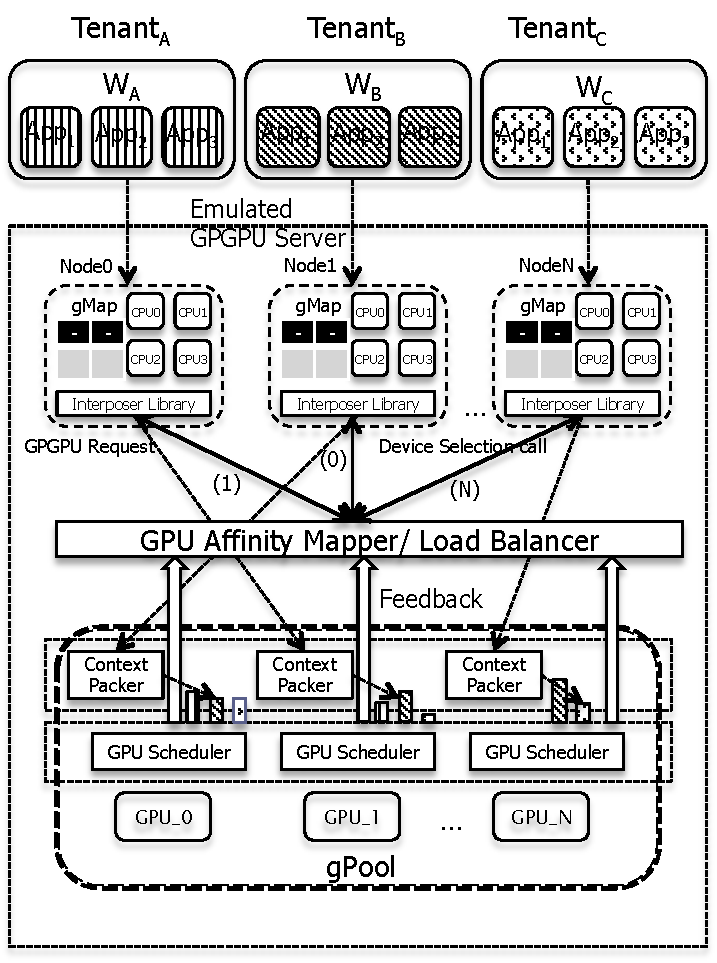
\includegraphics[width=\textwidth,height=\textheight,keepaspectratio]{figures/strings_archi1.pdf}
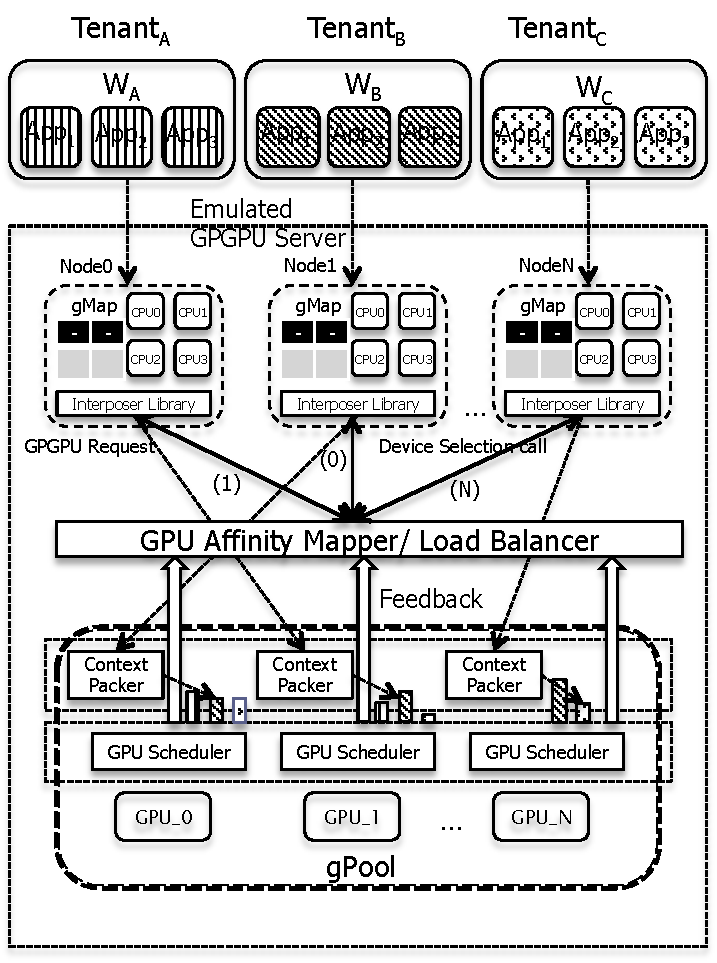
\includegraphics{figures/strings_archi1.pdf}
\caption{Software architecture of Strings.}
\label{fig:strings_archi}
%\vspace{-1\baselineskip}
\end{figure}
\section{Strings Architecture}
We next describe the two-level Strings scheduling infrastructure that avoids static and character collisions of GPU requests, efficiently utilizes the underlying GPU cores with minimum GPU context switching overhead, and meets system goals like throughput and fairness (see Figure~\ref{fig:strings_archi}).

\textbf{GPU Affinity Mapper - Workload Balancing. }To minimize static collisions, the Strings runtime overrides the application's target GPU selection calls, replacing them with decisions made by the GPU affinity mapper/workload balancer. The lifetime of the Strings target device selection call is as follows: (i) an application's cudaSetDevice() call is intercepted by the interposer and forwarded to the workload balancer; (ii) its GPU selection based on static (device capabilities) and dynamic (GPU load, application type, feedback from lower scheduling layer) parameters is returned as a global GPU id (GID) to the interposer; (iii) the interposer uses the GID to acquire a node id and local GPU id from the gMap, and (iv) using GPU remoting, it then forwards the call to some appropriate backend process to bind with the target GPU; (v) the binding is removed when the application exits or calls cudaThreadExit(). The \textit{GPU Affinity Mapper} is also responsible for the cluster-wide aggregation of GPUs through gPool creation. Shown in Figure~\ref{fig:affinity}, it has the following components:
\begin{figure}[!t]
\centering
%\includegraphics[width=3.2 in]{figures/cloud-workload.pdf}
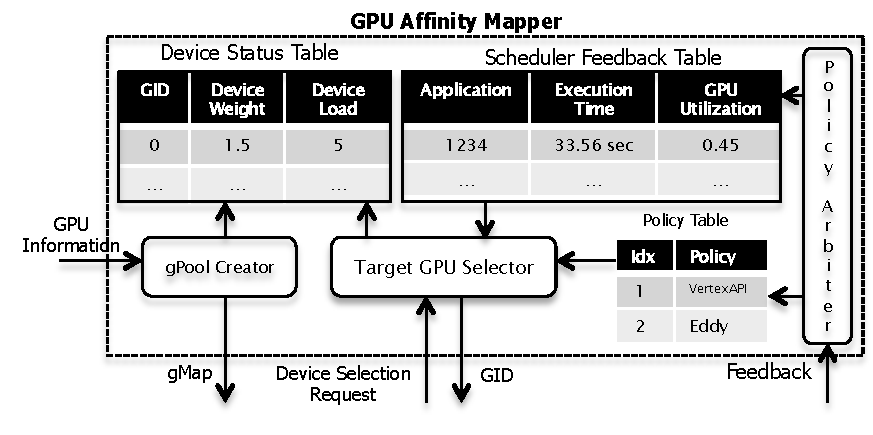
\includegraphics[width=\textwidth,height=\textheight,keepaspectratio]{figures/strings_archi2.pdf}
\caption{The structure of the GPU Affinity Mapper.}
\label{fig:affinity}
%\vspace{-1\baselineskip}
\end{figure}
\begin{itemize}
\item \textbf{\textit{gPool Creator (GC): }}during system initialization, the GC collects device information from the backend daemons of each  node  in  the cluster, assigns a GID to every GPU, creates the gMap and broadcasts it to every node. GC is also responsible for the one time assignment of relative weights to all GPUs based on the device property information received and updating a global data structure, Device Status Table (DST), with this static information. DST also maintains the dynamic states (e.g. current device load) of all the GPUs in the system, which is updated by TGS (explained later) as GPU requests arrive. 
\item \textbf{\textit{Policy Arbiter (PA): }}using the feedback mechanism, the PA receives information about application characteristics like execution time, GPU utilization, data transfer time etc. from the Feedback Engine (FE) of the device-level GPU schedulers and updates a history-based table, Scheduler Feedback Table (SFT), that stores such fine-grain device specific application characteristic information. The PA also triggers dynamic policy switching, upon receiving sufficient feedback information from low-level GPU schedulers.
\item \textbf{\textit{Target GPU Selector (TGS): }}as the core of the workload balancer, it selects an appropriate GPU for an application. Based on the information in the DST and SFT, for each GPU selection request, it computes the target GID using the selected scheduling policy from the Policy Table (PT) and then returns it to interposer, which then maps the application to a particular GPU in gPool. The PT contains two classes of policies, one that uses only the DST, e.g., GRR, GMin, etc., and the other that uses both the DST and low-level feedback information from SFT, e.g., GUF, DTF, etc.
\end{itemize}
\begin{figure}[!t]
\centering
%\includegraphics[width=3.2 in]{figures/cloud-workload.pdf}
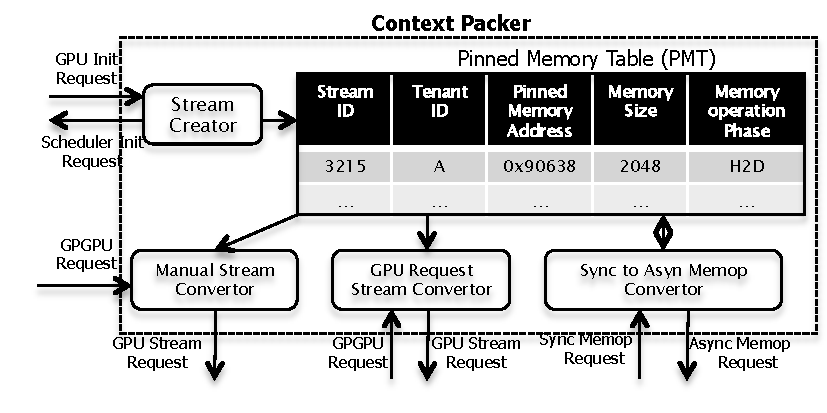
\includegraphics[width=\textwidth,height=\textheight,keepaspectratio]{figures/strings_archi3.pdf}
\caption{The structure of the Context Packer.}
\label{fig:packer}
%\vspace{-1\baselineskip}
\end{figure}
\textbf{Context Packer. } Operating after workload load balancing has assigned a GPU and before device-level GPU scheduling, the Context Packer (see Figure~\ref{fig:packer}), is responsible for packing multiple applications' GPU components that share a GPU, on the fly, into a single GPU context. It also manages the host side locked memory, the dynamic translation of synchronous memory copies to their asynchronous versions, and the dynamic translation of device synchronization calls to their stream counterparts.
\begin{itemize}
\item \textbf{\textit{Stream Creator (SC): }}when the first GPU request from an application arrives, SC creates a separate CUDA stream object for it, calling cudaStreamCreate(), the handler to which is stored in a thread local storage. Using this handler, subsequent requests from the application are dispatched over the stream. On cudaThreadExit() or application exit, SC tears down the stream by calling cudaStreamDestroy() on the stream handler.
\item \textbf{\textit{Auto Stream Translator (AST): }}dynamically translates all GPU operations from an application targeted over the default  stream  (stream 0)  to use the stream created by the SC. E.g., cudaConfigureCall(),   when  called  without  an  explicit stream handler in its call parameters, is targeted onto stream 0, and  AST uses the stream handler for this particular application to translate the call to use that stream.
\item \textbf{\textit{Sync Stream Translator (SST): }}the GPU calls that synchronize the application and the device are converted to their CUDA stream counterparts by the SST, e.g., cudaDeviceSynchronize()    is     converted    to     cudaStreamSynchronize(). This ensures that all of the applications packed into a GPU context associated with a particular GPU are not blocked when one of them explicitly tries to synchronize its host thread with the device. 
\item \textbf{\textit{Memory Operation Translator (MOT): }}translates all memory copies to their asynchronous versions using a per device data structure called Pinned Memory Table (PMT).  PMT stores the active host and device pointers associated with all such memory copy calls and is also responsible for keeping track of the current memory copy phase (e.g., H2D) of an application, storing the stream handler, the application id, tenant id, etc. MOT allocates host locked memory of the size of the host buffer for every such memory copy operation, copies the content of the host buffer into it, and stores both the host and device pointers in the PMT. It then creates an asynchronous version of the memory copy call (e.g. cudaMemcpyAsync()) using the host pointer. On the application’s next device synchronization call or a device to host memory copy, the MOT searches for the device pointer in the PMT and frees the corresponding host memory. When the application invokes the cudaThreadExit() or exits, the MOT frees all outstanding active host pointers in the PMT associated with the application.
\end{itemize}
\begin{figure}[!t]
\centering
%\includegraphics[width=3.2 in]{figures/cloud-workload.pdf}
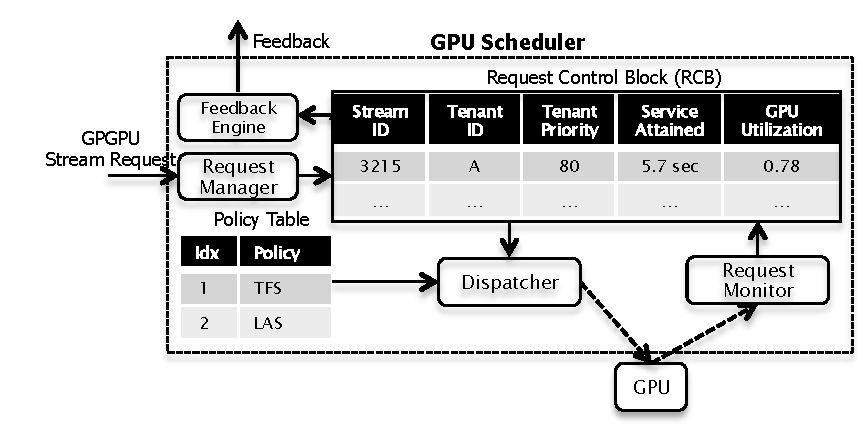
\includegraphics[width=\textwidth,height=\textheight,keepaspectratio]{figures/strings_archi4.pdf}
\caption{The structure of the GPU Scheduler.}
\label{fig:sched}
%\vspace{-1\baselineskip}
\end{figure}
\textbf{GPU Scheduler. }As shown in Figure~\ref{fig:sched}, this per device software layer addresses inter-application interference arising due to the co-location of multiple applications' GPU components on a single GPU. It prioritizes and dispatches GPU requests to physical GPUs in order to meet resource management goals like system throughput, fairness, etc. It is also responsible for monitoring applications bound to the device and sending feedback about their characteristics to the workload balancer.
\begin{itemize}
\item \textbf{\textit{Request Manager (RM): }} registers and unregisters application requests with the GPU scheduler. After the GPU affinity mapper selects the target GPU for an application, the interposer library makes a cudaSetDevice() call to the selected GPU using the GPU remoting infrastructure. On receiving the request, the RM registers the application by creating an entry in a per device data structure called Request Control Block (RCB) with stream id, tenant id and application priority, to be used by the GPU scheduler. RCB also maintains application runtime characteristic information, dynamically computed by the Request Monitor discussed later. When the interposer forwards a cudaThreadExit() call, the RM unregisters the application by removing its corresponding entry from the RCB.
\item \textbf{\textit{Dispatcher: }}prioritizes and dispatches GPGPU requests to the device. It uses the application characteristic information from the RCB and makes scheduling decisions based on the selected policy from the Policy Table (PT). In Strings three policies are implemented to achieve system fairness (TFS), high system throughput (LAS), and a combination of fairness and system throughput (PS).
\item \textbf{\textit{Request Monitor (RMO): }}computes GPGPU application characteristics and GPU resource usage. Both the workload balancer and GPU scheduler make use of this monitoring information in their scheduling decisions. We currently monitor the total execution time, total GPU time, data transfer time, memory bandwidth, application phase and kernel configuration information of an application. The RMO updates RCB in some regular time interval.
\item \textbf{\textit{Feedback Engine (FE): }}communicates the application characteristic and local GPU state information, collected by the RMO, to the GPU Affinity Mapper. It retrieves this information from the RCB and feeds it to the SFT when the application request completes. Therefore, when a cudaThreadExit() call arrives, FE piggybacks the feedback information along with the return value of the CUDA call and sends it back to the interposer, which then forwards the same to the GPU Affinity Mapper.
\end{itemize}

\section{Scheduling Policies}
Strings  implements  a  rich  set  of  scheduling  policies,  to achieve two cloud- and server-centric goals: fairness for multiple tenants, coupled with high overall system throughput.
\subsection{Workload Balancing Policies }
Three workload balancing policies across multiple accelerators are suitable for server systems, driven by external workloads like those seen for cloud and web applications.
\begin{itemize}
\item \textbf{\textit{Global Round Robin (GRR): }}assigns incoming applications to the GPUs in the gPool in a round robin fashion.
\item \textbf{\textit{GMin: }} taking into account the differences in application runtimes, GMin enhances GRR by maintaining a record of the number of applications currently bound to a particular device in the \textit{device load} field. GMin chooses the GPU with minimum device load. Because remote GPUs are more expensive to access, GMin breaks ties by giving preference to local GPUs over remote ones.
\item \textbf{\textit{Weighted-GMin: }}considering heterogeneity across GPUs, in terms of compute, memory capacity and bandwidth, the weighted-GMin (GWtMin) policy extends GMin by assigning relative weights to different GPUs and computing weighted minimum load to select a target GPU.
\end{itemize}
\begin{figure}[!t]
\centering
%\includegraphics[width=3.2 in]{figures/cloud-workload.pdf}
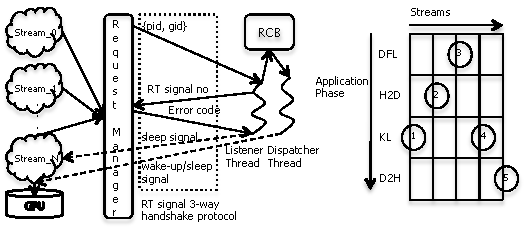
\includegraphics[width=\textwidth,height=\textheight,keepaspectratio]{figures/RT_sched.pdf}
\caption{(a) Real-Time Signal based GPU Scheduler (b) Phase Selection Scheduling Policy. }
\label{fig:RT_sched}
%\vspace{-1\baselineskip}
\end{figure}
\subsection{GPU Scheduling Policies}
Once workload balancing has been done, GPU scheduling policies concern fairness- and system throughput.
\begin{itemize}
\item \textbf{\textit{Least Attained Service (LAS): }} a GPU-based application, after offloading work to the GPU, uses the CPU until it issues a call, e.g., cudaDeviceSynchronise(), that requires it to wait for the completion of previously issued GPU work. The objective of LAS is to minimize this CPU `stall time' and thereby maximize system throughput, by prioritizing jobs with least attained service time~\cite{queue}. The policy works by increasing the priority levels of those applications that have attained less GPU service time in a given time quantum. This enables the applications with shorter GPU episodes to finish sooner, thereby reducing overall CPU stall time and improving system throughput. The time quantum chosen in LAS is larger than the time slice assigned to each backend thread by the GPU scheduler, to ensure that an application's GPU characteristic is determined for its long-term behavior. LAS also uses a time decaying GPU service time formula~\cite{atlas}, to give higher weight to more recent service epochs.
\begin{equation}
             CGS_n = k*GS_n + (1-k)*CGS_{n-1} 
\end{equation}
$CGS_n$: \textit{Cumulative GPU service time attained till $n^{th}$ epoch}

$GS_n$ : \textit{GPU service time attained in the nth epoch and k = 0.8.}

\hfill \break
The next set of GPU scheduling policies are implemented using Unix Real-time (RT) signals. Figure~\ref{fig:RT_sched}a shows the three-way handshake protocol followed during the application registration phase: (1) the backend thread corresponding to the GPU application registers its stream id, tenant id, and tenant weight with the RM using IPC; (2) the listener thread of the RM, on receiving the request, creates an entry in the RCB, sends the next available RT signal id to the backend thread; (3) the backend thread, on receiving it, installs a signal handler and sends the error code as an acknowledgement to the RM. The signal handler registered ensures that the backend thread toggles between its sleep and wake-up states on receiving its assigned RT signal. The Dispatcher, which is responsible for prioritization of GPU requests, uses this mechanism to control which backend threads should be using the GPU and for how long. 

\item \textbf{\textit{True Fair-Share (TFS): }}to ensure fairness among multiple tenants sharing the same GPU, the TFS scheduler ensures a proportionate GPU resource allocation on a per-tenant basis according to their assigned weights. The Dispatcher realizes this by keeping registered backend threads awake only for a time period that is proportional to their tenant weights.  The invariant maintained by the Dispatcher is that at any point of time, at most one backend thread is awake and is using the GPU. To  address  unfairness  in  GPU  access  across applications with long vs. short GPU episodes, TFS maintains a history of GPU usage over the past scheduling epochs, and if any application overshoots its allocated time slice, the dispatcher penalizes it in subsequent epochs. Thus, TFS ensures that tenants receive their weighted fair share under high system load and its work-conserving nature distributes a tenant’s unused shares among the applications of other tenants according to their respective weights.

\item \textbf{\textit{Phase selection (PS): }}CUDA streams can leverage the parallelism opportunities offered by multiple hardware queues (data transfer and compute) present in NVIDIA GPUs. Specifically, if the GPU scheduler receives a cudaLaunch(), cudaMemcpy() Host to Device (H2D) and Device to Host  (D2H) at around the same time from three different backend threads, all of them can be serviced concurrently, as the calls are sent over different streams belonging to the same GPU context. To take advantage of this, the backend threads keep the GPU scheduler apprised of their current GPU usage phase, the Dispatcher identifies threads that are in different GPU phases, and wakes them up. If it cannot find at least one thread from each of the GPU phases, it wakes up threads in the following priority order: Kernel Launch $(KL) > H2D = D2H > $ Default Phase (DFL). Note that this policy relaxes the TFS invariant of keeping only one backend thread awake in any scheduling epoch. The dispatcher picking threads in different phases of their execution has some similarity with playing a guitar chord (Figure~\ref{fig:RT_sched}b), by pressing a set of strings at specific frets. Our GPU scheduling framework derives its name `Strings' from this analogy.
\end{itemize}

\subsection{Feedback-based Load Balancing}
It is important to assess accelerator utilization when scheduling   its   resources,   particularly  for  applications  with dynamic usage profiles. Feedback-based policies use such device-level information to guide load balancing.
\begin{itemize}
\item \textbf{\textit{Runtime Feedback (RTF): }} the GPU Scheduler monitors the execution time of requests scheduled on the GPU and provides such feedback to the workload balancer, which uses this to improve future GPU assignments. 
\item \textbf{\textit{GPU Utilization Feedback (GUF): }}the   GPU  Scheduler provides  feedback  to  the workload balancer about how efficiently an application is using the GPU, by computing GPU utilization, as the ratio of the total GPU time of an application to its total runtime. Borrowing from NUMA-aware  thread placement~\cite{numa}, GUF tries to avoid collocation of applications with  high  GPU  utilization  on  the  same  GPU. Decisions are refined over time as the system learns about the GPU characteristics of more applications from the feedback mechanism.
\item \textbf{\textit{Data Transfer Feedback (DTF): }}DTF capitalizes on CUDA streams to overlap device-level computation with data transfers between host and device. By providing feedback to the workload balancer about the time spent on data transfer, it becomes possible to collocate applications with differing characteristics, some being transfer- and others being compute-intensive.
\item \textbf{\textit{ Memory Bandwidth Feedback (MBF): }}the MBF policy uses as input from device-level scheduling the approximate memory bandwidth of an application, by taking the ratio of the total data accesses by its computation kernels to the total time spent on the GPU. Workload balancing uses this information to avoid collocating   bandwidth-bound   threads.   Resulting   performance improvements leverage the fact that GPU-resident non-bandwidth/compute bound threads can hide the memory latencies experienced by bandwidth-bound GPU kernels.
\end{itemize}
\subsection{Discussion}
Important and novel about the GPU scheduling policies described above (vs. those targeting CPUs) is the explicit attention paid to data movement to/from GPUs. Phase Selection (PS) attempts to schedule requests differing in the phases in which they operate: computing vs. moving data. Feedback not only concerns GPU execution, but also to distinguish compute- from more movement-intensive GPU requests, refined by one specific quantification of memory movement: the approximate level of memory bandwidth consumed by GPU requests. While the implementation of these functionalities in the current Strings system is for CUDA devices, they are equally important for other accelerators, including those integrated into the platform (e.g., AMD’s Fusion architecture) and those using alternative accelerator architectures (e.g., Intel’s Xeon Phi).

\begin{table*}[!t] 
%\caption{{BENCHMARK APPLICATIONS}}
\caption{{Benchmark Applications}}
\centering 
%\vspace{-0.2cm}
\label{tbl:table} 
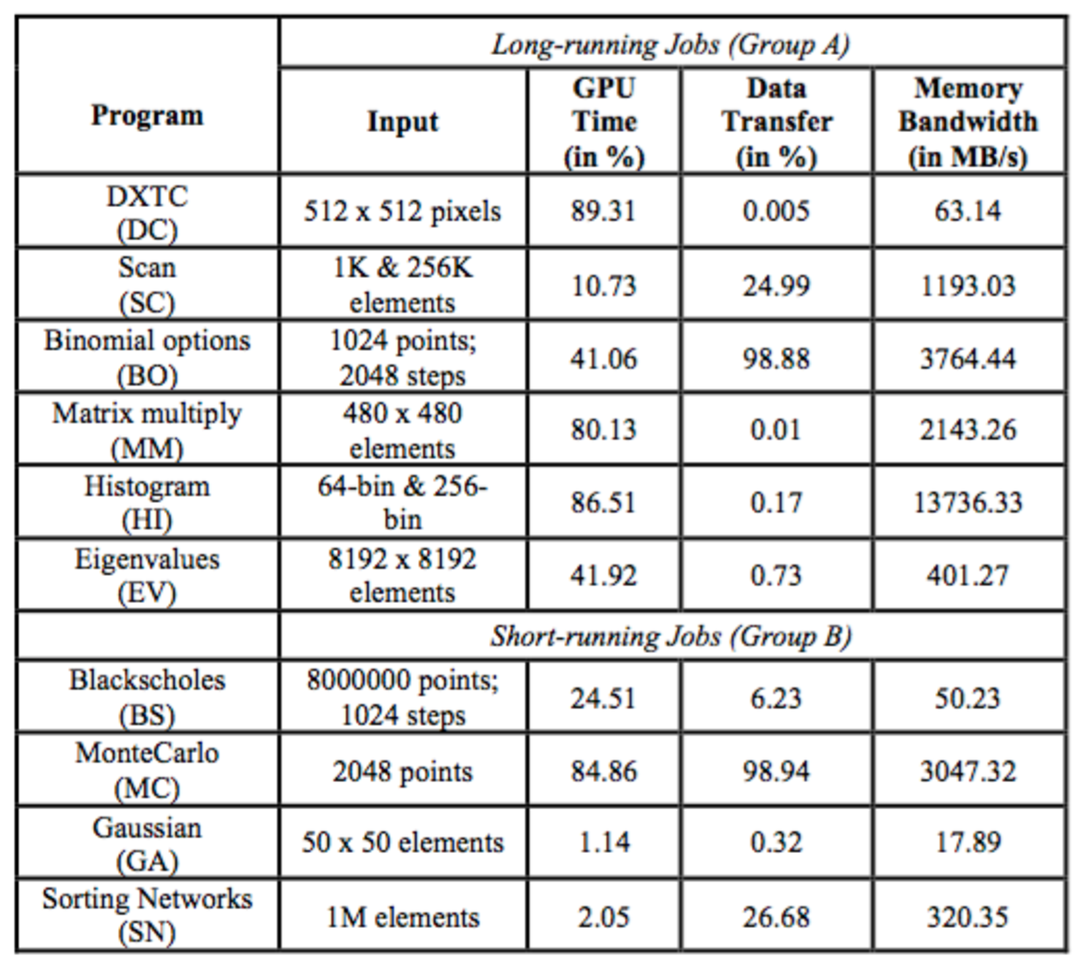
\includegraphics[width=0.9\textwidth,height=\textheight,keepaspectratio]{figures/Strings_Table.pdf}
%\vspace{-0.5cm} 
\end{table*}

\begin{figure}[t]
\centering
%\includegraphics[width=3.2 in]{figures/cloud-workload.pdf}
\includegraphics[width=0.80\textwidth,height=\textheight,keepaspectratio]{figures/servicemodel.pdf}
\caption{GPGPU application service model following a negative exponential distribution of request arrival from multiple end users.}
\label{fig:servicemodel}
%\vspace{-1\baselineskip}
\end{figure}
\section{Experimental Evaluation}
The purpose of the experimental evaluations shown below is twofold. First, they show the importance of explicit accelerator scheduling for the cloud and server workloads seen in future datacenter systems. Second, device-level feedback about application characteristics and behavior is shown to be critical for obtaining high throughput and efficiently utilizing accelerator resources.
\subsection{Evaluation Metrics}
We use weighted speedup~\cite{dean} and Jain's fairness~\cite{jain} as metrics to measure overall system throughput and fairness, respectively. Weighted speedup measures the average speedup in an application when running alone compared to when the application  is sharing the GPU. The  fairness  metric  measures per-application fairness achieved when two or more applications share the GPU where each is allocated a pre-defined share of the resource.
\begin{equation}
Weighted\  Speedup = \frac{1}{N}*\sum_{i=1}^{N}\frac{T_i^{alone}}{T_i^{shared}} 
\end{equation}

\begin{equation}
Jain's\ Fairness = \frac{(\sum_{i=1}^N\frac{T_i}{W_i})^2}{N*\sum_{i=1}^N(\frac{T_i}{W_i})^2}
\end{equation}
\subsection{Benchmarks}
Applications from the CUDA SDK and the Rodinia benchmark suite~\cite{rodinia}, listed in Table~\ref{tbl:table}, are chosen to create a pairwise workload mix of short ($<$ 10sec) and relatively long (10-55 sec) running jobs. 24 such workload pairs are used, labeled from A to X, where A is the DC-BS pair, B is the DC-MC pair, X is the EV-SN pair, and so on, following the order in Table~\ref{tbl:table}. We assume typical cloud services to operate in response to end user requests, with each individual service running for some small amount of time to complete a single request, but with the requirement of being highly responsive. This assumption matches the service behavior reported by Amazon, for instance, for its web service infrastructure. However, the actual types of service instances being used will vary, which we reflect by carefully choosing for the evaluation a diverse set of application kernels, like image processing (e.g., matrixmult), financial (e.g., BlackScholes), etc. The outcome is a workload mix with many short running rather than a few long running sets of jobs.

\subsection{Experimental Setup}
Experiments are performed on two different classes of servers, a small-scale (two GPUs) server and a higher end (four GPUs) server emulated by a supernode comprised of two dedicated dual-GPU nodes (NodeA and NodeB) connected via Gigabit Ethernet. Each of the two machines is equipped with two Intel Xeon X5660 processors running at 2.8 GHz, for a total of 12 cores and 12 GB of RAM, and has two attached NVIDIA FERMI GPUs. NodeA has a Quadro 2000 and Tesla C2050, while NodeB has Quadro 4000 and Tesla C2070 GPUs, resulting in a supernode with a heterogeneous GPU pool where GPUs differ in terms of their compute and memory bandwidth capacities. The CUDA runtime and driver versions are 5.0 and 319.49, respectively. Our GPGPU application service model, as shown in Figure~\ref{fig:servicemodel}, is based on the SPECpower\_ssj2008 benchmark~\cite{spec}, which models a server application with a large number of end users. User requests follow a negative exponential distribution and are served by a finite  number  of  server  threads. The  exponential distribution models intermittent periods of bursts of load when application requests queue up while  other  requests are being processed, followed by  periods of  calm  when  the  accumulated  requests  are  serviced.  For a particular random stream of requests, the inter-arrival time between any two consecutive requests, can be calculated using the following formula:  
\begin{equation}
T = - \lambda*log(X)
\end{equation}
where $\lambda$ is the mean inter-arrival time between consecutive requests, and $X$ is a random number in the range (0.0, 1.0].

NodeA and NodeB are servers processing GPU application requests. In our small-scale server experiments, NodeA sees a stream of requests following a negative exponential distribution, as described above, with λ proportional to the application’s runtime. In the emulated high-end server experiments, each node sees independent random streams of requests. In both the small and large-scale server experiments the assumption is λ is large enough to handle the memory pressure on GPUs being shared, in other words GPU requests never pile up to the degree that they run out of device memory.
\begin{figure}[t]
\centering
%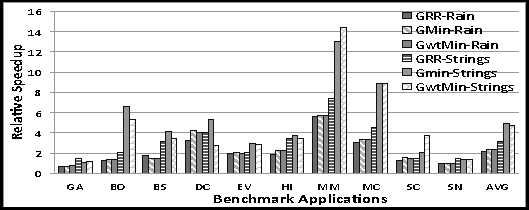
\includegraphics[width=3.2 in]{figures/strings_exp1.pdf}
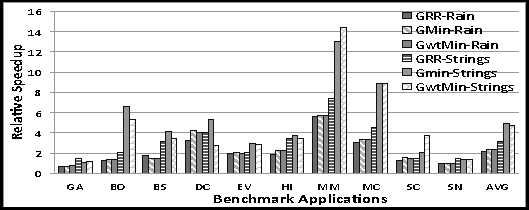
\includegraphics[width=0.75\textwidth,height=\textheight,keepaspectratio]{figures/strings_exp1.pdf}
\caption{Performance benefit of workload balancing policies vs. CUDA runtime in a single node with 2 GPUs.}
\label{fig:strings_exp1}
%\vspace{-1\baselineskip}
\end{figure}


\subsection{Results}
\textbf{Importance of Workload Balancing. }In this set of experiments with a small-scale server, a node receives a stream of requests for a particular application following a negative exponential distribution. As shown in Figure~\ref{fig:strings_exp1}, the average completion time of all requests served is calculated and compared with the different workload balancing policies of Rain and Strings with the baseline being CUDA runtime (relative speedup). We can observe that there is significant throughput improvement with both our former solutions, Rain, and also with Strings, because unlike the CUDA runtime, which respects the application’s target GPU selection, the workload balancer ignores it and dynamically distributes GPU requests across all GPUs in a node. This keeps both of the GPUs in the node busy, avoiding static GPU request collisions, thereby increasing the overall GPU utilization and achieving high system throughput. We also observe that every Strings workload balancing policy performs better than its Rain counterpart. This is because applications mapped to any GPU by Strings belong to the same GPU context and are dispatched over independent CUDA streams. This promotes concurrent execution (1) via time and space sharing the GPU and (2) by keeping both compute and memory copy engines of the GPU busy simultaneously. Averaged over all benchmark applications, the GRR-Rain, GMin-Rain, GWtMin-Rain, GRR-Strings, GMin-Strings and GWtMin-Srings policies achieve weighted speedups of 2.16x, 2.37x, 2.34x, 3.10x, 4.90x, and 4.73x,  respectively,  compared  to the CUDA runtime. Further, on average, Strings workload balancing performs up to 2.10x better than Rain. Interestingly, for some applications (BO, BS and DC), note that GMin outperforms GWtMin, although the latter is, in principle, a better scheduling policy. This is because the static GPU weights assigned to each GPU during system initialization, in many cases, do not mirror the actual relative differences in application performance and therefore, fail to account for diverse application characteristics. This is a  key motivation for feedback-based  load  balancing  evaluated later. In   Strings, for   the   workloads   Gaussian   and  Scan,  GRR performs better than GMin, which seems counter-intuitive. This happens because unlike Rain, in Strings, the per-GPU request queue length (used in the logic of the GMin policy) does not exactly capture the current load in the device. In Rain, the product of queue length and average application runtime in the queue is the total time for servicing the entire queue, but this is not true in Strings, with its multiple GPU requests serviced concurrently. 
\begin{figure}[h]
\centering
%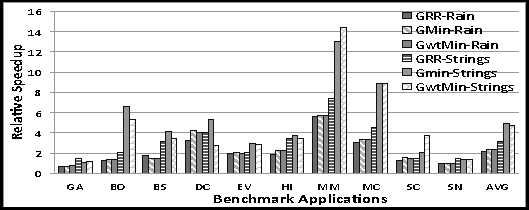
\includegraphics[width=3.2 in]{figures/strings_exp1.pdf}
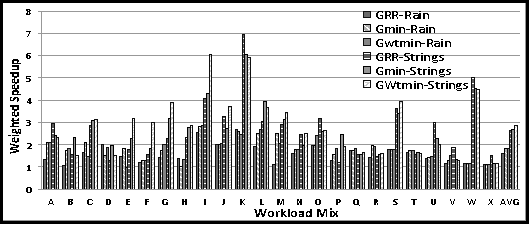
\includegraphics[width=0.75\textwidth,height=\textheight,keepaspectratio]{figures/strings_exp2.pdf}
\caption{Performance benefit of GPU sharing in an emulated 4 GPU server. }
\label{fig:strings_exp2}
%\vspace{-1\baselineskip}
\end{figure}
\begin{figure}[h]
\centering
%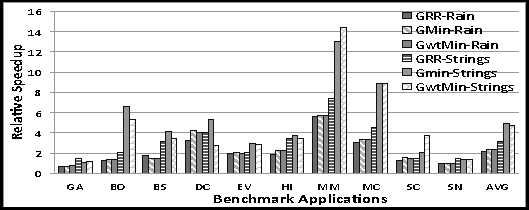
\includegraphics[width=3.2 in]{figures/strings_exp1.pdf}
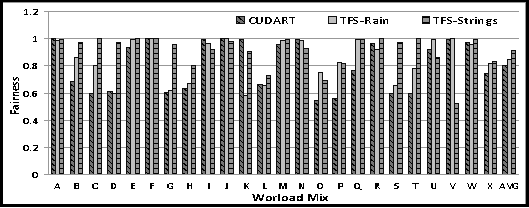
\includegraphics[width=0.75\textwidth,height=\textheight,keepaspectratio]{figures/strings_exp3.pdf}
\caption{Fairness achieved by TFS-Strings vs. TFS-Rain vs. CUDA runtime. }
\label{fig:strings_exp3}
%\vspace{-1\baselineskip}
\end{figure}

\textbf{Benefits of GPU Sharing.} Experiments with the emulated (two node) larger-scale server machine show the benefits of sharing GPUs among multiple application streams. In these experiments, one node receives a stream of longer running GPU requests (Group A) whereas the other receives a stream of shorter requests (Group B), for two different applications and following a negative exponential distribution. Leveraging the gPool, for these sets of requests, the workload balancer dynamically distributes them across all four GPUs in the supernode. Experiments record the average completion time of each application for each of the different workload balancing policies, with the baseline being the single node GRR policy. This means that the performance benefits reported are over and above those obtained with the single node GRR policy described in the previous section. As shown in Figure~\ref{fig:strings_exp2}, averaged over 24 workload pairs, taking one each from Group A and B, the speedups achieved by GRR-Rain, GMin-Rain, GWtMin-Rain, GRR-Strings, GMin-Strings, and GWtMin-Strings policies are 1.60x, 1.80x, 1.82x, 2.64x, 2.69x and 2.88x respectively. These speedups include the effects of both GPU sharing and workload balancing. These notable speedups are derived in part from the fact that the peaks in GPU requests from the two statistically independent streams are not aligned, thus allowing the workload balancer to distribute GPU requests efficiently among all four GPUs. We also observe that for all of the application pairs, maximum speedups are achieved in workloads (I, K and W) in which one of the applications is either BlackScholes or Gaussian. This is because for both of these benchmarks, relative GPU usage is among the lowest,  thus benefiting the other application in the workload mix. Namely, BlackScholes has the least total execution time while the Gaussian kernel has very low GPU utilization, minimal data transfer, and negligible memory bandwidth. Finally, Strings outperforms Rain in GPU sharing because (i) the effect of GPU sharing becomes even more prominent with the opportunity of concurrent execution of GPU requests, and (ii) as shown in the motivation section, a consolidated single GPU context per device makes GPU usage much more uniform, allowing the efficient collocation of multiple requests.

\textbf{Benefits of GPU Scheduling. }We next evaluate a fairshare (TFS) and two throughput-oriented (LAS and PS) GPU scheduling policies.

\textit{1) Fairshare  Scheduler: } in  this  set  of single node experi- ments,  application  pairs  share  a  single  GPU,  each  assigned equal GPU shares. From Figure~\ref{fig:strings_exp3}, we see that TFS-Strings outperforms both the CUDA runtime and the TFS-Rain scheduling policy. The average fairness achieved by TFS- Strings is 91\%, which is 13\% and 7.14\% better than the CUDA runtime and TFS-Rain, respectively. The maximum fairness achieved by TFS-Strings is close to ideal  (99.99\%), for the following reasons. By keeping a history of the GPU time attained by individual applications and penalizing any application in subsequent epochs that used the GPU for more than its allocated share in a previous epoch, both TFS-Rain and TFS-Strings  achieve  better  fairness  compared  to  the CUDA runtime. TFS-Strings achieving higher fairness compared to TFS-Rain might seem counter-intuitive, because the concurrently executing GPU requests from different applications in  Strings  makes  it  difficult  to  track or control fairness in GPU allocation. Better fairness in TFS-Strings can be explained by the fact that because there is no GPU context-switching among applications sharing a GPU in Strings, the error in the calculation of GPU usage of an application in a particular epoch is substantially reduced compared to that of Rain where the GPU context-switching overhead is included in the fairness calculation along with the application’s actual GPU usage.
\begin{figure}[t]
\centering
%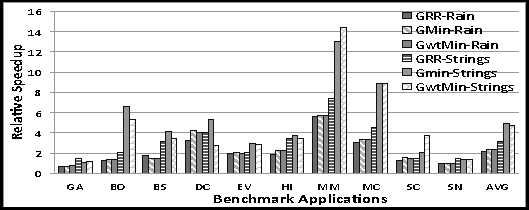
\includegraphics[width=3.2 in]{figures/strings_exp1.pdf}
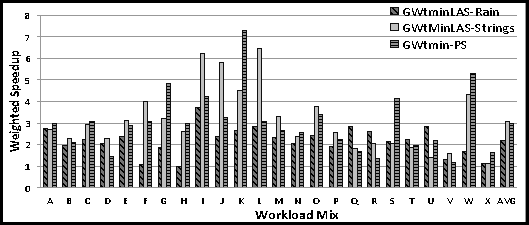
\includegraphics[width=0.75\textwidth,height=\textheight,keepaspectratio]{figures/strings_exp4.pdf}
\caption{Performance benefit of GPU scheduling. }
\label{fig:strings_exp4}
%\vspace{-1\baselineskip}
\end{figure}
\begin{figure}[h]
\centering
%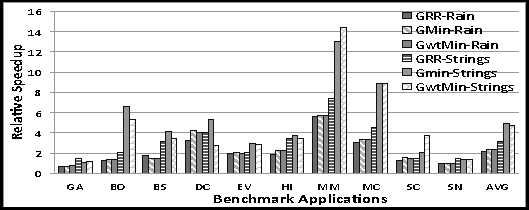
\includegraphics[width=3.2 in]{figures/strings_exp1.pdf}
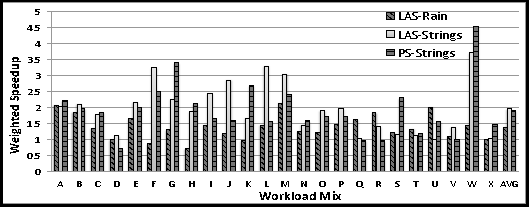
\includegraphics[width=0.75\textwidth,height=\textheight,keepaspectratio]{figures/strings_exp5.pdf}
\caption{Performance benefit of GPU scheduling policies.}
\label{fig:strings_exp5}
%\vspace{-1\baselineskip}
\end{figure}

\textit{2) Throughput Oriented Scheduler: } the baseline for this set of experiments is again the single node GRR policy, and scheduling policies are evaluated in combination with the best performing workload balancing policy from GPU sharing, i.e. GWtMin. As shown in Figure~\ref{fig:strings_exp4}, the average weighted speedup achieved with GWtMinLAS-Rain, GWtMinLAS-Strings, and GWtMin-PS is 2.18x, 3.10x, and 2.97x, respectively. The higher speedup achieved by LAS is because it greedily prioritizes the GPU requests that have shorter GPU episodes and have consumed less GPU time until the most recently completed scheduling epoch. This helps in completing the short running GPU jobs faster and thus increasing the overall system throughput. PS is a Strings-only scheduling policy specifically designed to leverage the concurrency opportunity exposed by CUDA streams and tries to keep all the hardware units in a GPU busy by favoring applications which are in different phases of their use of the GPU, to be active simultaneously. Although it slightly falls short in comparison to GWtMinLAS-Strings, by just 4\%, it does significantly better than   GWtMinLAS-Rain,   by   almost   27\%.   Therefore,   PS achieves  nearly  the  same  throughput  as  LAS  but  is  not  as unfair as LAS, which is an extremely greedy policy by definition and thus, might starve applications with relatively longer GPU episodes. The performance benefits shown in Figure~\ref{fig:strings_exp4} include the effect of both GPU sharing and device level GPU scheduling. To depict solely the benefits of GPU scheduling, Figure~\ref{fig:strings_exp5} compares the GPU scheduling policies with the baseline of GRR policy with four GPUs shared.  LAS-Rain, LAS-Strings and PS-Strings achieve 1.40x, 1.95x and 1.90x throughput improvement respectively over this baseline.

\textbf{Importance of Device-level Feedback.} Feedback-based policies are evaluated relative to the single node GRR policy. When the workload  balancer  receives  feedback  information from low-level GPU schedulers, it dynamically switches to the appropriate  feedback-based  load  balancing policy.  Figure~\ref{fig:strings_exp6} shows the weighted speedup achieved by two feedback-based policies, RTF and GUF, for both Rain and Strings. Average speedups attained are 2.22x, 2.51x, 3.23x, and 3.96x for RTF-Rain, GUF-Rain, RTF-Strings, and GUF-Strings, respectively. Compared to the highest speedup achieved by the previously discussed non-feedback based policy (GWtMinLAS-Strings), RTF-Strings and GUF-Strings achieve 4.5\% and 28\% improvements, respectively. Feedback-based policies outperform static workload balancing, because they make use of more detailed information about application characteristics. E.g., unlike GWtMin, which is a proactive scheduling policy that relies on static weights assigned to GPUs, RTF employs a reactive scheduling technique that uses the actual GPU-specific runtimes of applications to balance load. GUF outperforms RTF in the workload mix of applications that have widely contrasting GPU utilization, i.e., pairs with very high (DC, HT, MM and BO in Group A) and very low (Gaussian, SN and BS in Group B) GPU utilization, by not collocating multiple applications with high GPU utilization on the same GPU.
\begin{figure}[t]
\centering
%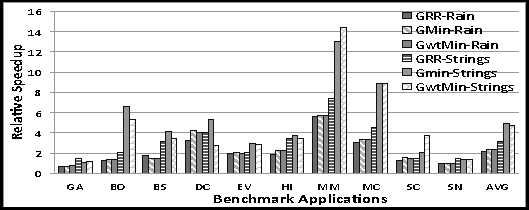
\includegraphics[width=3.2 in]{figures/strings_exp1.pdf}
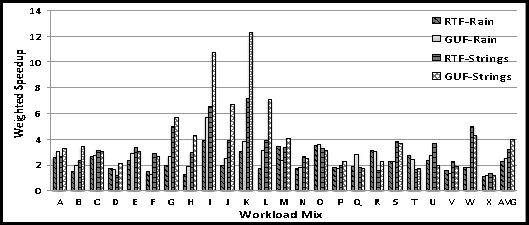
\includegraphics[width=0.75\textwidth,height=\textheight,keepaspectratio]{figures/strings_exp6.pdf}
\caption{Performance benefit of feedback-based load balancing.}
\label{fig:strings_exp6}
%\vspace{-1\baselineskip}
\end{figure}
\begin{figure}[t]
\centering
%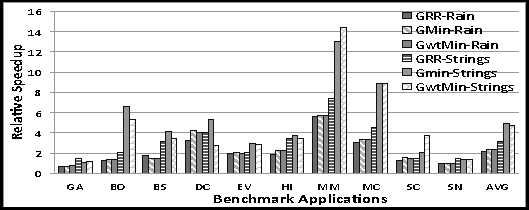
\includegraphics[width=3.2 in]{figures/strings_exp1.pdf}
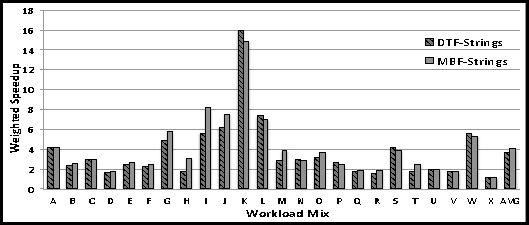
\includegraphics[width=0.75\textwidth,height=\textheight,keepaspectratio]{figures/strings_exp7.pdf}
\caption{Performance benefit of two Strings specific feedback-based load balancing policies.}
\label{fig:strings_exp7}
%\vspace{-1\baselineskip}
\end{figure}

Finally, we evaluate two Strings-specific feedback policies, DTF and MBF, which are designed to exploit the advantages offered by CUDA streams and context packing. As shown in Figure~\ref{fig:strings_exp7}, DTF and MBF achieve average speedups of 3.73x and 4.02x, respectively.  DTF performs best in a workload mix of applications with contrasting degrees of data transfer demands and GPU compute times, i.e., application pairs that have high GPU compute times (DC, EI, HT and MM in Group A) and high data transfer times (MC and SN in Group B). So, when one application is busy in data transfer to the device, the other can continue to use the device for computation. MBF, which is the best performing feedback-based policy, optimally performs in the workload mix of applications with sufficient asymmetry in their memory access behavior, i.e., application pairs with high GPU compute time but low memory bandwidth (EV and DC in Group A) and with high memory bandwidth (BS, HI and MC in Group B). This allows a higher degree of parallelism, by hiding the long memory latencies of memory-bound applications via a runtime switch to a compute-bound application. It is also important to note that by definition, MBF includes the benefits of both RTF and DTF, because the methodology to calculate the approximate memory bandwidth (the ratio of the total data accesses by its computation kernels to the total time spent in the GPU) includes both the data transfer and running time information of the application. This makes MBF perform better than RTF and GUF, across almost all workload mixes. MBF performs better than GWtMinLAS-Strings, RTF, and GUF by more than 30\%, 24\%, and 1.5\% respectively. Therefore, the maximum weighted speedup achieved across all the policies is 4.02x (MBF) relative to single node GRR policy, and 8.70x compared to the bare CUDA runtime.       

\textbf{Discussion. }Key insights from the experimental results in this section are the following. (1) GPU underutilization due to static collisions is avoided by making GPUs into explicitly scheduled entities, thus enabling the load balancing of GPU requests over an aggregated shared GPU pool (gPool). The outcome is an average speedup of up to 4.90x compared to the CUDA runtime. (2) GPU core idling can be reduced further by packing the GPU components of applications sharing a GPU into a single GPU context, causing improvements over schedulers without this ability of an average 2.10x for representative server workloads. (3) Fine-grain feedback from device-level scheduling to load balancing is important, as demonstrated by the fact that GMin performs better than GWtMin for some applications, despite the latter policy’s theoretical superiority. More generally, feedback policies outperform other workload balancing methods, achieving an average speedup of 8.70x. This is because they better understand application characteristics and can thus maximize GPU utilization by collocating applications with contrasting behavior in terms of data transfer and memory intensity. (4) Substantial advantages can be derived from collocating on the same device, streams of requests with likely unaligned peak performance demands, resulting in more uniform GPU usage patterns. Such uniformity is further encouraged by context packing and the consequent sharing of GPU context. (5) An important outcome of this work is that scheduling must go beyond considering GPU resources to also consider other schedulable device components, i.e., the GPU’s data movement engines. This is shown by the phase selection policy leveraging CUDA streams to keep all hardware units in a GPU busy. It achieves system throughput of 6.41x over the CUDA runtime, and it performs as well as the greedy, unfair LAS policy, but without compromising fairness.

\section{Related Work}
From the existing body of work on heterogeneous schedulers, StarPU~\cite{starpu} and Symphony~\cite{symphony} employ a dynamically learned performance model to decide which of the available resources to use, assuming optimized implementations of the same application targeted to different resources exist and can be dynamically dispatched to any one of them as needed. Previous work on interference-driven GPU resource management~\cite{phull} aims to provide better GPU utilization in heterogeneous clusters, by co-locating multiple jobs to share same GPU, respecting GPU memory constraints, but unlike Strings, which decouples the CPU and GPU components of a job and schedules them separately, ~\cite{phull} schedules both application components together on the same node, which might be restrictive. Further, Strings dynamically learns the application’s GPU characteristics, whereas ~\cite{phull} performs static profiling. 

Recent work~\cite{becchi} on managing GPU memory pressure arising from consolidating multiple applications on a single GPU is an interesting complement to our work. Similar middleware infrastructures have recently been proposed for other heterogeneous architectures like Intel’s Xeon Phi~\cite{phi}. By incorporating the virtual memory support of ~\cite{phi, becchi}, Strings can eliminate the assumption on the maximum rate of request arrivals in GPU servers. Gdev~\cite{gdev} implements open source versions of CUDA driver and the runtime library, using which, unlike [16] which presents its virtual memory abstraction at the runtime API level, it builds virtual memory support for GPUs inside the OS kernel. With the Gdev open source driver, both the context packer module and device-level scheduler of Strings can be pushed inside the OS kernel, eliminating runtime layer overheads. GEMTC middleware infrastructure~\cite{GPU43} implements a dynamic memory management system that efficiently allocates memory on the GPU. But unlike Strings, which is completely transparent to the applications, GEMTC exposes a set of new memory management APIs that require applications to be rewritten. Moreover, Strings supports management of heterogeneous multi-GPU resources on a single node which GEMTC infrastructure is yet to support.

In general, previous work on GPU virtualization GVim~\cite{gvim}, Pegasus~\cite{pegasus}, vCuda~\cite{vcuda}, rCuda~\cite{rcuda}, gVirtus~\cite{gvirtus} make the GPUs visible from within the virtual machine. GVim and Pegasus both do QoS-aware scheduling by using a working queue per GPU, but they do not address the problem of scheduling GPU requests across multiple GPUs within a node or across multiple nodes in a cluster. Pegasus also explores the co-scheduling of GPU request with corresponding VCPUs. This can be combined with our Strings infrastructure by gang scheduling decoupled application's CPU and GPU components. vCuda and rCuda leverage the multiplexing mechanism of the bare CUDA runtime for GPU sharing, but they don't look into scheduling policies targeting various resource management goals. 

\section{Chapter Summary}
This chapter presents the Strings scheduler and scheduling policies for GPUs as first class schedulable entities in high-end cloud services. Decomposing the scheduling problem into a combination of workload balancing and device-level scheduling, Strings contributes scheduling policies that explicitly consider data movement to/from accelerators, methods that dynamically encapsulate the GPU contexts of multiple applications into a single umbrella context to achieve high GPU utilization and minimize context switching overhead, and support that makes possible the runtime switching of policies based on device-level scheduler feedback. Novel scheduling policies developed with Strings include (i) a Phase Selection (PS) policy that aims to keep all of a GPU’s hardware units busy by smartly picking and simultaneously running applications operating in different phases of their use of the GPU, (ii) advanced feedback-based policies like DTF and MBF that exploit the advantages offered by CUDA streams and context packing, by collocating applications with contrasting behavior, in terms of data transfer and memory intensity, to achieve extreme performance benefits, (iii) a throughput oriented greedy but highly unfair LAS policy favoring jobs with least-attained levels of GPU service, and (iv) history-based fairshare scheduling that improved fairness in GPU usage for multi-tenant applications.

Extensive experimental evaluations across a wide variety of workloads and system configurations shows Strings to achieve speedups of up to \textbf{4.90x} and \textbf{2.07x} on a single node compared to the CUDA runtime and over our own previous GPU scheduling work, Rain, respectively. Averaged over 24 pairs of short and long running workload mix, Strings achieve a weighted speedup of up to \textbf{8.70x }and \textbf{13\%} improvements in fairness over the CUDA runtime.

Our future work will consider dynamic opportunities and tradeoffs in mapping executions to either GPUs or CPUs, using runtime methods for binary translation~\cite{ocelot}. Also interesting is further exploration of the effects of data movement on program performance and consequent changes in scheduling policies, first for discrete vs. integrated GPUs and second considering GPU multi-tenancy.

%\chapter{Large-Scale Graph Processing using Accelerator-Based System}
%\section{Introduction}
The need to rapidly process large graph-structured data, in both scientific and commercial applications, has engendered
recent efforts to leverage cost-efficient GPUs \cite{Rain, Strings} for efficient graph analytics. Doing so, however, requires
addressing substantial technical challenges, including (1) dealing with the dynamic nature of graph parallelism \cite{medusa, mapgraph, cusha, naila}, (2) coping with limited on-GPU memory, i.e., to process graphs with memory footprints
that exceed limited GPU memory sizes \cite{chi, xstream}, and (3) addressing programmability issues for developers with limited
insights into how to best exploit the resources of evolving and varied GPU architectures \cite{ppl,pact,jure}.

Previous work on parallel graph processing has sought to exploit scale-out methods, by distributing
large graph data across the different nodes of computational clusters \cite{graphlab}. Recognizing the low computation to 
communication ratios of typical graph processing algorithms \cite{chi,xstream}, the `GraphReduce' (GR) programming
framework presented in this chapter uses the alternative `scale up' approach in which large graphs processed 
by memory-limited GPUs can take advantage of the potentially considerable memory capacities of the host machines 
to which they are attached. The implementation of GR for NVIDIA GPUs evaluated in this chapter efficiently runs 
irregular graph algorithms on datasets considerably larger than GPU memory sizes, by (i) partitioning graphs into
fixed size chunks -- shards -- asynchronously moved between GPU and host, (ii) adopting a combination of 
of edge-(X-Stream \cite{xstream}) and vertex-(GraphChi \cite{chi}) centric implementations of graph representations,
(iii) overlapping GPU computation with data transfer via concurrent GPU operations, using CUDA streams, and 
(iv) using `spray' operations to further divide shards and obtain fine-grain parallelism that exploits the 
Hyper-Q feature of Kepler GPUs \cite{kepler}. Specifically, spray operations are used to further divide each shard into multiple 
sub-buffers transferred over dynamically created CUDA streams. The purpose is efficiently use GPU hardware features
like Hyper-Qs.

GraphReduce runs graph algorithms on GPUs without unduly burdening graph algorithm developers. 
Programmers write the appropriate sequential codes for their algorithms, e.g., for data mining, machine learning, etc.,
and then use its simple API to express their use for processing entire graphs. The GR runtime partitions the
graph into different shards, each single one of which entirely fits into GPU memory. Graph processing, then, 
overlaps shard movement with GPU-level graph processing, the latter using multiple levels of GPU-level parallelism,
as indicated above. With such automation, GR can deal with graph sizes much exceeding GPU memory sizes. This is
important because even a common Yahoo web-graph comprised of 1.4 billion vertices \cite{yahoo} requires approximately 
6.6 GB of memory to store just its vertex values (not even including the edges and their status). 

In summary, with GraphReduce, GPUs can be used to accelerate analytics performed on graphs with billions of edges, 
operating at speeds much exceeding that of similar operations run on CPUs, and programmed in ways accessible 
to programmers who are not experts in GPU programming. To the best of our knowledge, GraphReduce is the first
to support in-GPU-memory and out-of-GPU-memory graph processing, thus aiming for scale-up graph processing 
on HPC systems with discrete GPUs and high end (i.e., memory-rich) hosts.

\section{Background and Motivation}
\label{bg}

This section introduces the computational model used in GraphReduce. It also motivates the GR approach by describing some of
the challenges faced by the existing state-of-the-art graph processing approaches.

%\vspace{-0.5\baselineskip}

\subsection{Computational Model: GAS Abstraction}


\begin{figure}[!t]
\centering
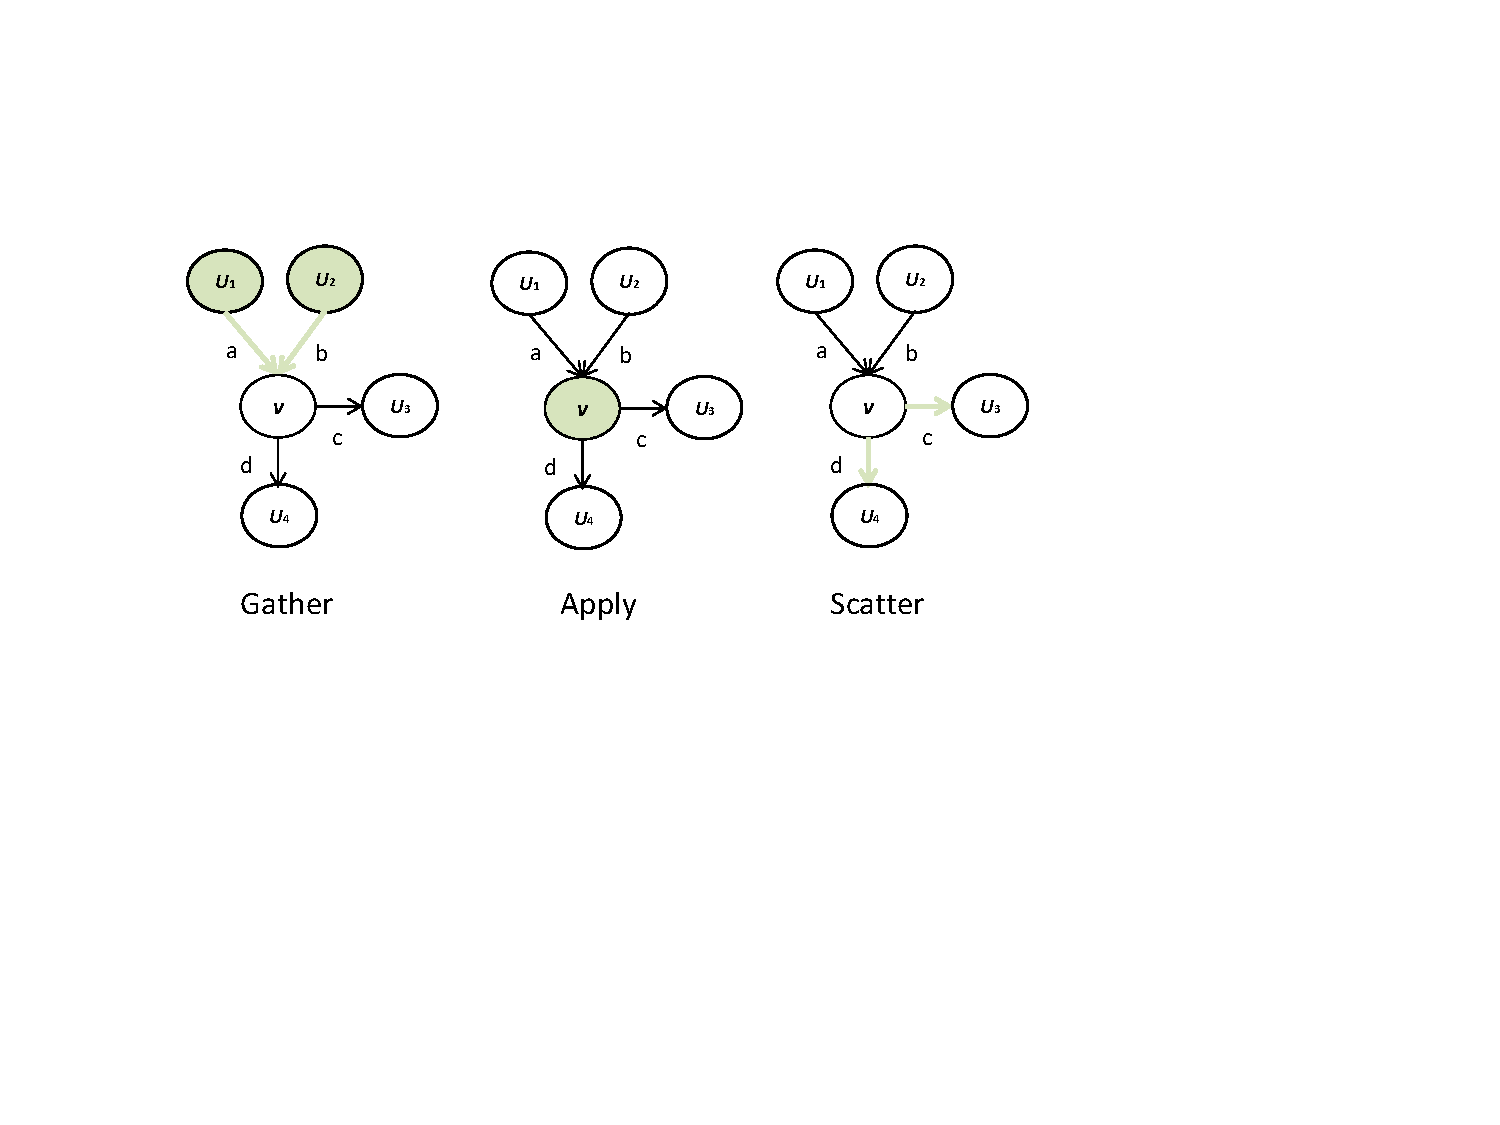
\includegraphics[width=0.9\textwidth,height=\textheight,keepaspectratio]{figures/phases.pdf}
\caption{An example of GAS abstraction. }
\label{fig:phases}
%\vspace{-1\baselineskip}
\end{figure}


GraphReduce exposes the Gather-Apply-Scatter (GAS) computational model used by Pregel \cite{pregel}, Powergraph \cite{powergraph}, and GraphLab \cite{graphlab}.
With GAS, a problem is described as a directed (sparse) graph, $G = (V, E)$, where $V$ denotes the vertex set and $E$ denotes 
the directed edge set. A value is associated with each vertex $v\in V$, and each directed edge $e_{ij}$ is associated with 
a source vertex $u$ and a target vertex $v$: $e_{ij} =(u, v) \in E$. Given a directed edge $e_{ij} = (u, v)$, we refer to 
$e_{ij}$ as vertex $v$'s in-edge, and as vertex $u$'s out-edge. A typical GAS computation, then, has three stages \cite{vertexapi}: 
(1) Initialization, (2) Iterations, and (3) Output. Initialization deals with initializing vertex/edge values and a starting 
{\em computation frontier}, which is defined as the set of active vertices for a given iteration. In each Iteration stage, 
a sequence of iterations is run, each gathering the values seen on the incoming edges, updating the values of elements, and 
then defining a new frontier for the next iteration. Figure \ref{fig:phases} illustrates these three phases, assuming vertex $v$ to be the 
central vertex.


%\vspace{-0.5\baselineskip}
\begin{itemize}
  \item {\bf Gather Phase}: each vertex aggregates values associated with its incoming edges and their source vertices. 
We define the gather function as $G(u, v, e_{ij})$, and we use binary operator $\biguplus$ to aggregate the outputs 
from multiple $G$s into one value $R$. In Figure 1 (a), the result ($R$) from the Gather Phase for vertex $v$ can be represented 
as $R= G(u_1, v, a)\biguplus G(u_2, v, b)$. 
 % \vspace{-0.5\baselineskip}
  \item {\bf Apply Phase}: the value of each vertex in the current frontier is updated through the gather result. 
We define the update function as $U(v, R)$, where $R$ is the result from the Gather Phase. Shown in the Figure 1 (b), 
we have the updated vertex $v$ as: $v' = U(v, R)$.  
 % \vspace{-0.5\baselineskip}
  \item {\bf Scatter Phase}: the new vertex state is propagated to neighbors, by updating the state of its out-edges 
(e.g., $c$ and $d$ in Figure 1). We define the Scatter function for updating the out-edges of $v$ as $S(v', e_{out})$, 
where $v'$ is the updated vertex $v$ and $e_{out}$ represents $v$'s out-edges. Shown in Figure 1 (c), two updated edges 
$c'$ and $d'$ are denoted as: $c' = S(v', c)$ and $d' = S(v', d)$.
%\vspace{-0.5\baselineskip}
\end{itemize} 


As shown in much prior work \cite{powergraph, pregel, sc05}, the GAS model is not only simple to use, but it is also sufficiently general to express
a broad set of graph algorithms, ranging from PageRank to Connected Components, and from Heat Simulation to Sparse Linear Algebra. 
For example, the PageRank algorithm \cite{pagerank} can be expressed as follows. In the {\bf Gather Phase}, each vertex $v_i$ in the current 
frontier accumulates $G_i = \sum_{}^{}{\frac{R_j}{n_j}}$ from all in-edges from source vertex $v_j$, where $R_j$ is the rank of 
$v_j$ and $n_j$ is the number of out-edges ($v_j\rightarrow v_i$) of $v_j$. Then, in the {\bf Apply Phase}, vertex $v_i$ updates 
its value using some common PageRank formula like $R_i = 0.85+0.15\times G_i$. Since in PageRank, the values of out-edges of 	$v_i$ will not change 
in the {\bf Scatter Phase}, there are no operations for this phase. 


\begin{figure}[!t]
\centering
\includegraphics[width=\textwidth,height=\textheight,keepaspectratio]{figures/hybrid-model.pdf}
\caption{ (a) Vertex-centric Scatter-Gather. (b) Edge-centric Scatter-Gather. }
\label{fig:vertex-edge}
%\vspace{-1\baselineskip}
\end{figure}




Figure \ref{fig:vertex-edge} shows two common ways to implement graph algorithms with GAS: edge-centric vs. vertex-centric execution, which differs in whether the
Scatter and Gather phases iterate over and update edges or vertices (their pseudo codes are shown in Figure \ref{fig:vertex-edge}).
Implementation can also vary in terms of Update functions, to be implemented as either Bulk-Synchronous Parallel (BSP) \cite{BSP}
for simplicity or via asynchronous execution, for faster convergence. In either case, the graph algorithm terminates
when some application-specific condition is met, e.g., when no more changes in vertex and edge states beyond a certain threshold. 


\subsection{Motivation and Challenges}

\begin{table}[h]%\scriptsize
\centering
\begin{tabular}{lllc}
Graph Name & Vertices & Edges & \multicolumn{1}{l}{In-memory Size} \\ \hline
\multicolumn{4}{c}{GPU In-Memory} \\ \hline
ak2010\cite{ak2010}& 45,292 & 108,549 & 7.9MB \\
coAuthorsDBLP\cite{coauthors} & 299,067 & 977,676 & 69.5MB \\
kron\_g500-logn20\cite{kron20} & 1,048,576 & 44,620,272 & 2.4GB \\
webbase-1M\cite{web} & 1,000,005 & 3,105,536 & 211.6MB \\
belgium\_osm\cite{belgium} & 1,441,295 & 1,549,970 & 5.4MB \\ \hline
\multicolumn{4}{c}{GPU Out-of-Memory} \\ \hline
kron\_g500-logn21\cite{kron20} & 2,097,152 & 91,042,010 & 4.84GB \\
nlpkkt160\cite{nlpktt} & 8,345,600 & 221,172,512 & 11.9GB \\
uk-2002\cite{uk2002} & 18,520,486 & 298,113,762 & 16.4GB \\
orkut\cite{orkut}& 3,072,441 & 117,185,083 & 6.2GB \\
cage15\cite{cage15} & 5,154,859 & 99,199,551 & 5.4GB
\end{tabular}
\caption{ Datasets used to evaluate GraphReduce framework. `Out-of-memory' means that the input graphs cannot fit into the limited GPU memory. A commercial K20c GPU with a 4.8 GB global memory is used as an example to illustrate in-memory and out-of-memory cases.}
\label{datasets}
%\vspace{-0.5\baselineskip}
\end{table}




\begin{table}[h]%\scriptsize
\centering
\begin{tabular}{cccc}
\hline
Graphs & X-Stream (ms) & CuSha(ms) & \multicolumn{1}{l}{Speedup} \\ \hline
ak2010 & 215.155 & 7.75 & 28x \\
belgium\_osm & 2695.88 & 791.299 & 3x \\
coAuthorsDBLP & 1275 & 11.553 & 110x \\
delaunay\_n13 & 80.89 & 5.184 & 16x \\
kron\_g500-logn20 & 46550.7 & 119.824 & 389x \\
webbase-1M & 3909.12 & 13.515 & 290x
\end{tabular}
\caption{Performance comparision between two state-of-the-art graph processing approaches. X-Stream runs on a 16 core Xeon E5-2670 CPU with 32GB memory. CuSha runs on a NVIDIA K20c Kepler GPU with 4.8 GB memory. }
\label{gpu-cpu}
%\vspace{-0.5\baselineskip}
\end{table}


\subsubsection{Why Graph Analytics Using GPUs ?}
The high compute power and multi-level parallelism provided by the SIMT (Single Instruction Multiple Threads) architectures of GPGPUs \footnote{\scriptsize Without specified mention, NVIDIA terminology will be used throughout the chapter
to illustrate our work. However, the proposed methodology can be easily applied to a wide range of massively
parallel architectures.} present opportunities for 
accelerating many graph algorithms \cite{medusa, cusha,vertexapi,mapgraph}. Table \ref{gpu-cpu} shows the performance comparison between two state-of-the-art graph analytics 
processing the BFS algorithm: X-Stream \cite{xstream} for CPUs and CuSha \cite{cusha} for in-memory GPU processing. Significant performance speedups are
observed from using the GPU. For instance,  graph kron\_g500-logn20 \cite{kron20} processed by CuSha on a commercial K20c Kepler GPU 
(4.8GB memory) achieves 390x speedup over X-Stream on a 16 core Xeon E5-2670 CPU (32 GB memory).


\subsubsection{Challenges in GPU Graph Analytics?}
Acceleration of graph analytics via GPUs is limited, however, by the fact that many real-world graphs cannot fit into 
GPUs' limited memories. As mentioned earlier, a common Yahoo-web graph \cite{yahoo} with 1.4 billion vertices requires 6.6 GB memory 
just to store its vertex values. Additional examples of graphs exceeding GPU memory sizes appear in Table \ref{datasets}.
Previous work on GPU-based graph processing has not addressed this issue. CuSha \cite{cusha}, MapGraph \cite{mapgraph}, VertexAPI \cite{vertexapi} and Medusa \cite{medusa} all assume graphs to reside in GPU memory. GraphChi \cite{chi} and X-Stream \cite{xstream} are designed for CPU-based systems, 
unable to benefit from the multi-level massive parallelism offered by GPUs (shown in Table \ref{gpu-cpu}). Hybrid approaches (CPU+GPU) like Totem \cite{totem} are only able to process a fixed sub-graph that can fit into GPU memory after statically partitioning the graph between CPU and GPU, which results in underutilization of GPU's fullest processing power and parallelism. 
 


%Totem \cite{totem} provides a high-level abstraction to address a hybrid environment (CPU+GPUs), 
%by statically partitioning the graphs into GPU and host CPU memories. Specifically, performance improvements are obtained for
%graphs following a power-law vertex distribution by placing low-degree vertices on the CPU and high-degree vertices on the GPU.
%As graph size increases, however, only a fixed sub-graph can fit into GPU memory, leading to diminishing returns for
%such static partitioning, since more and more of the graph processing will be bottlenecked by the slower compute engine (CPU). 




% (\textcolor{red}{/*Figure XX shows examples of large graphs that do not fit in GPU memory and their vertex distributions are not suitable for Totem. I have two graphs of vetex degree %distribution for two large graphs. wait for totem results before adding here /*}). 


\begin{figure}[!t]
\centering
\includegraphics[width=\textwidth,height=\textheight,keepaspectratio]	{figures/frontier.pdf}
\caption{Frontier size changes across iterations using the GAS model on GPUs. This phenomenon highly depends on the input graph and algorithm, showcasing the inherent graph irregularity. Four cases from left to right: (a) Cage15 - PageRank; (b) nlpkkt160 - PageRank; (c) Cage15 - BFS; and (d) orkut - Connected Component (CC). 
 }
\label{fig:frontier}
%\vspace{-0.5\baselineskip}
\end{figure}

\subsubsection{Challenges in Evolving Graph Analytics On GPU}

\begin{figure}[!t]
\centering
\includegraphics[width=0.75\textwidth,height=0.75\textheight,keepaspectratio]{figures/static_GR.pdf}
\caption{State-of-the-art GPU frameworks (i.e., MapGraph, GraphReduce and Cusha) for processing static graphs significantly outperform the best CPU-based framework X-Stream (baseline).}
\label{fig:static}
%\vspace{-0.5\baselineskip}
\end{figure}

GPUs have emerged as one of the most powerful computation accelerators for world-class supercomputers~\cite{titan} because of their unparalleled massive amount of parallelism and ability to speedup a wide range of HPC applications. Compared to its counterpart CPU, it also often provides superior acceleration for general graph algorithms. Figure \ref{fig:static} demonstrates that for processing three real-wold in-memory \textit{static graphs} under BFS, state-of-the-art GPU frameworks outperform the best CPU-based graph analytics (i.e., X-Stream) by an average speedup of 782x and up to 2785x (i.e., GraphReduce on \textit{webbase-1M}). This motivates us to unleash GPU's high computation power for processing \textit{evolving dynamic graphs}. 

Figure \ref{fig:link} shows an example of an evolving Linkedin social network graph, in which a subgraph (circled by red dashed line) is going through \textit{update batches} (e.g., insert:(1,4) and delete:(1,3)) at different time point. Different colors of dots represent work fields. Processing such common constantly-evolving social network graphs on GPUs is very challenging because (i) highly efficient computation model and convenient programming constructs do not exist for programmers to effectively express their algorithms on GPUs, (ii) how to efficiently utilize the parallelism provided by GPUs to deal with the computation and data storage overlap in dynamic graphs is complicated, and (iii) how to extract the most throughput from GPUs without burdening the users with hardware details is unclear. In order to address these challenges, we designed a runtime graph analytics framework named \textit{EvoGraph} to process complex evolving graphs on modern GPUs. Under EvoGraph, users only need to write sequential codes and the sophisticated runtime will seamlessly map the incremental graphs to GPU for acceleration. We will discuss the design details of EvoGraph next. 



\begin{figure}[!t]
%\vskip -3 mm
\centering
\includegraphics [width=1\columnwidth]{figures/link.pdf}
\caption{A subgraph of a Linkedin social network has been updated over time but the rest of the network remains the same. }
\label{fig:link}
%\vspace{-0.5\baselineskip}
%\vskip -3 mm
\end{figure}



There are several challenges to efficiently process larger-than-memory graphs on GPUs. They involve the need to provide end
users with convenient programming constructs for their graph algorithms, but without unduly burdening them with (i) graph partitioning to
fit sub-graphs into GPU memory, (ii) how and when such partitions are moved between GPU and host memories, and (iii) how to best
extract multi-level parallelism from their GPU-resident execution. The GraphReduce framework presented in this chapter 
addresses these challenges.




Graph partitioning or chunking for fitting into GPU memory must deal with the irregular nature of 
graph algorithms and how they access the input data. More specifically, to obtain high on-GPU performance, chunking
must be done to minimize GPU-host data movement. For the GAS model, this requires ensuring GPU memory residence of 
the vertices and edges that actively take part in the computation iterations being performed.
This despite the fact that due to the inherent irregularity in graph algorithms, in every computation iteration, the number 
of edges and vertices that actively take part in computation (computation frontier size) is not constant, and it varies with 
graph algorithms and datasets, as shown in Figure \ref{fig:frontier}. Across all of these cases, the frontier sizes \footnote{\scriptsize The term ``frontier size" is synonymous with the number of active vertices in a given iteration. The variation of the frontier size during execution is sensitive to the starting-point for graph processing. } 
incur significant changes (either dropping or climbing). For instance, in Figure \ref{fig:frontier}(b) for graph nlpkkt160 processed 
by PageRank, the frontier size drops sharply after a few iterations and remains low for the rest of the execution. 
Given these results, ideally, the GR runtime should {\em move sub-graphs to the GPU only if they
contain active vertices and edges}. Otherwise, such movements simply cause unnecessary overhead.
For the same nlpkkt160 case in Figure \ref{fig:frontier}(b), after several iterations, most of the sub-graphs do not have 
active vertices/edges, so there is no need to move those chunks to the GPU. We have found this phenomena to be very common 
across most of the graphs shown in Table \ref{datasets}, for various algorithms. The GR methods presented in this chapter address this issue, along with (ii) and (iii) above.

%EvoGraph
High performance machines are increasingly using GPUs~\cite{15, 16, 17, 18, 19}, to leverage their scalability and low dollar to FLOPS ratios.  As a result, GPUs have become the main compute engines for today’s HPC clusters and supercomputers like Titan in Oak Ridge~\cite{titan}. This trend continues with the move toward exascale machines that are expected to be comprised of millions of accelerator and general purpose cores, whether packaged as `thin' or `fat' nodes. Another recent trend is the gain in popularity of GPU processing in many domains such as social networks, e-commerce, advertising, and genomics. This has motivated the growing interest in large-scale real-world graph processing for both scientific and commercial applications, as well as the recent efforts in accelerator-based graph processing frameworks such as MapGraph~\cite{mapgraph}, Medusa~\cite{medusa}, CuSha~\cite{cusha}, GraphReduce~\cite{GraphReduce}, and so on. An important aspect of real-world graphs, like Facebook friend lists or Twitter follower graphs, is that they are dynamic.  Given the billions of Facebook~\cite{linkbench} users sharing more than 100 billion photos and posts per month, let alone the volume on Twitter~\cite{twitter} or other blogging platforms, there is a huge need to quickly analyze this high velocity stream of graph data. 

However, state-of-the-art graph analytics for dynamic graphs follow a store-and-static-compute model that involves batching these updates into discrete time intervals, applying all of the updates to the total graph, and then rerunning the static analysis.  There is considerable redundancy and inefficiency in this approach to analyzing this \textit{evolving} graph sequence.  Static graph analytics on a single version of the evolving graph, even when leveraging massive amount of parallelism offered by thousands of cores in a GPU, can be very slow due to the extreme scale of many real-world graphs (e.g., one Facebook graph purportedly has a trillion edges~\cite{fb}) and/or because of the complexity of the graph queries that are traditionally both compute and memory intensive. Second, data movement of the entire input graph repeatedly between the host and the GPU over the slow PCIe link can result in substantial overhead, which in turn can overshadow the benefits from the massive parallelism offered by a GPU.  Finally, there are real world graph analytics problems that inherently require soft or hard real-time guarantees, e.g., real-time anomaly detection, disease spreading, etc, and hence can't use the traditional static recomputation model. Beyond just hardware performance, we also note that the skills to write performant GPU code are substantially different from the coding skills that many analysts have learned.  As one can therefore see, the many demands of high velocity graph data, both commercial and scientific, have outstripped the traditional, batched static graph analytics models, even when using GPUs.

To address this, we propose a two-pronged approach to deal with both the performance and programmability challenges. We introduce an accelerator-based incremental graph processing framework called EvoGraph. EvoGraph employs a new variant of  the popular Gather-Apply-Scatter (GAS) programming model, which we call Incremental-GAS (or I-GAS), to incrementally process a batched stream of updates (i.e., edge/vertex insertions and deletions).  The key insight is that I-GAS algorithms are designed to work over a (dynamically determined) sub-graph of the previous version of the evolving graph.  For many popular graph algorithms and real-world graphs, the corresponding I-GAS logic affects only a fractional portion of the graph; this reduction in problem size can result in tremendous performance benefits compared to static recomputation of the graph algorithm on the entire graph.  The modest additions of the I-GAS model to the already-published GAS model interface enable an easy transition of analysts from coding in a static to a dynamic streaming environment.

From a simplistic view, it would seem that incremental methods would always be preferable.  However, there are scenarios when a streamed update may affect a very large portion of the graph, and incremental processing won't help much or may even be worse than static recomputation due to overheads of incremental execution. One such counterexample is in the incremental version of Breadth First Search (BFS), where updates that affect vertices close to the source/root node will affect nearly the entire BFS tree. Here the incremental run can at best perform as good as the static re-run, and may even be worse. Note that this is not a concern about correctness of the result, but over performance.  Therefore, in order to handle such scenarios, we employ a \textit{per batch}, property-based dynamic choice between incremental and static graph processing called \textit{‘property-guard’}. Utilizing user-defined and built-in properties (e.g., vertex degree) along with programmable control policies, EvoGraph analyzes each update batch and dynamically decides whether to process the graph incrementally using I-GAS or to fall back to static recomputation. 

%\section{Background And Motivation}


%Related Work
\section{Related Work}

{\bf In-Memory Graph Processing.} Merrill \textit{et al.}\cite{Merrill} present 
a parallelization of BFS tailored to the GPU's requirement for large amounts of fine-grained BSP; they achieve an asymptotically 
optimal $O(|V|+|E|)$ work complexity. 
Hong \textit{et al.}\cite{Hong} propose warp-level load-balancing that defers outliers 
and performs dynamic workload distribution to speed up graph algorithms through heavyweight atomic operations on global memory. 
Duong \textit{et al.} \cite{Duong} conduct detailed GPU-based optimizations for PageRank and achieves significant speedup over 
a multi-core CPU implementation. Chapuis \textit{et al.} \cite{ASSP} provide an algorithmic optimization solution to speedup 
all-pairs shortestpath (APSP) for planar graphs that exploits the massive on-chip parallelism available on GPUs. 
GraphReduce can be extended to implement the algorithm-specific optimizations above and in contrast to such work, it offers
user-level APIs for programming graph algorithms and provides a general framework addressing a wide range of parallel graph algorithms 
and hiding architecture-level optimizations from users.

Concerning frameworks for GPU-based graph processing, earlier work like \textit{Medusha} \cite{medusa} introduces some basic
graph-centric optimizations for GPUs, offering a small set of user-defined APIs, but its performance is not comparable to the
state-of-the-art low-level GPU optimizations. To address this issue, \textit{MapGraph} \cite{mapgraph} and \textit{VertexAPI}\cite{vertexapi}
implement runtime-based programming frameworks with levels of performance that match those seen for low-level specific algorithm optimizations. 
\textit{MapGraph} chooses among different scheduling strategies, depending on the size of the frontier and the adjacency lists 
for the vertices in the frontier. 
It also uses a Structure Of Arrays (SOA) pattern to ensure coalesced memory access. 
\textit{VertexAPI} provides a GAS model-based GPU library, gaining high performance primarily from using the 
ModernGPU \cite{moderngpu} library for load balancing and memory coalescing. \textit{CuSha} \cite{cusha} identifies the shortcomings 
of the state-of-the-art CSR-based virtual warp-centric method for processing graphs on GPUs and in response, proposes G-Shards and 
Concatenated Windows to address its performance inefficiency. All of the approaches above make the fundamental assumption that 
large graphs fit into GPU memory, a restriction that is not present for GraphReduce. As discussed in Section 4.5, GraphReduce 
not only addresses the processing of out-of-memory graphs, but also matches the in-memory performance seen with these state-of-the-art 
approaches, in many cases outperforming them significantly. 

{\bf Out-of-Core Graph Processing.} Out-of-Memory graph processing has been concerned with CPU-based hosts processing graphs 
that do no fit into host memory. \textit{GraphChi} \cite{chi}, for instance, is based on a vertex-centric implementation of 
graph algorithms where graphs are sharded onto the SSD drives attached to the host. Its SSD-targeting sharding methods motivate 
GraphReduce's approach to how GPUs view and interact with host memory. (Table \ref{gpu-cpu}). 
GraphChi proposed the concept of partitioning a graph into shards and a novel parallel sliding windows technique to load a subgraph into the CPU memory. This method enables a sequential access of memory as the in-edges are sorted according to their source vertices.  
We also borrow from X-Stream \cite{xstream} the edge-centric way to organize data for our GAS model.
To improve GraphChi with the scenario that large graphs commonly have more edges than vertices, \textit{X-Stream} \cite{xstream} enables an edge-centric scatter-gather model. Unlike GraphChi which requires pre-processing in the form of sorting the in-edges, X-Stream streams unordered edge lists and puts the updates into buckets corresponding to different vertex intervals. Both Graphchi and X-Stream are CPU-based implementations. Although they both have multi-threaded version, they do not come close to the parallelism offered in GPUs which our GraphReduce framework takes advantage of. 
Discussed in Section 4.5.2, GraphReduce enables a hybrid programming model and significantly outperforms state-of-the-art X-Stream for different graph inputs processed by various algorithms. 
\textit{Totem} \cite{totem} offers a high-level abstraction for graph processing on GPU-based systems, by statically partitioning graphs 
into GPU and host memories, placing low-degree vertices on the host and high-degree vertices on the GPU. 
The approach improves performance if the graphs follow a power-law vertex degree distribution, and as graph size increases, only
a fixed sub-graph able to fit in GPU memory will be processed, resulting in GPU underutilization and eventual CPU-based bottlenecks
for graph processing. \textit{Green-Marl} \cite{green} is a Domain Specific Language (DSL) 
for efficient graph analysis on CPUs; its implementation is not amenable to many-core architectures. Also, it requires static analysis to generate thread assignment which will not work for GPU runtime. 

\section{Related Work}

\textbf{Dynamic graph processing.} There are two broad categories of dynamic graphs processing (1) Offline processing of dynamic graphs that involves the generation, storing, and analysis of a sequence of versions or time-stamped snapshots of dynamic graphs for the calculation of some global graph property. (2) Online processing of dynamic graphs that  involve real-time, continuous query processing over streaming updates on the evolving graph. EvoGraph is a framework designed to address the later problem.
Chronos~\cite{chronos}, GraphScope~\cite{graphscope}, and TEG~\cite{teg} are some examples of the most recent work in offline dynamic graph processing. Chronos is a high-performance system that supports incremental processing on temporal graphs using a graph representation that places graph vertex data from different versions together leading to good cache locality. GraphScope proposes encoding for evolving graphs for community discovery and anomaly detection. 

\textbf{Real-time, continuous query processing.} This implies certain memory constraints that might not allow keeping multiple versions of the evolving graph. STINGER~\cite{stinger} defines an efficient data structure to represent streaming graphs that enables fast, real-time insertions and/or deletions to the graph. Several applications have been built using the STINGER graph representation like clustering coefficient [3] and connected components [4]. Unlike STINGER which uses a single data structure for both static and dynamic graph analysis, EvoGraph uses a novel hybrid data structure that allows for incremental computation on edge lists and a compressed format for static graph computation.  A key takeaway of these related work is that any existing algorithm that can be reduced to a GAS-based graph sub-problem can easily leverage EvoGraph to implement their incremental versions.


\textbf{Accelerator-based Graph Processing.}
Merrill et al.[29] present a parallelization of BFS tailored to the GPU’s requirement for large amounts of fine-grained BSP; they achieve an asymptotically optimal $O(|V | + |E|)$ work complexity. Duong et al. [14] conduct detailed GPU-based optimizations for PageRank and achieves significant speedup over a multi-core CPU implementation. Chapuis et al. [13] provide an algorithmic optimization solution to speedup all-pairs shortestpath (APSP) for planar graphs that exploits the massive on-chip parallelism available on GPUs. 	The GraphReduce~\cite{GR} framework can efficiently process graphs with large inputs and mutable edge values that can-not fit into the limited memories of discrete accelerators. The framework characterizes the memory buffers and then maps them to the different memory abstractions exposed by GPU, which at minimum, contain slow and fast memory~\cite{nemu}(e.g., host memory and GPU memory). 		 

Concerning frameworks for GPU-based graph processing, earlier work like Medusha~\cite{medusa} introduces some basic graph- centric optimizations for GPUs, offering a small set of user- defined APIs, but its performance is not comparable to the state-of-the-art low-level GPU optimizations. To address this issue, MapGraph~\cite{mapgraph} and VertexAPI~\cite{vertexapi} implement runtime-based programming frameworks with levels of performance that match those seen for low-level specific algorithm optimizations. MapGraph chooses among different scheduling strategies, depending on the size of the frontier and the adjacency lists for the vertices in the frontier. VertexAPI provides a GAS model-based GPU library, gaining high performance primarily from using the ModernGPU [6] library for load balancing and memory coalescing. CuSha~\cite{cusha} identifies the shortcomings of the state-of-the-art CSR- based virtual warp-centric method for processing graphs on GPUs and in response, proposes G-Shards and Concatenated Windows to address its performance inefficiency. All of the approaches above make the fundamental assumption that large graphs fit into GPU memory, a restriction that doesn't hold true for real-world graphs.

\textbf{Distributed graph processing.} Involves processing of large-scale graphs in a distributed fashion by making use of the combined memories of multiple machines to fit large graphs that don’t fit in a single machine. Pregel~\cite{pregel} provides a synchronous vertex-centric graph processing framework that is based on message passing. GraphLab~\cite{graphlab} provides a framework for machine learning and data mining while PowerGraph~\cite{powergraph} exploits the power-law vertex degree distribution for efficient data placement and computation. ASPIRE~\cite{aspire} adopts an asynchronous mode of execution with a relaxed consistency to improve the remote access latency. These project are complimentary to GraphIn, in that they could be used to implement the static component of GraphIn  computation while I-GAS can be leveraged to make these distributed frameworks more dynamic. 


\textbf{Out-of-Memory graph processing.} Out-of-Core graph processing has been concerned with CPU-based hosts processing graphs that do no fit into host memory. GraphChi~\cite{chi}, for instance, is based on a vertex-centric implementation of graph algorithms where graphs are sharded onto the SSD drives attached to the host. X-Stream~\cite{xstream} employ an edge-centric way to organize data for the GAS model. Totem~\cite{totem} offers a high-level abstraction for graph processing on GPU-based systems, by statically partitioning graphs into GPU and host memories, placing low- degree vertices on the host and high-degree vertices on the GPU. The approach improves performance if the graphs follow a power-law vertex degree distribution, and as graph size increases, only a fixed sub-graph able to fit in GPU memory will be processed, resulting in GPU underutilization and eventual CPU-based bottlenecks for graph processing. Green-Marl~\cite{green} is a Domain Specific Language (DSL) for efficient graph analysis on CPUs; its implementation is not amenable to many-core architectures.
Involves large-scale graph processing in a single machine with graphs that might not fit into host memory. GraphChi~\cite{chi},  X-Stream~\cite{xstream} are two of the recently proposed out-of-memory frameworks. GraphChi is based on a vertex-centric implementation of graph algorithms where graphs are sharded on SSD drives attached to the host while X-Stream uses an edge-centric way to organize data for GAS model. As EvoGraph is framework independent, these out-of-memory frameworks can be used as the static graph processing core for our framework.



\chapter{GraphReduce: Processing Large-Scale Graphs on Accelerator-based Systems}

%\section{Introduction}
The need to rapidly process large graph-structured data, in both scientific and commercial applications, has engendered
recent efforts to leverage cost-efficient GPUs \cite{Rain, Strings} for efficient graph analytics. Doing so, however, requires
addressing substantial technical challenges, including (1) dealing with the dynamic nature of graph parallelism \cite{medusa, mapgraph, cusha, naila}, (2) coping with limited on-GPU memory, i.e., to process graphs with memory footprints
that exceed limited GPU memory sizes \cite{chi, xstream}, and (3) addressing programmability issues for developers with limited
insights into how to best exploit the resources of evolving and varied GPU architectures \cite{ppl,pact,jure}.

Previous work on parallel graph processing has sought to exploit scale-out methods, by distributing
large graph data across the different nodes of computational clusters \cite{graphlab}. Recognizing the low computation to 
communication ratios of typical graph processing algorithms \cite{chi,xstream}, the `GraphReduce' (GR) programming
framework presented in this chapter uses the alternative `scale up' approach in which large graphs processed 
by memory-limited GPUs can take advantage of the potentially considerable memory capacities of the host machines 
to which they are attached. The implementation of GR for NVIDIA GPUs evaluated in this chapter efficiently runs 
irregular graph algorithms on datasets considerably larger than GPU memory sizes, by (i) partitioning graphs into
fixed size chunks -- shards -- asynchronously moved between GPU and host, (ii) adopting a combination of 
of edge-(X-Stream \cite{xstream}) and vertex-(GraphChi \cite{chi}) centric implementations of graph representations,
(iii) overlapping GPU computation with data transfer via concurrent GPU operations, using CUDA streams, and 
(iv) using `spray' operations to further divide shards and obtain fine-grain parallelism that exploits the 
Hyper-Q feature of Kepler GPUs \cite{kepler}. Specifically, spray operations are used to further divide each shard into multiple 
sub-buffers transferred over dynamically created CUDA streams. The purpose is efficiently use GPU hardware features
like Hyper-Qs.

GraphReduce runs graph algorithms on GPUs without unduly burdening graph algorithm developers. 
Programmers write the appropriate sequential codes for their algorithms, e.g., for data mining, machine learning, etc.,
and then use its simple API to express their use for processing entire graphs. The GR runtime partitions the
graph into different shards, each single one of which entirely fits into GPU memory. Graph processing, then, 
overlaps shard movement with GPU-level graph processing, the latter using multiple levels of GPU-level parallelism,
as indicated above. With such automation, GR can deal with graph sizes much exceeding GPU memory sizes. This is
important because even a common Yahoo web-graph comprised of 1.4 billion vertices \cite{yahoo} requires approximately 
6.6 GB of memory to store just its vertex values (not even including the edges and their status). 

In summary, with GraphReduce, GPUs can be used to accelerate analytics performed on graphs with billions of edges, 
operating at speeds much exceeding that of similar operations run on CPUs, and programmed in ways accessible 
to programmers who are not experts in GPU programming. To the best of our knowledge, GraphReduce is the first
to support in-GPU-memory and out-of-GPU-memory graph processing, thus aiming for scale-up graph processing 
on HPC systems with discrete GPUs and high end (i.e., memory-rich) hosts.

The GraphReduce graph processing framework uses a Gather-Apply-Scatter (GAS) model to efficiently
process graphs of sizes larger than GPU memory. Its technical contributions include the following:
\begin{itemize}
  \item High performance is obtained in part from its use of a combination of edge- and vertex-centric graph programming, 
to match the different types of parallelism present in different phases of the GAS execution model. 
 %\vspace{-0.5\baselineskip}
  \item Efficiency in graph processing via improved asynchrony in computation and communication, gained
by GR's runtime via dynamic characterization of data buffers based on data access pattern and access locality.
Additional hardware parallelism is extracted via spray streams for deep copy operations on separate CUDA streams.
 %\vspace{-0.5\baselineskip}
  \item Use of computational frontier information for efficient GPU hardware thread scheduling and data movement 
between host and GPU. Specifically, GR moves data into GPU memory only when a subset of the graph has at least 
one active vertex or edge. Further, when possible, GR uses dynamic phase fusion/elimination to merge/eliminate multiple GAS phases,
to avoid unnecessary kernel launches and associated data movement. 
%\vspace{-0.5\baselineskip}
\end{itemize}


Results show that GraphReduce can significantly outperforms the sate-of-the-art graph analytics frameworks across a wide variety of algorithms, for large-scale graphs that do not fit into GPU-resident memory. Specifically, it achieves up to {\bf 79x and 21x}, and an average of {\bf 13.4x and 5x} speedup over GraphChi \cite{chi} and X-Stream \cite{xstream} respectively, for several real-world large-scale graphs with various algorithms. Additionally, GraphReduce also achieves comparable performance with the existing highly optimized in-GPU-memory solutions such as MapGraph \cite{mapgraph} and CuSha \cite{cusha}, for smaller in-memory graph inputs.

The remainder of the chapter is organized as follows: Section 3.1 discusses the background and motivation for GraphReduce. Section 3.2 dissects the design choices. Section 3.3 introduces our GraphReduce framework. Section 3.4 highlights the major optimizations used in GraphReduce. Section 3.5 presents the experimental setup and result analysis followed by conclusion with future work.

\section{Background and Motivation}
\label{bg}

This section introduces the computational model used in GraphReduce. It also motivates the GR approach by describing some of
the challenges faced by the existing state-of-the-art graph processing approaches.

%\vspace{-0.5\baselineskip}

\subsection{Computational Model: GAS Abstraction}


\begin{figure}[!t]
\centering
\includegraphics[width=0.9\textwidth,height=\textheight,keepaspectratio]{figures/phases.pdf}
\caption{An example of GAS abstraction. }
\label{fig:phases}
%\vspace{-1\baselineskip}
\end{figure}


GraphReduce exposes the Gather-Apply-Scatter (GAS) computational model used by Pregel \cite{pregel}, Powergraph \cite{powergraph}, and GraphLab \cite{graphlab}.
With GAS, a problem is described as a directed (sparse) graph, $G = (V, E)$, where $V$ denotes the vertex set and $E$ denotes 
the directed edge set. A value is associated with each vertex $v\in V$, and each directed edge $e_{ij}$ is associated with 
a source vertex $u$ and a target vertex $v$: $e_{ij} =(u, v) \in E$. Given a directed edge $e_{ij} = (u, v)$, we refer to 
$e_{ij}$ as vertex $v$'s in-edge, and as vertex $u$'s out-edge. A typical GAS computation, then, has three stages \cite{vertexapi}: 
(1) Initialization, (2) Iterations, and (3) Output. Initialization deals with initializing vertex/edge values and a starting 
{\em computation frontier}, which is defined as the set of active vertices for a given iteration. In each Iteration stage, 
a sequence of iterations is run, each gathering the values seen on the incoming edges, updating the values of elements, and 
then defining a new frontier for the next iteration. Figure \ref{fig:phases} illustrates these three phases, assuming vertex $v$ to be the 
central vertex.


%\vspace{-0.5\baselineskip}
\begin{itemize}
  \item {\bf Gather Phase}: each vertex aggregates values associated with its incoming edges and their source vertices. 
We define the gather function as $G(u, v, e_{ij})$, and we use binary operator $\biguplus$ to aggregate the outputs 
from multiple $G$s into one value $R$. In Figure 1 (a), the result ($R$) from the Gather Phase for vertex $v$ can be represented 
as $R= G(u_1, v, a)\biguplus G(u_2, v, b)$. 
 % \vspace{-0.5\baselineskip}
  \item {\bf Apply Phase}: the value of each vertex in the current frontier is updated through the gather result. 
We define the update function as $U(v, R)$, where $R$ is the result from the Gather Phase. Shown in the Figure 1 (b), 
we have the updated vertex $v$ as: $v' = U(v, R)$.  
 % \vspace{-0.5\baselineskip}
  \item {\bf Scatter Phase}: the new vertex state is propagated to neighbors, by updating the state of its out-edges 
(e.g., $c$ and $d$ in Figure 1). We define the Scatter function for updating the out-edges of $v$ as $S(v', e_{out})$, 
where $v'$ is the updated vertex $v$ and $e_{out}$ represents $v$'s out-edges. Shown in Figure 1 (c), two updated edges 
$c'$ and $d'$ are denoted as: $c' = S(v', c)$ and $d' = S(v', d)$.
%\vspace{-0.5\baselineskip}
\end{itemize} 


As shown in much prior work \cite{powergraph, pregel, sc05}, the GAS model is not only simple to use, but it is also sufficiently general to express
a broad set of graph algorithms, ranging from PageRank to Connected Components, and from Heat Simulation to Sparse Linear Algebra. 
For example, the PageRank algorithm \cite{pagerank} can be expressed as follows. In the {\bf Gather Phase}, each vertex $v_i$ in the current 
frontier accumulates $G_i = \sum_{}^{}{\frac{R_j}{n_j}}$ from all in-edges from source vertex $v_j$, where $R_j$ is the rank of 
$v_j$ and $n_j$ is the number of out-edges ($v_j\rightarrow v_i$) of $v_j$. Then, in the {\bf Apply Phase}, vertex $v_i$ updates 
its value using some common PageRank formula like $R_i = 0.85+0.15\times G_i$. Since in PageRank, the values of out-edges of 	$v_i$ will not change 
in the {\bf Scatter Phase}, there are no operations for this phase. 


\begin{figure}[!t]
\centering
\includegraphics[width=\textwidth,height=\textheight,keepaspectratio]{figures/hybrid-model.pdf}
\caption{ (a) Vertex-centric Scatter-Gather. (b) Edge-centric Scatter-Gather. }
\label{fig:vertex-edge}
%\vspace{-1\baselineskip}
\end{figure}




Figure \ref{fig:vertex-edge} shows two common ways to implement graph algorithms with GAS: edge-centric vs. vertex-centric execution, which differs in whether the
Scatter and Gather phases iterate over and update edges or vertices (their pseudo codes are shown in Figure \ref{fig:vertex-edge}).
Implementation can also vary in terms of Update functions, to be implemented as either Bulk-Synchronous Parallel (BSP) \cite{BSP}
for simplicity or via asynchronous execution, for faster convergence. In either case, the graph algorithm terminates
when some application-specific condition is met, e.g., when no more changes in vertex and edge states beyond a certain threshold. 


\subsection{Motivation and Challenges}




\begin{table}[h]%\scriptsize
\centering
\begin{tabular}{lllc}
Graph Name & Vertices & Edges & \multicolumn{1}{l}{In-memory Size} \\ \hline
\multicolumn{4}{c}{GPU In-Memory} \\ \hline
ak2010\cite{ak2010}& 45,292 & 108,549 & 7.9MB \\
coAuthorsDBLP\cite{coauthors} & 299,067 & 977,676 & 69.5MB \\
kron\_g500-logn20\cite{kron20} & 1,048,576 & 44,620,272 & 2.4GB \\
webbase-1M\cite{web} & 1,000,005 & 3,105,536 & 211.6MB \\
belgium\_osm\cite{belgium} & 1,441,295 & 1,549,970 & 5.4MB \\ \hline
\multicolumn{4}{c}{GPU Out-of-Memory} \\ \hline
kron\_g500-logn21\cite{kron20} & 2,097,152 & 91,042,010 & 4.84GB \\
nlpkkt160\cite{nlpktt} & 8,345,600 & 221,172,512 & 11.9GB \\
uk-2002\cite{uk2002} & 18,520,486 & 298,113,762 & 16.4GB \\
orkut\cite{orkut}& 3,072,441 & 117,185,083 & 6.2GB \\
cage15\cite{cage15} & 5,154,859 & 99,199,551 & 5.4GB
\end{tabular}
\caption{ Datasets used to evaluate GraphReduce framework. `Out-of-memory' means that the input graphs cannot fit into the limited GPU memory. A commercial K20c GPU with a 4.8 GB global memory is used as an example to illustrate in-memory and out-of-memory cases.}
\label{datasets}
%\vspace{-0.5\baselineskip}
\end{table}




\begin{table}[h]%\scriptsize
\centering
\begin{tabular}{cccc}
\hline
Graphs & X-Stream (ms) & CuSha(ms) & \multicolumn{1}{l}{Speedup} \\ \hline
ak2010 & 215.155 & 7.75 & 28x \\
belgium\_osm & 2695.88 & 791.299 & 3x \\
coAuthorsDBLP & 1275 & 11.553 & 110x \\
delaunay\_n13 & 80.89 & 5.184 & 16x \\
kron\_g500-logn20 & 46550.7 & 119.824 & 389x \\
webbase-1M & 3909.12 & 13.515 & 290x
\end{tabular}
\caption{Performance comparision between two state-of-the-art graph processing approaches. X-Stream runs on a 16 core Xeon E5-2670 CPU with 32GB memory. CuSha runs on a NVIDIA K20c Kepler GPU with 4.8 GB memory. }
\label{gpu-cpu}
%\vspace{-0.5\baselineskip}
\end{table}


\subsubsection{Why Graph Analytics Using GPUs ?}
The high compute power and multi-level parallelism provided by the SIMT (Single Instruction Multiple Threads) architectures of GPGPUs \footnote{\scriptsize Without specified mention, NVIDIA terminology will be used throughout the chapter
to illustrate our work. However, the proposed methodology can be easily applied to a wide range of massively
parallel architectures.} present opportunities for 
accelerating many graph algorithms \cite{medusa, cusha,vertexapi,mapgraph}. Table \ref{gpu-cpu} shows the performance comparison between two state-of-the-art graph analytics 
processing the BFS algorithm: X-Stream \cite{xstream} for CPUs and CuSha \cite{cusha} for in-memory GPU processing. Significant performance speedups are
observed from using the GPU. For instance,  graph kron\_g500-logn20 \cite{kron20} processed by CuSha on a commercial K20c Kepler GPU 
(4.8GB memory) achieves 390x speedup over X-Stream on a 16 core Xeon E5-2670 CPU (32 GB memory).

   



%\begin{table}[h]\scriptsize
%\begin{tabular}{lcccc}
%\hline
%Name & \multicolumn{1}{l}{In-Memory GPU} & \multicolumn{1}{l}{CPU} & \multicolumn{1}{l}{Hybrid} & \multicolumn{1}{l}{Static Partition} \\ \hline
%b40c & \cmark &  &  &  \\ 
%Medusha & \cmark &  &  &  \\ 
%MapGraph & \cmark &  &  &  \\
%VertexAPI & \cmark &  &  &  \\ 
%CuSha & \cmark &  &  &  \\ \hline
%GraphChi &  &\cmark  &  &  \\
%X-Stream &  & \cmark &  &  \\ \hline
%Totem &  &  &  \cmark & \cmark \\ 
%GraphReduce &  &  & \cmark  & \xmark\\ \hline
%\end{tabular}
%\caption{\small Features of different graph processing frameworks.}
%\end{table}


\subsubsection{Challenges in GPU Graph Analytics?}
Acceleration of graph analytics via GPUs is limited, however, by the fact that many real-world graphs cannot fit into 
GPUs' limited memories. As mentioned earlier, a common Yahoo-web graph \cite{yahoo} with 1.4 billion vertices requires 6.6 GB memory 
just to store its vertex values. Additional examples of graphs exceeding GPU memory sizes appear in Table \ref{datasets}.
Previous work on GPU-based graph processing has not addressed this issue. CuSha \cite{cusha}, MapGraph \cite{mapgraph}, VertexAPI \cite{vertexapi} and Medusa \cite{medusa} all assume graphs to reside in GPU memory. GraphChi \cite{chi} and X-Stream \cite{xstream} are designed for CPU-based systems, 
unable to benefit from the multi-level massive parallelism offered by GPUs (shown in Table \ref{gpu-cpu}). Hybrid approaches (CPU+GPU) like Totem \cite{totem} are only able to process a fixed sub-graph that can fit into GPU memory after statically partitioning the graph between CPU and GPU, which results in underutilization of GPU's fullest processing power and parallelism. 
 


%Totem \cite{totem} provides a high-level abstraction to address a hybrid environment (CPU+GPUs), 
%by statically partitioning the graphs into GPU and host CPU memories. Specifically, performance improvements are obtained for
%graphs following a power-law vertex distribution by placing low-degree vertices on the CPU and high-degree vertices on the GPU.
%As graph size increases, however, only a fixed sub-graph can fit into GPU memory, leading to diminishing returns for
%such static partitioning, since more and more of the graph processing will be bottlenecked by the slower compute engine (CPU). 




% (\textcolor{red}{/*Figure XX shows examples of large graphs that do not fit in GPU memory and their vertex distributions are not suitable for Totem. I have two graphs of vetex degree %distribution for two large graphs. wait for totem results before adding here /*}). 


\begin{figure}[!t]
\centering
\includegraphics[width=\textwidth,height=\textheight,keepaspectratio]	{figures/frontier.pdf}
\caption{Frontier size changes across iterations using the GAS model on GPUs. This phenomenon highly depends on the input graph and algorithm, showcasing the inherent graph irregularity. Four cases from left to right: (a) Cage15 - PageRank; (b) nlpkkt160 - PageRank; (c) Cage15 - BFS; and (d) orkut - Connected Component (CC). 
 }
\label{fig:frontier}
%\vspace{-0.5\baselineskip}
\end{figure}



There are several challenges to efficiently process larger-than-memory graphs on GPUs. They involve the need to provide end
users with convenient programming constructs for their graph algorithms, but without unduly burdening them with (i) graph partitioning to
fit sub-graphs into GPU memory, (ii) how and when such partitions are moved between GPU and host memories, and (iii) how to best
extract multi-level parallelism from their GPU-resident execution. The GraphReduce framework presented in this chapter 
addresses these challenges.




Graph partitioning or chunking for fitting into GPU memory must deal with the irregular nature of 
graph algorithms and how they access the input data. More specifically, to obtain high on-GPU performance, chunking
must be done to minimize GPU-host data movement. For the GAS model, this requires ensuring GPU memory residence of 
the vertices and edges that actively take part in the computation iterations being performed.
This despite the fact that due to the inherent irregularity in graph algorithms, in every computation iteration, the number 
of edges and vertices that actively take part in computation (computation frontier size) is not constant, and it varies with 
graph algorithms and datasets, as shown in Figure \ref{fig:frontier}. Across all of these cases, the frontier sizes \footnote{\scriptsize The term ``frontier size" is synonymous with the number of active vertices in a given iteration. The variation of the frontier size during execution is sensitive to the starting-point for graph processing. } 
incur significant changes (either dropping or climbing). For instance, in Figure \ref{fig:frontier}(b) for graph nlpkkt160 processed 
by PageRank, the frontier size drops sharply after a few iterations and remains low for the rest of the execution. 
Given these results, ideally, the GR runtime should {\em move sub-graphs to the GPU only if they
contain active vertices and edges}. Otherwise, such movements simply cause unnecessary overhead.
For the same nlpkkt160 case in Figure \ref{fig:frontier}(b), after several iterations, most of the sub-graphs do not have 
active vertices/edges, so there is no need to move those chunks to the GPU. We have found this phenomena to be very common 
across most of the graphs shown in Table \ref{datasets}, for various algorithms. The GR methods presented in this chapter address this issue, along with (ii) and (iii) above.

%%% Design Section

\section{Design Choices}
\label{Choice}

%\vspace{-0.5\baselineskip}

\subsection{Hybrid Programming Model}
\label{3.1}
 
Existing systems choose some specific programming model for graph execution. GraphLab \cite{graphlab}, Pregel \cite{pregel} and GraphChi \cite{chi} use the 
vertex-centric model, while X-Stream \cite{xstream} uses the edge-centric model. In comparison, GraphReduce employs a hybrid programming model
using both edge- and vertex-centric operations. This is because in the GAS model, different processing phases have different 
types of parallelism and consequently, offer different parallelism opportunities, coupled with different memory access characteristics. 
For instance, an edge-centric model should be used in the {\bf Gather Phase} (shown in Figure \ref{fig:phases}), because a GPU hardware thread 
will then be assigned to work on behalf of an edge in the graph. This is preferable to the vertex-centric model, because first,
real-world graphs commonly have more edges than vertices (shown in Table \ref{datasets}), thus giving rise to higher degrees of
parallelism and decreased GPU core idling. Second, in the vertex-centric approach, each vertex receives information from multiple in-edges, 
resulting in a consequent need for synchronization or atomics to order the receive operations from each of the in-edges. This could potentially degrade 
the overall performance. The same observations hold for using the edge-centric model in the {\bf Scatter Phase}. In contrast, 
in the {\bf Apply Phase}, there are parallelism opportunities only over the vertex set, thus favoring a vertex-centric model.

%\vspace{-0.5\baselineskip}
\subsection{Characterization of Buffers in Play}
\label{3.1}

\begin{figure}[!t]
\centering
\includegraphics[width=0.75\textwidth,height=\textheight,keepaspectratio]{figures/transfer.pdf}
\caption{Performance of transferring 100,000,000 double elements, using three techniques for data exchange between CPU and GPU.  }
\label{fig:transfer}
%\vspace{-1\baselineskip}
\end{figure}

\begin{figure}[!t]
\centering
\includegraphics[width=0.75\textwidth,height=\textheight,keepaspectratio]{figures/2schemes.pdf}
\caption{Performance benefits of using a combination of compute-transfer and compute-compute schemes for processing matrix multiplication with different input sizes. Stripe size=50, which refers to the contiguous number of rows of the matrix being fetched into the GPU memory as a chunk.  }
\label{fig:2schemes}
%\vspace{-0.5\baselineskip}
\end{figure}

Graph data chunked to fit into GPU memory and to be moved from host to GPU, is comprised of edges that have either a destination or 
a source vertex in some well-defined graph partition (see Section 3.3.2 for details). Henceforth termed {\em shards}, such chunks reside
in memory buffers that experience different access patterns. GraphReduce characterizes such access patterns in order to appropriately map
corresponding memory buffers to the memory abstractions exposed by current GPUs. In terms of data movement, buffers can be classified as static 
vs. streaming buffers. Static buffers are copied only once to GPU memory, typically in the Initialization phase. They remain there for 
the lifetime of the graph execution. An example is a vertex set of a graph that fits into GPU memory. Streaming buffers, on the other
hand, are moved in and out of GPU memory as processing progresses, and at any point in time, a particular instance of some streaming buffer 
resides in GPU memory, e.g., a subset of a graph's edge set. In the GAS programming model, static buffers are accessed in all three phases, 
while streaming buffers only appear in a single phase. Another way to characterize buffers is by their access rules, such as read-only 
or read/write access. For example, vertex and edge data buffers (containing mutable states) have both read and write access patterns, 
while the vertex set (containing immutable vertex IDs) is read-only. Based on these attributes, the GR runtime makes decisions on whether 
or not to transfer certain buffers back to the host (see Section 3.3.3). Finally, buffers can be classified in terms of the spatial locality 
of their accesses, e.g., random or sequential access. For example, in the edge-centric approach shown in Figure \ref{fig:vertex-edge}, 
there are random accesses to the vertex set.

Once characterized, buffers are mapped to the different memory abstractions exposed by GPU, which at minimum, contain slow and fast memory~\cite{nemu} 
(e.g., host memory and GPU memory). In the different phases of the GAS model, there are a mix of random and sequential accesses to the input 
buffers (e.g., edge/vertex sets). For this mix, we posit that random access to slow memory is much more expensive than random access 
to faster memory, whereas for sequential access, memory-level parallelism and prefetching can help mask slower memory access speed. Therefore, due to the limited fast memory size (GPU), we choose to map all sequential accesses in a GAS phase to the slower CPU memory and all the random accesses to the faster GPU memory. 
We next validate these assumptions.

Figure \ref{fig:transfer} depicts the performance of three techniques for data exchange between host and GPU (through CUDA runtime APIs): 
(a) explicit data transfer using cudaMemcpy() or \textit{Explicit H2D}; (b) \textit {Pinned Memory} using Unified Virtual Addressing (UVA) \cite{UVA}, 
in which data is transferred implicitly by the CUDA runtime but the memory is allocated as locked memory on the host side; and 
(c) \textit {Managed Memory} (introduced in CUDA 6 \cite{UVA} as Unified memory), where data is transferred between host and device on demand. 
The measurements shown in the figure illustrate that in the case of sequential memory access, \textit{Pinned Memory} performs the best, 
because the accesses directly translate to memory loads/stores operations over the PCIe in which (i) sequential accesses benefit from 
memory level parallelism (MLP) and (ii) software-level prefetching can hide communication overheads. In the case of random access, 
\textit{Explicit H2D} performs the best and \textit{Pinned Memory} performs the worst. In other words, random access performs 
best when data resides in faster GPU memory, and the performance of the \textit{Pinned Memory} degrades as the load/store memory operations 
over the PCIe fail to benefit from prefetching (after all, accesses are random!). Since \textit{Pinned Memory} performs the best 
for sequential accesses, one straightforward approach is to organize graphs such that all memory accesses are sequential. 
However, because of the significant number of random accesses to either the edges or vertices of a graph in at least one phase of the 
GAS model \cite{chi,xstream}, this is not a viable solution for GR as the benefits of sequential accesses  are overshadowed by the huge overhead of the random accesses to the slow memory. In response, GR uses explicit data transfer as the mechanism for transferring 
data between host and device, in way that aim to leverage GPU memory coalescing and software prefetching for the sequential accesses. Although certain performance benefits may exist through intellegent runtime buffer-type selecting. we leave this exploration for the future work. 

\subsection{Coordinated Computation and Data Movement}

The spatial choice of where in memory to locate data requires an associated temporal choice in when to perform data movement
between host and GPU memories. GR uses two methods to attain high performance: (1) hide communication costs by overlapping 
GPU computation with necessary data transfers, and (2) utilize the GPU's inherent high degree of potential internal parallelism. 
(1) is obtained via software-based prefetching to move shards into GPU memory while GPU kernel(s) are being executed. 
(2) is realized by leveraging underutilized GPU resources (idle threads) caused by the irregular nature of graph processing (shown in Figure~\ref{fig:frontier}).
It involves (i) detecting such idle threads, using the computation frontier information available to the GR runtime, and (ii) initiating the
execution of new shards when idleness is present (note that shards within a single GAS phase do not have data dependencies, so they can
be processed in parallel). GR accomplishes this by automatically launching multiple kernels (within the same context), according to the resources
available in each GAS phase. Denoting (1) as {\em compute-transfer} scheme and (2) as a {\em compute-compute} scheme,
Figure~\ref{fig:2schemes} shows the performance benefits obtained from using these approaches vs. an unoptimized scenario when processing a large matrix that 
doesn't fit into GPU memory, thus clearly demonstrating the importance of coordinating
computation with data movement. We will use these two schemes for processing graph algorithms across phases in the GAS model. 
% We will have detailed analysis in the experiment section.

\section{GraphReduce Framework}
\label{Arch}




The GraphReduce framework can efficiently process graphs with large inputs and mutable edge values 
that cannot fit into the limited memories of discrete accelerators. GraphReduce simplifies graph analytics 
programming by supporting a multi-level, asynchronous model of computation. Figure \ref{fig:big1} shows the general 
software architecture of GraphReduce which consists of three major components: Partition Engine, 
Data Movement Engine, and Compute Engine, all supporting an easily used GAS-based API.


\begin{figure}[!t]
\centering
\includegraphics[width=\textwidth,height=\textheight,keepaspectratio]{figures/CC_code.pdf}
\caption{Writing sequential code using GAS model for Connected Component (CC) algorithm in GraphReduce. }
\label{fig:seq}
%\vspace{-1\baselineskip}
\end{figure}


\begin{figure}[!t]
\centering
\includegraphics[width=\textwidth,height=\textheight,keepaspectratio]{figures/shard.pdf}
\caption{Illustration of \textit{shard} and its data structure. }
\label{fig:shard}
%\vspace{-0.5\baselineskip}
\end{figure}




\subsection{User Interface}
\label{interface}


As shown in Figure \ref{fig:seq}, programmers can write a sequential algorithm by simply defining the graph's state data types 
(for vertices and edges) and four functions for the different phases in the GAS programming model. 
GraphReduce will then seamlessly generate parallel codes to run on the GPU. User-defined functions 
include $gatherMap()$, $gatherReduce()$, $apply()$ and $scatter ()$, corresponding to the functions defined in Section 3.1.1,
i.e., to $G()$, $\biguplus$, $U()$, and $S()$. Along with the vertex and edge data types, these functions are stored in a tuple 
called UserInfoTuple: $<$$gather()$, $apply()$, $scatter()$, $VertexDataType$, $EdgeDataType$$>$.



%\vspace{-0.5\baselineskip}



\subsection{Partition Engine}
\label{partition}



\begin{figure}[!t]
\centering
\includegraphics[width=\textwidth,height=\textheight,keepaspectratio]{figures/big1.pdf}
\caption{Architecture of GraphReduce framework. }
\label{fig:big1}
%\vspace{-1\baselineskip}
\end{figure}




%Figure \ref{fig:big2} shows the structure of the Partition Engine. 



The \textit{Partition Engine} shown as \textbf{1} in Figure \ref{fig:big2} is responsible for (1) load-balanced shard creation and (2) providing graph partitioning logics and 
associated orderings of vertices/edges. Partitioning is performed by dividing the vertex set $V$ of graph $G = (V, E)$ into 
disjoint intervals (i.e., sets of vertices) and for each interval, maintaining a \textit{shard} data structure 
(shown in Figure \ref{fig:shard}), where each shard stores all of the edges that have either a destination or a source vertex 
in that interval.

%, so that their union is the entire edge set of the input graph.
% intervals are ranges in the vertex set, and shard represent the set of edges that has source and destination vertices in a particular interval. So for a particular interval there is an %associated shard. Chunks and shards have been used interchangebly in the chapter.

GraphReduce answers the following questions about such sharding: (1) choice of interval, (2) number and sizes of shards,
and, (3) how to order the edges in each shard. For (1), shown in Figure \ref{fig:shard}, %dipanjan...note the 'x' here
intervals are chosen by the Shard Creator of the Partition Engine in a load-balanced fashion. Specifically, each shard contains an approximately 
equal number of edges (in- plus out-edges). %dipanjan....want to say anything more about the actual algorithm being used...at least a citation to something similar?
For (2), the number of intervals P is chosen such that at least one shard (maybe multiple) can be loaded completely into 
GPU memory. Therefore, if more than one shard is allocated in GPU memory, the total number of shards simultaneously participating in graph computation can be calculated as a function of the total number of concurrent memory copy operations to and from the GPU. %dipanjan...please check..you had said something slightly different, but I could not understand it
 Finally, for (3), the graph dataset is a set of source and destination vertex pairs (edges) with the associated value for each edge.
This set of tuples is generally unordered. The Graph Layout Engine inside of the Partition Engine defines the layout of the data by sorting %dipanjan...note the xxx here
the in-edges in the order of their destinations and the out-edges in the order of their sources. 
For such sorted data, we use the compressed Sparse Column (CSC) and compressed Sparse Row (CSR) formats \cite{csr} to store graphs 
to be used in the Gather and Scatter phases, respectively. Therefore, there is no overhead for runtime data-format transposition between CSC and CSR formats.

Edges are stored in some specific sorted order for three reasons. First, with ordered edges, the data moved across the 
PCIe link from host to GPU is contiguous, which can improve system throughput. Second, when updates are collected 
for each vertex in the gather phase, they can be stored in consecutive memory locations for each vertex, which avoids random memory 
accesses. Similarly, the out-edges are stored in the order of source vertices, so that the neighbors of a vertex whose states 
have been updated can be accessed sequentially. Third, sequential accesses to GPU memory can improve performance due 
to memory coalescing. Note that although we are sorting the source and destination vertices when partitioning graphs, GraphReduce is able to take any user-provided partitioning logic as a plug-in to the \textit{Partition Logic Table} inside the Partition Engine (Figure \ref{fig:big2}). 

%\vspace{-0.5\baselineskip}


\begin{algorithm}[htp]
{%\scriptsize
\caption{\footnotesize \label{asynchronous} Asynchronous Memory Copy and Computation for Processing Shards on GPU} 
\label{alg1}
\begin{algorithmic}[1]
\STATE{{\bf MemcpyAsync\_Host2Device (stream\_id)};}

/*{Multiple Streams work on several shards from different intervals simultaneously}*/
\STATE{{\bf GPU\_Computation\_Task(stream\_id)};}

/*{Computation on GPU will not start until a complete shard is available in the memory}*/
\STATE{{\bf MemcpyAsync\_Device2Host (stream\_id)};}

\end{algorithmic}
}
\end{algorithm}



\begin{figure}[!t]
\centering
\includegraphics[width=0.75\textwidth,height=0.75\textheight,keepaspectratio]{figures/big2.pdf}
\caption{ The structure of the Partition Engine.}
\label{fig:big2}
%\vspace{-1\baselineskip}
\end{figure}


\begin{figure*}[t]
\centering
\includegraphics[width=\textwidth,height=\textheight,keepaspectratio]{figures/big_new.pdf}
\caption{ The structures of the Data Movement Engine and Compute Engine. Tables/buffer\_list are data structures (passive elements of the engine) while rectangles are modules (active elements of the engine).}
\label{fig:big_new}
%\vspace{-1\baselineskip}
\end{figure*}


\subsection{Data Movement Engine}
\label{movement}


To address the cost of data movement caused by accesses to and updates of edge/vertex states, the Data Movement Engine 
(shown in Figure \ref{fig:big_new} as \textbf{2}) in GraphReduce seeks to accelerate data movement via asynchronous memory-copy operations for concurrent GPU kernel execution. For instance, for NVIDIA GPUs, the programming environment 
allows the concurrent execution of operations from the same GPU protection domain or context. A sequence of operations 
that execute in issue-order on the GPU is defined as a \textit{Stream Object} \cite{cuda7}. Operations from multiple \textit{Streams} 
can be executed concurrently and interleaved, leveraging the parallelism provided by multiple hardware queues (e.g., Hyper-Qs \cite{kepler}
provided by NVIDIA Kepler architectures shown in Figure \ref{fig:hyperq}(a); they permit host to launch multiple concurrent 
kernels onto a single GPU). In GraphReduce, multiple intervals (and their associated shards from the Partition Engine) can also be 
concurrently processed by different \textit{Streams}, to obtain a high degree of parallelism. For different shards,
each \textit{Stream} spawned by the \textit{Static Stream Creator} inside the Data Movement Engine in Figure \ref{fig:big_new} typically issues multiple MemcpyAsync() 
operations and graph computation kernels asynchronously, overlapping data transfer with computation time. In the Data Movement Engine, 
\textit{Streams} are scheduled and ordered, with the goal to maximize concurrency in data transfer and computation 
across different shards of the graph. 

We now show how to derive the optimal number of shards being transferred concurrently, to maximize the use of PCIe bandwidth. 
Assuming that shard size is sufficiently large to saturate PCIe bandwidth (since we are dealing with large graphs),
we determine the optimal number of shards transferred concurrently as a function of concurrency (number of concurrent operations). 
Specifically, we define $P$ as the total number of shards, $G$ as the size of the entire graph including vertices and edges, 
$V$ as the size of the vertex set, $E$ as the size of the edge set, $K$ as the total number of concurrent \textit{Streams}; 
$M$ as the GPU memory size; and $B$ as the bytes needed to achieve maximum PCIe bandwidth. We will have: 


\vspace{-6pt}
{%\scriptsize
\begin{equation}
\label{equ:shard1}
K*(V/P) + K*B \leq M 
\end{equation}}

\vspace{-14pt}
{%\scriptsize
\begin{equation}
\label{equ:shard2}
B =|(\alpha \times |E|+\beta \times |V|)   
\end{equation}}

%\vspace{-0.5\baselineskip}

where the upper bound of $K$ depends on the GPU architecture (e.g., $K\leq 32$ in K20 NVIDIA GPUs), and $\alpha$ and $\beta$ 
are the number of edge- and vertex-set streaming buffers (discussed in Section 3.2.2) used in each Stream. In Equation (\ref{equ:shard1}), $V/P$ is the size of the interval of the vertex set for one partition. $B$ is the minimum buffer size to saturate PCIe bandwidth (we assume each shard is big enough to saturate that bandwidth). Unknown parameters are $K$ and $P$, of which $P$ can be derived from fixing the shard size to maximum PCIe bandwidth (Equation (\ref{equ:shard2})). With the limited GPU memory size $M$, the maximum number of concurrent transfers is bounded by the size of vertex interval plus the sizes of concurrent shards. For instance, based 
on (\ref{equ:shard1}) and (\ref{equ:shard2}), we can estimate the optimal number of shards being transferred concurrently to be 
$2$ for our NVIDIA K20 Kepler GPU with 4.8 GB memory.


%\vspace{-0.5\baselineskip}



\subsection{Computation Engine}
\label{computation}


The \textit{Computation Engine} shown as \textbf{3} in Figure \ref{fig:big_new} is mainly responsible for GPU in-memory computation (i.e., parallelize each 
phase of the GAS model) and to send feedback information to the \textit{Data Movement Engine} about the computation frontier 
used for the next iteration (discussed in Section 3.1.2) .

%\iffalse
\begin{figure}[!t]
\centering
%\includegraphics[width=\textwidth,height=\textheight,keepaspectratio]{figures/5phases_1.pdf}
\includegraphics[width=0.85\textwidth,height=\textheight,keepaspectratio]{figures/fivephases.pdf}
\caption{Sub-phases of  the computation stage.  }
\label{fig:5phases}
%\vspace{-1\baselineskip}
\end{figure}
%\fi

\begin{figure}[!t]
\centering
%\includegraphics[width=\textwidth,height=\textheight,keepaspectratio]{figures/5phases_1.pdf}
\includegraphics[width=0.85\textwidth,height=\textheight,keepaspectratio]{figures/device_code.pdf}
\caption{GPU device pseudo code for exploiting two-level parallelism in different phases. }
\label{fig:pseudo}
%\vspace{-1\baselineskip}
\end{figure}



Recall the shard data structure illustrated in Figure \ref{fig:shard}, where edge\_update\_array and vertex\_update\_array are 
the update lists of the vertices and their in-edges, respectively, in the corresponding interval (or shard). 
They store the updates from the $Gather$ and $Scatter$ phases of the programming model, shown in Figure \ref{fig:5phases}. 
With these data structures at the very top level, GraphReduce implements a variation of the GAS programming model \cite{pregel,powergraph,graphlab}, shown 
in Figure \ref{fig:pseudo}. It includes the following five phases, where every iteration is over all shards instead of
all edges:


%\vspace{-0.5\baselineskip}
\begin{itemize}
  \item    $gatherMap$: this function fetches all the updates and messages along the in-edges, getting each edge the state of the source vertex and updating that in the edge\_update\_array or GatherTemp data structure. 
 %\vspace{-0.5\baselineskip}
  \item $gatherReduce$: reduces all the collected updates for each vertex with the reduction function defined by programmers. 
 %\vspace{-0.5\baselineskip}
  \item  $apply$: applies reduced updates to each vertex to obtain new states for the vertices. 
%\vspace{-0.5\baselineskip}
 \item  $scatter$: distributes the updated states of the vertices along the out-edges, i.e., update the edge states of the out-edges of the vertices in each shard. In this phase, only the edge states are updated (if the algorithm allows mutable edge states). 
%\vspace{-0.5\baselineskip}
\item FrontierActivate: marks the set of edges and vertices that would be active in the next iteration. \textit{This phase is not user-defined but auto-generated by the GR framework}.
%\vspace{-0.5\baselineskip}
\end{itemize}




For each phase in Figure \ref{fig:pseudo}, GraphReduce requires memcpy-in and memcpy-out operations so as to process all shards
of the entire graph. The next phase will not start until the previous phase has been completed (following the model of 
Bulk Synchronous Parallelism). This can be optimized through dynamic phase fusion and elimination through the \textit{Phase Fusion Engine} inside the Compute Engine, discussed in Section 3.4.3. 

Parallelism in different phases exists at two levels. First, operations are run concurrently within each shard in a given phase.
Second, in a given phase, computation across different shards can also be executed concurrently (i.e., multiple shards residing 
in GPU memory at the same time), because there are no data dependencies between shards in the same phase. 
The device code in Figure \ref{fig:pseudo} shows how GraphReduce exploits this two-level parallelism. This also motivates 
the use of a hybrid programming model explained in Section 3.2.1, as we use an edge-centric implementation for gatherMap, 
scatter, and FrontierActivate phases, but use a vertex-centric implementation for the gatherReduce and apply phases.

Note that the \textit{Function Pointer Table} inside the Compute Engine can take user-defined load-balancing strategies as plug-ins. In the current version of GraphReduce, we apply \textit{CTA (Cooperative Thread Array) load balancing} from the Modern GPU library \cite{moderngpu}. Scan operations and mergesorts are also implemented using the Modern GPU library.


Figure \ref{fig:big_new} also shows the data structures and modules embedded in \textbf{3.} 

(1) {\bf Function Pointer Table}: With adaptivity in mind, Function Pointer Table can take user-defined optimizations as plug-ins. In the current GraphReduce, we apply \textit{CTA load balancing}~\cite{moderngpu}. Scan operations and mergesorts are implemented using modern GPU library \cite{moderngpu}.

(2) {\bf Frontier Manager}: It maintains a list of vertices whose states have changed in the current iteration, and then determines the set of vertices which will be active in the next iteration (details in Section 3.4.2).  

(3) {\bf Phase Fusion and Elimination}:  analyzes if the phases can be merged or even eliminated and based on the phase fusion decision from the Data Movement Engine via phase Synchronization module (details in Section 3.4.3).

(4) {\bf Compute Dispatcher}: It is the core of the Compute Engine which offloads computation operations onto GPU. It is also responsible for using the activity information of the edges to load balance the threads.

(5) {\bf Phase Synchronizer}: It is the control unit manages computation phases and iterations. It is responsible for the synchronization between the compute and data modules, and updating the decision table for fusion/phase elimination optimizations.


\begin{figure}[!t]
\centering
\includegraphics[width=\textwidth,height=\textheight,keepaspectratio]{figures/hyperq.pdf}
\caption{(a) Data Movement from host to GPU in GraphReduce through Hyper-Q. (b) Illustration of Spray Streams for better throughput.}
\label{fig:hyperq}
%\vspace{-1\baselineskip}
\end{figure}
%Optimization

\section{Optimizations}
\label{Optimization}



%\vspace{-0.5\baselineskip}

\subsection{Asynchronous Execution and the Spray Operation}
\label{opt1}


GraphReduce asynchronously performs computation and communication. Specifically, it leverages CUDA Streams, 
double buffering, and hardware support like Hyper-Qs provided by architectures like NVIDIA's Kepler, 
to enable data streaming and computation in parallel. As shown in Figure \ref{fig:big_new}, the \textit{Static Stream Creator} of the 
Data Movement Engine spawns separate CUDA Streams to launch multiple kernels and to transfer data asynchronously, 
overlapping memory copies within and across phases of computation. Novelty in GraphReduce is its use of separate 
CUDA Streams for {\bf deep copy operations}, in order to take advantage of the large number of hardware queues offered 
by modern GPU architectures. This is motivated by the fact that a shard in GraphReduce is not a single contiguous 
byte-array, but consists of many sub-arrays containing edge, vertex, and frontier data. Each of these sub-arrays 
requires a separate deep copy to move data between GPU and host. GraphReduce exploits this fact, as shown in 
Figure \ref{fig:hyperq}(b), by not moving the entire shard in one copy performed by a single CUDA stream, 
but instead, the \textit{Spray Stream Creator} in \textbf{2 }dynamically spawns multiple CUDA Streams 
to move these sub-arrays to the GPU. The outcome is concurrent use of the GPU's many hardware queues, which
consequently improves overall throughput.


%\vspace{-0.5\baselineskip}

\subsection{Dynamic Frontier Management}
\label{opt2}

As discussed in Section 3.1.2, with irregularity in graph processing, in every computation iteration, the frontier size 
is not constant, varying with graph algorithms and datasets. For instance, as shown in Figure \ref{fig:frontier}(c), 
for dataset Cage-15 processed through BFS, only one vertex is active for the first iteration. Inactive vertices or 
edges in each iteration can result in significant performance degradation due to GPU thread idling. 
To address this problem, we integrate the \textit{Frontier Manager module} into the Computation Engine to maintain the list of active vertices whose states have changed in the current iteration and uses it to determine the set of vertices in one hop neighborhood that will be active in the next iteration (based on out-edges information in a shard). GraphReduce then uses this frontier information of the \textit{next} iteration to avoid unnecessary memcpys and kernel launching. It also uses the active vertex information of the \textit{current} iteration for CTA load balancing to avoid GPU core idling.

 


%\vspace{-0.5\baselineskip}

\subsection{Dynamic Phase Fusion/Elimination}
\label{opt3}


A graph algorithm implemented with GraphReduce need not implement user-defined functions for all three GAS phases. 
For example, BFS need not implement the Scatter phase. In response, when a phase is elided by the user, 
GraphReduce eliminates the repeated and unnecessary movement of shards into GPU memory, before and after that phase, 
in each iteration. This is termed phase elimination. For instance, if the graph algorithm does not have a defined 
gather function, GraphReduce will avoid bringing in the entire shard (in-edges+out-edges), only moving the out-edges 
to the GPU memory (because in-edges are used only in the Gather phase). Out-edges are moved regardless, because
the FrontierActivate phase operates even when there is no scatter phase defined. The resulting dynamic phase elimination 
reduces unnecessary kernel launching and data movement. 

In certain scenarios, merging two or more GAS phases is possible, again to avoid unnecessary extra data movement. 
For example, if a graph algorithm only defines Apply and FrontierActivate phases, GraphReduce will automatically merge 
these two phases, thus avoiding the \textit{memcopy} operations that would have been required for executing the two phases 
separately. We term this action dynamic phase fusion. An example of a graph algorithm for which this method is used
is again BFS. It only requires users to define the apply phase, in which the BFS tree depth for every vertex is marked 
to be the iteration number. GraphReduce will automatically merge the Apply and FrontierActivate phases for BFS. Note that Dynamic Fusion/Elimination functionalities are enabled
through the \textit{Phase Fusion Engine} inside the Compute Engine.




Other minor optimizations introduced in the GR frame- work include: 1) if the shards fit in the memory then there is no need to write back the edge state to the host. Subsequent phases and iterations reuse the shard in its computation. Similarly, if the vertex array fits in the memory then no need to write it back to the host after each iteration. 2) avoid unnecessary write back of temporary states like the gatherTemp to host which will be overwritten in the next iteration anyway. To implement this GR uses the read/write attribute information from the Buffer-list. 

%Experiment Section
\section{Experimental Evaluation }
\label{experiment}

\subsection{Experimental Setup}

\textbf{Evaluation Platform:} GraphReduce is evaluated on a typical heterogeneous HPC node equipped with 16-core Intel Xeon E5-2670 processors running at 2.6 GHz with 32 GB of DDR3 RAM, and one attached NVIDIA Tesla K20c GPU with 13 SMX multiprocessors and 4.8 GB GDDR5 RAM. The Kepler GPU is enabled with CUDA 6.5 runtime and the version 340.29 driver, while the host CPU side is running Fedora version 20 with kernel v.3.11.10-301 x86. All the runs are compiled with the highest optimization level flag.  

% Please add the following required packages to your document preamble:
% \usepackage{graphicx}


\textbf{Graph Dataset.} Shown in Table \ref{datasets}, we evaluate the performance and efficiency of GraphReduce using two types of graph inputs: 
small size graphs that will fit into GPU memory (named In-memory graphs) and large graphs that do not fit (named Out-of-memory graphs). 
Here, we define the size of a graph as the amount of memory required to store the edges, vertices, and edge/vertex data states in terms of 
the user-defined datatypes and a few of the temporary buffers. All experiments use datatype \textit{float}. Note that the size of a graph 
can expand after loading it to in-memory buffers, because the size of the datatypes for edge and vertex states is in general larger than 
their representations in the raw graph format (e.g., \textit{char}). 

In-memory graphs are used to evaluate the effectiveness of GraphReduce's in-memory optimizations against other state-of-the-art in-memory 
approaches (e.g., MapGraph and CuSha), while Out-of-memory graphs are used to evaluate it against frameworks that can process large graph 
sets (e.g., GraphChi and X-Stream). 

The ten real-world graphs listed in Table \ref{datasets} are publicly available and cover a wide range of sparsity and sizes. 
For example, \textit{orkut} is an undirected social network, in which vertices and edges represent the friendship between users. 
\textit{uk-2002} is a large crawl of the \textit{.uk} domains, in which vertices are the pages and edges are the links. 
\textit{nlpkkt160} is from the 3D PDE-constrained optimization problem with vertices as state variables and edges as control variables. 

\textbf{Evaluated Algorithms.} Four widely used algorithms are evaluated, including Breadth First search (BFS), Page Rank (PR), 
Single-Source Shortest Paths (SSSP), and Connected Components (CC). Algorithms requiring undirected graphs as inputs, e.g., 
connected components, are stored as pairs of directed edges.


%\vspace{-0.5\baselineskip}


\subsection{Evaluation and Analysis}
\label{6.1}





% Please add the following required packages to your document preamble:
% \usepackage{multirow}
\begin{table}[h]%\scriptsize
\centering
\begin{tabular}{|c|c|c|c|c|c|}
\hline
Graph &  & BFS & SSSP & Pagerank & CC \\ \hline
\multirow{3}{*}{kron-logn21} & GraphChi & 365 & 442 & 328 & 236 \\ \cline{2-6} 
 & Xstream & 95 & 97 & 98 & 97 \\ \cline{2-6} 
 & GR & 4 & 7 & 93 & 9 \\ \hline
\multirow{3}{*}{nlpkkt160} & GraphChi & 503 & 510 & 447 & 1560 \\ \cline{2-6} 
 & Xstream & 128 & 136 & 144 & 133 \\ \cline{2-6} 
 & GR & 60 & 92 & 140 & 183 \\ \hline
\multirow{3}{*}{uk-2002} & GraphChi & 1100 & 1283 & 1091 & 1073 \\ \cline{2-6} 
 & Xstream & 330 & 374 & 335 & 348 \\ \cline{2-6} 
 & GR & 49 & 80 & 153 & 162 \\ \hline
\multirow{3}{*}{orkut} & GraphChi & 311 & 320 & 285 & 268 \\ \cline{2-6} 
 & Xstream & 124 & 131 & 127 & 127 \\ \cline{2-6} 
 & GR & 6 & 10 & 84 & 16 \\ \hline
\multirow{3}{*}{cage15} & GraphChi & 262 & 265 & 240 & 389 \\ \cline{2-6} 
 & Xstream & 114 & 119 & 115 & 143 \\ \cline{2-6} 
 & GR & 18 & 25 & 19 & 41 \\ \hline
\end{tabular}
\caption{Execution times of out-of-memory graph processing frameworks on different algorithms and graph inputs. Reported times are wall time and in {\bf seconds}.}
\label{bigdata}
%\vspace{-1\baselineskip}
\end{table}


% Please add the following required packages to your document preamble:
% \usepackage{multirow}
\begin{table}[h]%\scriptsize
\centering
\begin{tabular}{|c|c|c|c|c|c|}
\hline
Graph &  & BFS & SSSP & Pagerank & CC \\ \hline
\multirow{3}{*}{ak2010} & MG & 7.94 & 79.01 & 23.86 & 19.03 \\ \cline{2-6} 
 & CuSha & 7.75 & 31.99 & 12.08 & 10.16 \\ \cline{2-6} 
 & GR & 9.26 & 3.81 & 14.61 & 17.78 \\ \hline
\multirow{3}{*}{coAuthorsDBLP} & MG & 5.28 & 8.75 & 68.92 & 30.26 \\ \cline{2-6} 
 & CuSha & 11.55 & 12.75 & 79.84 & 13.99 \\ \cline{2-6} 
 & GR & 5.31 & 5.42 & 53.14 & 16.43 \\ \hline
\multirow{3}{*}{kron-logn20} & MG & 51.81 & 139.43 & 6789 & 308.91 \\ \cline{2-6} 
 & CuSha & 119.82 & 269.88 & 1852 & 138.7 \\ \cline{2-6} 
 & GR & 27.88 & 28.34 & 4365 & 266.86 \\ \hline
\multirow{3}{*}{webbase-1M} & MG & 8.71 & 13.56 & 72.86 & 50.97 \\ \cline{2-6} 
 & CuSha & 13.52 & 12.65 & 270.83 & 317.41 \\ \cline{2-6} 
 & GR & 1.4 & 6.07 & 57.76 & 37.45 \\ \hline
\multirow{3}{*}{belgium\_osm} & MG & 195.79 & 261.32 & 102.64 & 2219 \\ \cline{2-6} 
 & CuSha & 791.3 & 897.03 & 45.8 & 920.7 \\ \cline{2-6} 
 & GR & 279.8 & 281.39 & 71.33 & 40.63 \\ \hline
\end{tabular}
\caption{Performance results of in-memory (small) graph processing frameworks on different algorithms and graph inputs. Reported times are in { milliseconds}. {MG stands for MapGraph.}}
\label{smalldata}
%\vspace{-0.5\baselineskip}
\end{table}


\begin{figure}[!t]
\centering
\includegraphics[width=0.75\textwidth,height=0.75\textheight,keepaspectratio]{figures/speedup1.pdf}
\caption{GR's speedup over GraphChi for various algorithms and out-of-memory graph inputs. }
\label{fig:speedup1}
%\vspace{-0.5\baselineskip}
\end{figure}

\begin{figure}[!t]
\centering
\includegraphics[width=0.75\textwidth,height=0.75\textheight,keepaspectratio]{figures/speedup2.pdf}
\caption{GR's speedup over X-Stream for various algorithms and out-of-memory graph inputs. }
\label{fig:speedup2}
%\vspace{-1\baselineskip}
\end{figure}





\subsubsection{Comparison with Out-of-Memory Frameworks}


Since the state-of-the-art GPU-based graph processing approaches \cite{mapgraph,vertexapi,medusa,cusha} assume that input graphs fit 
in GPU memory, we compare GR's out-of-memory performance with Graphchi \cite{chi} and X-Stream \cite{xstream}, both state-of-the-art, 
out-of-memory, CPU-based frameworks targeting large real-world graphs. For fairness in comparison, the datasets chosen (in-memory sizes 
shown in Table \ref{datasets}) fit in host memory but do not fit into GPU memory. This is to avoid I/O (SSD access) overheads in
systems like GraphChi and X-Stream. GR, however, incurs the unavoidable costs of moving \textit{shards} in and out of GPU memory.


Shown in Table \ref{bigdata}, Figure \ref{fig:speedup1}, and Figure \ref{fig:speedup2}, GR achieves an average speedup of 
{\bf 13.4x and 5x} over GraphChi and X-Stream (running with 16 threads), respectively, despite its need to move data
between GPU and CPU via PCIe; while Graphchi and X-Stream benefit from local (host) memory access. GR achieves some significant speedups, 
e.g., up to 79x over GraphChi and 21x over X-Stream, for kron\_g500-logn21 processed by BFS. These performance improvements are due to
its (i) asynchronous mode and spray operation (leveraging CUDA Streams, Hyper-Qs, and deep memory copy operations); 
(ii) dynamic frontier management, to avoid unnecessary kernel launching and GPU core idling; and (iii) dynamic phase fusion/elimination 
to remove unnecessary data movement. The
hybrid programming model also contributes to the performance improvements over GraphChi and X-Stream, by extracting access pattern-based parallelism opportunities across different phases. GraphChi (vertex-centric) 
and X-Stream (edge-centric), on the other hand, suffer from significant random accesses to either their edge or vertex sets, 
due to their use of a unified model. There is only one case that X-Stream performs slightly better than GR, which is the the nlpkkt160 
input processed by CC. This is due to the fact that GR experiences substantial overheads from the large data movement over PCIe, and these overheads
are not sufficiently compensated by the massive parallelism offered by GPU. GrapChi and X-Stream, in comparison, have all data accessible
locally in the host memory and are therefore, not subject to such overheads. 
%But this issue can be easily addressed when a cc-NUMA type of GPU architecture is put in place in near future \cite{hpca15}. 



%\vspace{-0.5\baselineskip}

\subsubsection{Comparison with GPU In-Memory Frameworks}


The results above establish GR's ability to process large graphs that do not fit into GPU memory, at levels of performance higher than
that seen for CPU-based solutions. In other words, additional costs arising from GPU-host data movement are typically dwarfed by the
performance advantages offered by fast GPUs. At the same time, GR also performs as well as the existing in-GPU-memory solutions 
for smaller graph inputs. Table \ref{smalldata} shows GR's in-memory performance for smaller graphs to be comparable to the state-of-the-art 
in-memory processing frameworks like MapGraph (MG) and CuSha, which apply multi-level fine-tuned optimizations for in-GPU workloads. 
In many cases, GR outperforms MG and CuSha significantly, e.g., kron\_g500-logn20 with SSSP and webbase-1M with BFS. For processing 
these smaller graphs, one major contributing factor for high performance in GR is its use of active vertex information of the same iteration 
for the CTA load balancing. One interesting observation is that not all of the GPU in-memory graph processing approaches work well for every 
graph input and algorithm. This prompts us to (also see Sections 3.3.2 and 3.3.4) to add flexibility to GR's Partition Engine -- the Partition 
Logic Table can be easily modified to incorporate desired user-defined specific optimizations, e.g., to use the partition and graph layout algorithms
employed in CuSha.



%\vspace{-0.5\baselineskip}

\subsubsection{Performance Effects of GraphReduce Optimizations}


\begin{figure}[!t]
\centering
\includegraphics[width=\textwidth,height=\textheight,keepaspectratio]{figures/memcpy.pdf}
\caption{Performance gained from memcpy optimization. (a) Actual memcpy time comparison between optimized and unoptimized GR for nlpktt160. (b) Percentage improvement of memcpy performance from optimized GR against unoptimized GR. }
\label{fig:memcpy}
%\vspace{-0.5\baselineskip}
\end{figure}

\begin{figure}[!t]
\centering
\includegraphics[width=\textwidth,height=\textheight,keepaspectratio]{figures/frontier2.pdf}
\caption{Frontier size changes across iterations shown for several large out-of-memory graphs with three algorithms. 
 }
\label{fig:frontier2}
%\vspace{-0.5\baselineskip}
\end{figure}

\begin{figure}[!t]
\centering
\includegraphics[width=0.75\textwidth,height=0.75\textheight,keepaspectratio]{figures/frontier_exp.pdf}
\caption{For out-of-memory graphs, percentage of iterations that are below 50\% of the max lifetime frontier size.  
 }
\label{fig:frontier_exp}
%\vspace{-1\baselineskip}
\end{figure}


Experimental results show memcpy time to be a dominant factor for performance, occupying on the average above 95\% of the total execution time 
for the five large out-of-memory graph inputs studied above. This makes it the primary target for GR optimizations.
Figure \ref{fig:memcpy} shows the performance improvements gained from the three optimizations discussed in Section 3.4, 
including asynchronous execution/spray operation, dynamic frontier management, and dynamic phase fusion/elimination. 
For example, without these optimizations, Figure \ref{fig:memcpy}(a) shows that the performance of nlpkkt160 suffers significantly from memcpy, 
e.g., up to 443 seconds for the CC with the total execution time only being 451 seconds. With the optimizations, memcpy time drops from 
443 seconds to 178 seconds, improved by 60\%. Figure \ref{fig:memcpy}(b) shows the percentage improvement of memcpy time from 
the optimized GR over the baseline unoptimized scenario, with an average of 51.5\% and up to 78.8 \% across all large datasets and algorithms. 



A simple example shows how dynamic frontier management affects memcpy time. Figure \ref{fig:frontier2} shows that frontier sizes vary with the iterations 
for three large graph inputs and three algorithms (Note: SSSP is not included here because the frontier patterns for BFS and SSSP are very 
similar as BFS is essentially SSSP with equal edge weights). This indicates that the basic pattern (or shape) of the frontier graphs 
is algorithm-dependent, while the rate at which the frontier size changes with iterations is input-dependent. 
Figure \ref{fig:frontier_exp} shows the percentage of iterations with active vertices that are below 50\% of the max lifetime frontier size 
(the peak value shown in Figure \ref{fig:frontier2}) across five large data graphs and three algorithms. Combining this figure with 
Figure \ref{fig:memcpy}(b), we can observe that graph inputs with higher percentage of iterations with small frontier sizes benefit 
the most from the dynamic frontier management in GR, e.g., cage15 with BFS and uk-2002 with CC.

%\vspace{-0.5\baselineskip}

\subsubsection{Discussion}
Experiments demonstrate that (1) GraphReduce can process graphs of sizes larger than GPU memory, achieving up to 79x and 21x, and an average of 13.4x and 5x, speedup over the competing CPU-based methods implemented in GraphChi and X-Stream respectively, for several real-world 
large-scale graphs with various algorithms. (2) GR performance is comparable to that of existing in-GPU- memory solutions like 
MapGraph and CuSha, for smaller input graphs (i.e., those that fit into GPU memory). (3) Memcpy time is the dominant factor in GR's
graph processing, occupying on the average above 95\% of total execution time. Because there is a strong correlation between the change 
in active vertices per iteration vs. the amount of unnecessary data movement, the more inactive vertices there are per iteration,
the more opportunities exist to avoid such unnecessary data copies. This is evident from performance results showing the effects of GR's
dynamic frontier management. Finally, (4) GR employs additional optimizations that include concurrent copy operations, overlapping 
computation and communication operations; deep copies via spray streams, leveraging the multiple hardware queues (Hyper-Qs) in GPUs; 
and performs dynamic phase merging and elimination to avoid unnecessary data copying. With these optimizations, GR achieves an average 
of 51.5\% and up to 78.8\% reduction in memcpy time across the large datasets and algorithms used in our evaluation. 

%Related Work
\iffalse
\section{Related Work}
{\bf In-Memory Graph Processing.} Merrill \textit{et al.}\cite{Merrill} present 
a parallelization of BFS tailored to the GPU's requirement for large amounts of fine-grained BSP; they achieve an asymptotically 
optimal $O(|V|+|E|)$ work complexity. 
Hong \textit{et al.}\cite{Hong} propose warp-level load-balancing that defers outliers 
and performs dynamic workload distribution to speed up graph algorithms through heavyweight atomic operations on global memory. 
Duong \textit{et al.} \cite{Duong} conduct detailed GPU-based optimizations for PageRank and achieves significant speedup over 
a multi-core CPU implementation. Chapuis \textit{et al.} \cite{ASSP} provide an algorithmic optimization solution to speedup 
all-pairs shortestpath (APSP) for planar graphs that exploits the massive on-chip parallelism available on GPUs. 
GraphReduce can be extended to implement the algorithm-specific optimizations above and in contrast to such work, it offers
user-level APIs for programming graph algorithms and provides a general framework addressing a wide range of parallel graph algorithms 
and hiding architecture-level optimizations from users.


Concerning frameworks for GPU-based graph processing, earlier work like \textit{Medusha} \cite{medusa} introduces some basic
graph-centric optimizations for GPUs, offering a small set of user-defined APIs, but its performance is not comparable to the
state-of-the-art low-level GPU optimizations. To address this issue, \textit{MapGraph} \cite{mapgraph} and \textit{VertexAPI}\cite{vertexapi}
implement runtime-based programming frameworks with levels of performance that match those seen for low-level specific algorithm optimizations. 
\textit{MapGraph} chooses among different scheduling strategies, depending on the size of the frontier and the adjacency lists 
for the vertices in the frontier. 
It also uses a Structure Of Arrays (SOA) pattern to ensure coalesced memory access. 
\textit{VertexAPI} provides a GAS model-based GPU library, gaining high performance primarily from using the 
ModernGPU \cite{moderngpu} library for load balancing and memory coalescing. \textit{CuSha} \cite{cusha} identifies the shortcomings 
of the state-of-the-art CSR-based virtual warp-centric method for processing graphs on GPUs and in response, proposes G-Shards and 
Concatenated Windows to address its performance inefficiency. All of the approaches above make the fundamental assumption that 
large graphs fit into GPU memory, a restriction that is not present for GraphReduce. As discussed in Section 3.5, GraphReduce 
not only addresses the processing of out-of-memory graphs, but also matches the in-memory performance seen with these state-of-the-art 
approaches, in many cases outperforming them significantly. 


{\bf Out-of-Memory Graph Processing.} Out-of-Memory graph processing has been concerned with CPU-based hosts processing graphs 
that do no fit into host memory. \textit{GraphChi} \cite{chi}, for instance, is based on a vertex-centric implementation of 
graph algorithms where graphs are sharded onto the SSD drives attached to the host. Its SSD-targeting sharding methods motivate 
GraphReduce's approach to how GPUs view and interact with host memory. (Table \ref{gpu-cpu}). 
GraphChi proposed the concept of partitioning a graph into shards and a novel parallel sliding windows technique to load a subgraph into the CPU memory. This method enables a sequential access of memory as the in-edges are sorted according to their source vertices.  
We also borrow from X-Stream \cite{xstream} the edge-centric way to organize data for our GAS model.
To improve GraphChi with the scenario that large graphs commonly have more edges than vertices, \textit{X-Stream} \cite{xstream} enables an edge-centric scatter-gather model. Unlike GraphChi which requires pre-processing in the form of sorting the in-edges, X-Stream streams unordered edge lists and puts the updates into buckets corresponding to different vertex intervals. Both Graphchi and X-Stream are CPU-based implementations. Although they both have multi-threaded version, they do not come close to the parallelism offered in GPUs which our GraphReduce framework takes advantage of. 
Discussed in Section 3.5.2, GraphReduce enables a hybrid programming model and significantly outperforms state-of-the-art X-Stream for different graph inputs processed by various algorithms. 
\textit{Totem} \cite{totem} offers a high-level abstraction for graph processing on GPU-based systems, by statically partitioning graphs 
into GPU and host memories, placing low-degree vertices on the host and high-degree vertices on the GPU. 
The approach improves performance if the graphs follow a power-law vertex degree distribution, and as graph size increases, only
a fixed sub-graph able to fit in GPU memory will be processed, resulting in GPU underutilization and eventual CPU-based bottlenecks
for graph processing. \textit{Green-Marl} \cite{green} is a Domain Specific Language (DSL) 
for efficient graph analysis on CPUs; its implementation is not amenable to many-core architectures. Also, it requires static analysis to generate thread assignment which will not work for GPU runtime. 
\fi

\section{Chapter Summary}


In contrast to the previous work, GraphReduce (GAS model based) is able to process graphs of sizes much exceeding that of GPU memory, by sharding graph data and asynchronously moving shards between GPU and host memories. Technical advances offered by GraphReduce include its usage of a hybrid programming model of edge- and vertex-centric processing, asynchronous execution/spray operation, dynamic phase fusion/elimination, and dynamic frontier management. With these optimizations, GraphReduce achieves levels of performance similar to those of prior in-GPU-memory and significant speedup over out-of-memory implementations of graph processing like GraphChi and X-Stream respectively, for several real-world large-scale graphs processed by various algorithms. Further, as a framework, GraphReduce permits the usage of alternative data partitioning schemes and associated data layout methods, thereby enabling extensions that can take advantage of the state-of-the-art schemes for graph processing developed elsewhere.

There are several interesting future directions of our work, including: (1) extending GraphReduce to support multiple on-node GPUs, (2) addressing the limited on-node memory size through the usage of SSD and other storage devices; (3) processing dynamically evolving graphs; (4) understanding how dynamic profiling and processor choice (i.e., GPU vs. CPU execution)~\cite{naila} could be integrated into GraphReduce; and (5) adapting architectural- and runtime-level optimizations to further improve performance and energy efficiency of the highly irregular graph algorithm~\cite{GR25, GR37, GR38}.


%\chapter{EvoGraph: A High Performance Accelerator-Based Framework for Processing Evolving Graphs}
\chapter{EvoGraph: Processing Evolving Graphs on Accelerator-Based Systems}
%\section{Introduction}

%High performance machines are increasingly using GPUs~\cite{15, 16, 17, 18, 19}, to leverage their scalability and low dollar to FLOPS ratios.  As a result, GPUs have become the main compute engines for today’s HPC clusters and supercomputers like Titan in Oak Ridge~\cite{titan}. This trend continues with the move toward exascale machines that are expected to be comprised of millions of accelerator and general purpose cores, whether packaged as `thin' or `fat' nodes. 
As discussed in last chapter, a recent trend is the gain in popularity of GPU processing in many domains such as social networks, e-commerce, advertising, and genomics. This has motivated the growing interest in large-scale real-world graph processing for both scientific and commercial applications, as well as the recent efforts in accelerator-based graph processing frameworks such as MapGraph~\cite{mapgraph}, Medusa~\cite{medusa}, CuSha~\cite{cusha}, GraphReduce~\cite{GraphReduce}, and so on. An important aspect of real-world graphs, like Facebook friend lists or Twitter follower graphs, is that they are dynamic.  Given the billions of Facebook~\cite{linkbench} users sharing more than 100 billion photos and posts per month, let alone the volume on Twitter~\cite{twitter} or other blogging platforms, there is a huge need to quickly analyze this high velocity stream of graph data. 

However, state-of-the-art graph analytics for dynamic graphs follow a store-and-static-compute model that involves batching these updates into discrete time intervals, applying all of the updates to the total graph, and then rerunning the static analysis.  There is considerable redundancy and inefficiency in this approach to analyzing this \textit{evolving} graph sequence.  Static graph analytics on a single version of the evolving graph, even when leveraging massive amount of parallelism offered by thousands of cores in a GPU, can be very slow due to the extreme scale of many real-world graphs (e.g., one Facebook graph purportedly has a trillion edges~\cite{fb}) and/or because of the complexity of the graph queries that are traditionally both compute and memory intensive. Second, data movement of the entire input graph repeatedly between the host and the GPU over the slow PCIe link can result in substantial overhead, which in turn can overshadow the benefits from the massive parallelism offered by a GPU.  Finally, there are real world graph analytics problems that inherently require soft or hard real-time guarantees, e.g., real-time anomaly detection, disease spreading, etc, and hence can't use the traditional static recomputation model. Beyond just hardware performance, we also note that the skills to write performant GPU code are substantially different from the coding skills that many analysts have learned.  As one can therefore see, the many demands of high velocity graph data, both commercial and scientific, have outstripped the traditional, batched static graph analytics models, even when using GPUs.

To address this, we propose a two-pronged approach to deal with both the performance and programmability challenges. We introduce an accelerator-based incremental graph processing framework called EvoGraph. EvoGraph employs a new variant of  the popular Gather-Apply-Scatter (GAS) programming model, which we call Incremental-GAS (or I-GAS), to incrementally process a batched stream of updates (i.e., edge/vertex insertions and deletions).  The key insight is that I-GAS algorithms are designed to work over a (dynamically determined) sub-graph of the previous version of the evolving graph.  For many popular graph algorithms and real-world graphs, the corresponding I-GAS logic affects only a fractional portion of the graph; this reduction in problem size can result in tremendous performance benefits compared to static recomputation of the graph algorithm on the entire graph.  The modest additions of the I-GAS model to the already-published GAS model interface enable an easy transition of analysts from coding in a static to a dynamic streaming environment.

From a simplistic view, it would seem that incremental methods would always be preferable.  However, there are scenarios when a streamed update may affect a very large portion of the graph, and incremental processing won't help much or may even be worse than static recomputation due to overheads of incremental execution. One such counterexample is in the incremental version of Breadth First Search (BFS), where updates that affect vertices close to the source/root node will affect nearly the entire BFS tree. Here the incremental run can at best perform as good as the static re-run, and may even be worse. Note that this is not a concern about correctness of the result, but over performance.  Therefore, in order to handle such scenarios, we employ a \textit{per batch}, property-based dynamic choice between incremental and static graph processing called \textit{‘property-guard’}. Utilizing user-defined and built-in properties (e.g., vertex degree) along with programmable control policies, EvoGraph analyzes each update batch and dynamically decides whether to process the graph incrementally using I-GAS or to fall back to static recomputation. 

This chapter makes the following technical contributions:
\begin{itemize}
 \item \textit{EvoGraph}, an accelerator-based high-performance incremental graph processing framework, built on top of GraphReduce~\cite{GR}, to process evolving graphs by avoiding the naive static graph recomputation approach. User's sequential code for incremental graph algorithms in EvoGraph are seamlessly mapped to GPU for acceleration. 
 \item Improved GPU core utilization via dynamic merging of GPU contexts from different graph applications, and additional hardware parallelism extracted using deep copy operations on separate CUDA streams to leverage the multiple hardware queues (Hyper-Qs) in GPUs.
 \item An extensive evaluation of 3 popular graph algorithms on real-world and synthetic graph datasets show that EvoGraph can significantly outperform the existing static recomputation approach. Compared to competitive frameworks like STINGER, EvoGraph achieves a speedup of up to 232x and overall throughput of 429 million updates/sec.
 \item Graph-property-based performance optimization called \textit{property-guard} to dynamically decide between static and dynamic graph execution based on user-defined and built-in graph properties, resulting in a speedup of up to 18.4x over a naive streaming approach.  
\end{itemize}

The remainder of the chapter is organized as follows: Section 4.1 discusses the motivation and challenges of evolving graph analytics. Section 4.2 dissects the design choices. Section 4.3 introduces our EvoGraph runtime framework. Section 4.4 highlights case study of three classes of incremental graph algorithms implemented using EvoGraph. Section 4.5 presents the experimental setup and result analysis followed by conclusions and future work. 

%\section{Background And Motivation}

%\subsection{Gather-Apply-Scatter Model}

%As introduced in the previous work ~\cite{pregel}, ~\cite{powergraph}, ~\cite{graphlab}, ~\cite{GraphReduce}, the Gather-Apply-Scatter (GAS) computation model has been widely adopted in research and industry to simply and effectively express a broad range of graph algorithms.  Under GAS, the input data can be  described as a directed graph, $G = (V, E)$, where $V$ denotes the vertex set and $E$ denotes the directed edge set. A vertex value is associated with each $v\in V$, and each directed edge $e_{ij}$ is associated with 
%a source vertex $u$ and a target vertex $v$: $e_{ij} =(u, v) \in E$. A GAS-based computation iterates over three sequential phases, the eponymous \textit{Gather}, \textit{Apply} and \textit{Scatter}.  The iteration process continues until the vertex state no longer changes. In the Gather phase, in-coming messages are processed and combined (reduced) into one message. In the Apply phase, vertices use the combined message to update their states. Finally, in the Scatter phase, vertices can send a message to their neighbors along their edges. Note that although it is proven to be effective to process static graphs, GAS model has not been applied to process constantly-evolving dynamic graphs. We will discuss this challenge next. 

%\section{Motivation and Challenges of Processing Evolving Graphs On GPU}
\section{Motivation and Challenges}
\begin{figure}[!t]
\centering
\includegraphics[width=0.75\textwidth,height=0.75\textheight,keepaspectratio]{figures/static_GR.pdf}
\caption{State-of-the-art GPU frameworks (i.e., MapGraph, GraphReduce and Cusha) for processing static graphs significantly outperform the best CPU-based framework X-Stream (baseline).}
\label{fig:static}
%\vspace{-0.5\baselineskip}
\end{figure}




%GPU has emerged as one of the most powerful computation accelerators for world-class supercomputers [] because of its unparalleled massive amount of parallelism and ability to speedup a wide range of HPC applications. Compared to its counterpart CPU, it also often provides superior acceleration for general graph algorithms. Figure \ref{fig:static} demonstrates that for processing three real-wold in-memory \textit{static graphs} under BFS, state-of-the-art GPU frameworks outperform the best CPU-based graph analytics (i.e., X-Stream) by an average speedup of 782x and up to 2785x (i.e., GraphReduce on \textit{webbase-1M}). This motivates us to unleash GPU's high computation power for processing \textit{evolving dynamic graphs}. 
%
%
%
%
%
%Figure \ref{fig:link} shows an example of an evolving Linkedin social network graph, in which a subgraph (circled by red dash line) is going through \textit{update batches} (e.g., insert:(1,4) and delete:(1,3)) at different time point. Different colors of dots represent work fields. Processing such common constantly-evolving social network graphs on GPUs is very challenging because (i) highly efficient computation model and convenient programming constructs do not exist for programmers to effectively express their algorithms on GPUs, (ii) how to efficiently utilize the parallelism provided by GPUs to deal with the computation and data storage overlap in dynamic graphs is complicated, and (iii) how to extract the most throughput from GPUs without burdening the users with hardware details is unclear. In order to address these challenges, we propose a runtime graph analytics framework named \textit{EvoGraph} to process complex evolving graphs on modern GPUs. Under EvoGraph, users only need to write sequential codes and the sophisticated runtime will seamlessly map the incremental graphs to GPU for acceleration. We will discuss the design details of EvoGraph next. 
%
%
%
%\begin{figure}[!t]
%\centering
%\includegraphics [width=1\columnwidth]{figures/link.pdf}
%\caption{A subgraph of a Linkedin social network has been updated over time but the rest of the network remains the same. }
%\label{fig:link}
%\vspace{-0.5\baselineskip}
%\end{figure}


GPUs have emerged as one of the most powerful computation accelerators for world-class supercomputers~\cite{titan} because of their unparalleled massive amount of parallelism and ability to speedup a wide range of HPC applications. Compared to its counterpart CPU, it also often provides superior acceleration for general graph algorithms. Figure \ref{fig:static} demonstrates that for processing three real-wold in-memory \textit{static graphs} under BFS, state-of-the-art GPU frameworks outperform the best CPU-based graph analytics (i.e., X-Stream) by an average speedup of 782x and up to 2785x (i.e., GraphReduce on \textit{webbase-1M}). This motivates us to unleash GPU's high computation power for processing \textit{evolving dynamic graphs}. 

Figure \ref{fig:link} shows an example of an evolving Linkedin social network graph, in which a subgraph (circled by red dashed line) is going through \textit{update batches} (e.g., insert:(1,4) and delete:(1,3)) at different time point. Different colors of dots represent work fields. Processing such common constantly-evolving social network graphs on GPUs is very challenging because (i) highly efficient computation model and convenient programming constructs do not exist for programmers to effectively express their algorithms on GPUs, (ii) how to efficiently utilize the parallelism provided by GPUs to deal with the computation and data storage overlap in dynamic graphs is complicated, and (iii) how to extract the most throughput from GPUs without burdening the users with hardware details is unclear. In order to address these challenges, we designed a runtime graph analytics framework named \textit{EvoGraph} to process complex evolving graphs on modern GPUs. Under EvoGraph, users only need to write sequential codes and the sophisticated runtime will seamlessly map the incremental graphs to GPU for acceleration. We will discuss the design details of EvoGraph next. 



\begin{figure}[!t]
%\vskip -3 mm
\centering
\includegraphics [width=1\columnwidth]{figures/link.pdf}
\caption{A subgraph of a Linkedin social network has been updated over time but the rest of the network remains the same. }
\label{fig:link}
%\vspace{-0.5\baselineskip}
%\vskip -3 mm
\end{figure}



\section{Design Choices}

%In general, there are two major strategies for processing evolving graphs: (1) Offline evolving graph processing where multiple versions of the graph are stored and analyzed to observe the change in certain graph properties over time. (2) Online evolving graph processing that involve real-time continuous query processing over streaming updates on the evolving graph. EvoGraph is a framework designed for online graph analytics. 
%
%Broadly, there are three key characteristics of evolving graphs that dictate the design decisions for EvoGraph: 
%
%
%\begin{itemize}
%  \item Computation overlap in a sequence of versions
%  \item Data or working set overlap in a sequence of versions
%  \item Choice between static and dynamic execution runtime
%\end{itemize}
%
%\subsection{Computation Overlap and Programming Model}
%
%Shown in Figure \ref{fig:link}, across multiple versions or snapshots of an evolving graph, the vertex states or values for many vertices remain the same over time, and thus their recomputation is essentially redundant. We define an \textit{inconsistent vertex} as a vertex for which one or more properties are affected when an update batch is applied. For instance, when calculating out-degree of vertices, an insertion or deletion of edge ($v_i$,$v_j$) only makes vertex $v_i$ inconsistent. However, under BFS (Breadth-First Search) algorithm, insertion of edge ($v_i$,$v_j$) makes $v_j$ and all the vertices that are descendants of $v_j$ \textit{inconsistent}. One can consider the entire vertex set $V$ to be inconsistent by default. But for many real-world evolving graphs (e.g., Linkedin or Facebook social network), changes affect only a very small subset of the graph. Therefore, computing the vertex states only for those inconsistent vertices while maintaining the vertex states for the rest will significantly reduce the computation time. Because of this,  we propose \textbf{I-GAS} programming model based on the classic GAS abstraction (Section 4.1) for incremental graph processing, which will be discussed in detail in Section 4.3. To reduce overheads, I-GAS builds a group of inconsistent vertex sets and sub-graphs that are affected by an update batch and then reduce the incremental graph problem to a sub-problem under GAS.
%
%
%\subsection{Working Set Overlap and Data Structure Choice}
%
% Another key observation to make here is that there can be a huge overlap in the edge and vertex sets between consecutive versions of an evolving graph. For instance, if a graph evolved from G to G' during a certain time epoch t and let $\delta1 = G'-G$ (insertions), $\delta2 = G-G'$ (deletions) then $G \cap G' = G- \delta2 = G' - \delta1$ is the overlap between the working sets of the two consecutive versions. 
%
%Furthermore, there are multiple options for choosing data structure to store an evolving graph. Assume the graph has $n$ vertices and $m$ edges at certain time point. \textit{Adjacency matrices} allow fast update (i.e., $O(1)$ time cost) with both insertions and deletions but require $O(n^2)$ space. \textit{Adjacency lists} are space efficient ($O(m+n)$) and allow fast update, but graph traversals are very inefficient due to non-contiguous memory nodes in the adjacency edge list. \textit{Compressed Sparse Row} (CSR) formats provide both space efficiency and fast traversal through storing offsets rather than all the valid fields in the adjacency matrix. But its insertion and deletion are very expensive because each update requires shifting of the graph data throughout the compressed array to match the compressed format. In order to allow faster updates to the graph and process both the incremental and static graph algorithms efficiently, EvoGraph uses a hybrid data structure: edge-lists to store incremental updates and compressed format to store the previous static version of the graph. As mentioned above, the edge-list will allow faster updates without adversely affecting the performance of incremental computation. Meanwhile, the compressed matrix format allows faster parallel computation over the static version of the graph. EvoGraph merges the update list and the static graph whenever required (see Section 4.3 for details).
%
%
%\subsection{Static vs. Dynamic Runtime}
%
%Runtime of online graph analytics varies widely depending on the algorithm and the update list. On one hand, there are cases in which incremental algorithms affect only a small local portion of the entire graph (e.g., making a small subset of the graph inconsistent). As demonstrated in [3, 4, 26], per-vertex properties that depend on a fixed radius affect only a local portion of the graph and hence the runtime is proportional to the update batch size (e.g., for triangle counting and in-edge calculation). On the other hand, there are classes of incremental algorithms whose properties depend on the graph path which may cause a large portion of the graph to be inconsistent, resulting in a complete recomputation of the graph. Under this scenario, incremental processing will not achieve any performance benefit over static recomputation and might even suffer from a performance degradation due to the overheads associated with the incremental execution. To effectively handle both scenarios,  EvoGraph applies a heuristic to select the execution pathway: incremental or static.  The decision is made dynamically based on a set of built-in or user-defined graph property checks (e.g., vertex degree information) and the fraction of inconsistent vertices in the update batch that meet the criteria. More specifically, if the update is predicted to affect a small portion of the graph then the incremental execution path is taken. Otherwise, the update is merged with the static graph, which will be then recomputed.  Take BFS for example. If 90\% of the inconsistent vertices in an update batch are of high degree, a large portion of the graph is likely to be impacted, so the static execution path will be taken. The metadata that is used to make decisions on execution path will be discussed in Section 4.3.
%
%
%\subsection{Context Merging and Multi-Level GPU Sharing}
%
%As mentioned previously, some incremental graph computation only affects a small portion of the graph and hence the GPU cores can be significantly underutilized. This gives us opportunities for GPU resource sharing among static and incremental graph computation. For NVIDIA GPUs, since the CUDA runtime does not allow more than one host processes to share the same GPU context (protection domain), the GPU workloads of two different applications cannot run concurrently on a single GPU. When processing incremental graphs, this could result in high context switching overhead and potential core idling. To avoid this, EvoGraph packs different application contexts into a single protection domain [7] (we call it `context merging'). Specifically, all the graph applications (static and incremental) collocated on a GPU are mapped to separate host threads of the same per GPU host process, with their respective GPU operations invoked via separate CUDA streams. Using this single GPU context to host all applications enables the cross-application sharing of GPU resources – a true multi-tenancy. Additionally, a specific advantage by leveraging CUDA streams is that all three GPU engines, (a) memory copy from host to device (H2D), (b) from device to host (D2H), and (c) computation, can be concurrently executed by different applications. Moreover, graph operations from different applications can also run concurrently on GPU, thereby achieving the benefits of space and time sharing. 
%
%\begin{figure}[!t]
%\centering
%\includegraphics[width=1\columnwidth]{figures/framework.pdf}
%\caption{The software architecture diagram of EvoGraph.}
%\label{fig:framework}
%\vspace{-0.5\baselineskip}
%\end{figure}
%
%
%


In general, there are two major strategies for processing evolving graphs: (1) Offline evolving graph processing where multiple versions of the graph are stored and analyzed for the change in certain graph properties over time. (2) Online evolving graph processing that involve real-time continuous query processing over streaming updates on the evolving graph. EvoGraph is a framework designed for the latter. 

Broadly, there are three key characteristics of evolving graphs that dictate the design decisions for EvoGraph: 


\begin{itemize}
  \item Computation overlap in a sequence of graph versions
  \item Data or working set overlap in a sequence of graph versions
  \item Choice between static and dynamic execution runtime
\end{itemize}

\subsection{Computation Overlap and Programming Model}

Shown in Figure \ref{fig:link}, across multiple versions or snapshots of an evolving graph, the vertex states or values for many vertices remain the same over time, and thus their recomputation is essentially redundant. We define an \textit{inconsistent vertex} as a vertex for which one or more properties are affected when an update batch is applied. For instance, when calculating out-degree of vertices, an insertion or deletion of edge ($v_i$,$v_j$) only makes vertex $v_i$ inconsistent. However, under BFS (Breadth-First Search) algorithm, insertion of edge ($v_i$,$v_j$) makes $v_j$ and all the vertices that are descendants of $v_j$ \textit{inconsistent}. One can consider the entire vertex set $V$ to be inconsistent by default. But for many real-world evolving graphs (e.g., Linkedin or Facebook social network), changes affect only a very small subset of the graph. Therefore, computing the vertex states only for those inconsistent vertices while maintaining the vertex states for the rest will significantly reduce the computation time. Because of this,  we propose \textbf{I-GAS} programming model based on the classic GAS abstraction (Section 4.1) for incremental graph processing, which will be discussed in detail in Section 4.3. To reduce overheads, I-GAS builds a group of inconsistent vertex sets and sub-graphs that are affected by an update batch and then reduce the incremental graph problem to a sub-problem under GAS.


\subsection{Working Set Overlap and Data Structure Choice}

 Another key observation to make here is that there can be a huge overlap in the edge and vertex sets between consecutive versions of an evolving graph. For instance, if a graph evolved from G to G' during a certain time epoch t and let $\delta1 = G'-G$ (insertions), $\delta2 = G-G'$ (deletions) then $G \cap G' = G- \delta2 = G' - \delta1$ is the overlap between the working sets of the two consecutive versions. 

Furthermore, there are multiple options for choosing data structure to store an evolving graph. Assume the graph has $n$ vertices and $m$ edges at certain time point. \textit{Adjacency matrices} allow fast update (i.e., $O(1)$ time cost) with both insertions and deletions but require $O(n^2)$ space. \textit{Adjacency lists} are space efficient ($O(m+n)$) and allow fast update, but graph traversals are very inefficient due to non-contiguous memory nodes in the adjacency edge list. \textit{Compressed Sparse Row} (CSR)~\cite{csr} formats provide both space efficiency and fast traversal through storing offsets rather than all the valid fields in the adjacency matrix. But its insertion and deletion are very expensive because each update requires shifting of the graph data throughout the compressed array to match the compressed format. In order to allow faster updates and process both the incremental and static graph algorithms efficiently, EvoGraph uses a hybrid data structure: edge-lists to store incremental updates and compressed format to store the previous static version of the graph. As mentioned above, the edge-list will allow faster updates without adversely affecting the performance of incremental computation. Meanwhile, the compressed matrix format allows faster parallel computation over the static version of the graph. EvoGraph merges both whenever required (see Section 4.3 for details).


\subsection{Static vs. Dynamic Runtime}

Runtime of online graph analytics varies widely depending on the algorithm and the update. On one hand, there are cases in which incremental algorithms affect only a small local portion of the entire graph (e.g., making a small subset of the graph inconsistent). As demonstrated in ~\cite{CCof},~\cite{CC_new},~\cite{CC}, per-vertex properties that depend on a fixed radius affect only a local portion of the graph and hence the runtime is proportional to the update batch size (e.g. triangle counting). On the other hand, there are classes of incremental algorithms whose properties depend on the graph path which may cause a large portion of the graph to be inconsistent, resulting in a complete recomputation of the graph. Under this scenario, incremental processing will not achieve any performance benefit over static recomputation and might even suffer from a performance degradation due to the overheads associated with the incremental execution. To effectively handle both scenarios,  EvoGraph applies a heuristic to select the execution pathway: incremental or static.  The decision is made dynamically based on a set of built-in or user-defined graph property checks (e.g., vertex degree information) and the fraction of inconsistent vertices in the update batch that meet the criteria. More specifically, if the update is predicted to affect a small portion of the graph then the incremental execution path is taken. Otherwise, the update is merged with the static graph, which will be then recomputed.  Take BFS for example. If 90\% of the inconsistent vertices in an update batch are of high degree, a large portion of the graph is likely to be impacted, so the static execution path will be taken. The metadata that is used to make decisions on execution path will be discussed in Section 4.3.


\subsection{Context Merging and Multi-Level GPU Sharing}

As mentioned previously, some incremental graph computation only affects a small portion of the graph and hence the GPU cores can be significantly underutilized. This gives us opportunities for GPU resource sharing among static and incremental graph computation. For NVIDIA GPUs, since the CUDA runtime does not allow more than one host processes to share the same GPU context (protection domain), the GPU workloads of two different applications cannot run concurrently on a single GPU. When processing incremental graphs, this could result in high context switching overhead and potential core idling. To avoid this, EvoGraph packs different application contexts into a single protection domain~\cite{Rain}, ~\cite{Strings} (we call it `context merging'). Specifically, all the graph applications (static and incremental) collocated on a GPU are mapped to separate host threads of the same per GPU host process, with their respective GPU operations invoked via separate CUDA streams. Using this single GPU context to host all applications enables the cross-application sharing of GPU resources - a true multi-tenancy. Additionally, a specific advantage of leveraging CUDA streams is that all three GPU engines, (a) memory copy from host to device (H2D), (b) from device to host (D2H), and (c) computation, can be concurrently executed by different applications. Moreover, graph operations from different applications can also run concurrently on GPU, thereby achieving the benefits of space and time sharing. 


\section{EvoGraph: The Runtime Framework}

\begin{figure}[!t]
\centering
%\includegraphics[width=1\columnwidth]{figures/framework.pdf}
\includegraphics[width=\textwidth,height=\textheight,keepaspectratio]{figures/framework.pdf}
\caption{The software architecture diagram of EvoGraph.}
\label{fig:framework}
%\vspace{-0.5\baselineskip}
\end{figure}


%The EvoGraph framework can efficiently process evolving graphs that incrementally change over time due to edge or vertex insertions and/or deletions by seamlessly mapping the graph computation to leverage thousands of cores available on GPU.  The continuous stream of updates is divided into fixed size batches before being processed by EvoGraph in the order of their arrival. EvoGraph simplifies evolving graph analytics programming by supporting a multi-phase, asynchronous, dual path execution model described in detail in the following sections. Figure \ref{fig:framework} shows the general software architecture of EvoGraph which consists of six major components: Static-/Meta-computation Engine, Stream Engine, Inconsistency Graph Builder, I-GAS Engine and Graph Merger.  All of these components support GAS-based APIs. 
%
%\subsection{User Interface}
%Table \ref{tbl:table} shows the six user-defined functions for representing the different computation phases in EvoGraph. By customizing these functions, programmers can simply write sequential graph algorithms on the host CPU side. The runtime of EvoGraph will then generate parallelized code to incrementally process evolving graph updates and execute them on the targeted GPU. The user-defined functions include \textit{meta\_computation()}, \textit{build\_inconsistency\_list()}, \textit{CheckProperty()}, \textit{frontier\_activate()}, \textit{update\_inconsistency\_list()} and \textit{merge\_state()}, corresponding to the five computation phases of EvoGraph which are summarized as follows: 
%\begin{enumerate}
%  \item  \textbf{Static Graph and Metadata Preprocessing}: computing the GAS-based static version of the graph and any optional metadata that will be used later for incremental processing.
%  \item \textbf{Marking Out Graph Inconsistency}: creating a list of inconsistent vertices, and optionally, a user-defined subgraph G' whose states became inconsistent after applying a particular update batch.
%  \item \textbf{Determine the Execution Path Through Property Checking}: using the user-defined and built-in property list to examine the current update batch to proactively decide whether to run incremental processing or static recomputation.
% \item  \textbf{Incremental GAS (I-GAS)}: applying incremental version of the GAS programming model to move the computational frontier one step per iteration.
% \item   \textbf{State-Merging}: Merging the incremental and static graph states.
%\end{enumerate}
%
%
%\begin{figure}[!t]
%\centering
%\includegraphics[width=1\columnwidth]{figures/bfs.pdf}
%\caption{Computation phases of an incremental BFS algorithm implemented in EvoGraph.}
%\label{fig:bfs}
%\vspace{-0.5\baselineskip}
%\end{figure}
%
%\begin{figure}[!t]
%\centering
%\includegraphics[width=1\columnwidth]{figures/cc.pdf}
%\caption{Computation phases of an incremental connected component (CC) algorithm implemented in EvoGraph.}
%\label{fig:cc}
%\vspace{-0.5\baselineskip}
%\end{figure}
%
%
%
%\begin{table*}[!t] 
%\caption{\textbf{Implementing Graph Algorithms in EvoGraph}} 
%\vspace{-0.3cm}
%\label{tbl:table} 
%\includegraphics[width=\linewidth]{figures/table.pdf} 
%\vspace{-0.5cm}
%\end{table*}
%
%As an example, Figure \ref{fig:bfs} and \ref{fig:cc} illustrate the five computation phases in incremental Breath-First Search and Connected Component algorithms. Before discussing each of these phases in detail, we first look into the \textbf{Stream Engine} in Figure \ref{fig:framework}, which is in charge of optimizing data movement (between host and device) and context merging (discussed in Section 4.2.4). 

The EvoGraph framework can efficiently process evolving graphs that incrementally change over time due to edge or vertex insertions and/or deletions by seamlessly mapping the graph computation to leverage thousands of cores available on GPU.  The continuous stream of updates is divided into fixed size batches before being processed by EvoGraph in the order of their arrival. EvoGraph simplifies evolving graph analytics programming by supporting a multi-phase, asynchronous, property guarded execution model described in detail in the following sections. Figure \ref{fig:framework} shows the general software architecture of EvoGraph which consists of six major components: Static-/Meta-computation Engine, Stream Engine, Inconsistency Graph Builder, I-GAS Engine and Graph Merger.  All of these components support GAS-based APIs. 

\subsection{User Interface}
Table \ref{tbl:table} shows the six user-defined functions for representing the different computation phases in EvoGraph. By customizing these functions, programmers can simply write sequential graph algorithms on the host CPU side. The runtime of EvoGraph will then generate parallelized code to incrementally process evolving graph updates and execute them on the targeted GPU. The user-defined functions include \textit{meta\_computation()}, \textit{build\_inconsistency\_list()}, \textit{property\_guard()}, \textit{frontier\_activate()}, \textit{update\_inconsistency\_list()} and \textit{merge\_state()}, corresponding to the five computation phases of EvoGraph which are summarized as follows: 
\begin{enumerate}
  \item  \textbf{Static Graph and Metadata Preprocessing}: computing the static version of the graph and any optional metadata that will be used later for incremental processing.
  \item \textbf{Marking Out Graph Inconsistency}: creating a list of inconsistent vertices, and optionally, an inconsistent subgraph G'.
  \item \textbf{Determine the Execution Path by Property Checking}: using the user-defined and built-in property list to examine the current update batch to proactively decide between  incremental processing vs. static recomputation.
 \item  \textbf{Incremental GAS (I-GAS)}: applying incremental version of the GAS programming model to move the computational frontier one step per iteration.
 \item   \textbf{State-Merging}: Merging the incremental and static graph states.
\end{enumerate}


\begin{figure}[!t]
\centering
\includegraphics[width=1\columnwidth]{figures/bfs.pdf}
\caption{Computation phases of incremental BFS implemented in EvoGraph with inconsistent vertices marked red.}
\label{fig:bfs}
%\vspace{-0.5\baselineskip}
\end{figure}

\begin{figure}[!t]
\centering
\includegraphics[width=1\columnwidth]{figures/cc.pdf}
\caption{Computation phases of incremental connected component (CC) implemented in EvoGraph with inconsistent vertices marked red.}
\label{fig:cc}
%\vspace{-0.5\baselineskip}
\end{figure}

\begin{table*}[!t] 
\caption{{Implementing Graph Algorithms in EvoGraph}} 
%\vspace{-0.2cm}
\label{tbl:table} 
\includegraphics[width=\textwidth,height=\textheight,keepaspectratio]{figures/Big-Table.pdf}
%\includegraphics[width=\textwidth,height=\textheight,keepaspectratio]{figures/table.pdf}
%\vspace{-0.5cm} 
\end{table*}

As an example, Figure \ref{fig:bfs} and \ref{fig:cc} illustrate the five computation phases in incremental Breath-First Search (BFS) and Connected Component (CC) algorithms of which only CC requiring a separate inconsistent subgraph G' in Phase IV. Before discussing each of these phases in detail, we first look into the \textbf{Stream Engine} in Figure \ref{fig:framework}, which is in charge of optimizing data movement (between host and device) and context merging (discussed in Section 4.2.4). 

\subsection{Stream Engine: Data Movement and Context Merging}
%\textit{Stream Engine (SE)} is mainly responsible for two things: (i) efficient asynchronous data transfer between host and GPU, and (ii) context merging of static and incremental graph computation on the same GPU whenever required to enable multi-level GPU sharing. 

\begin{figure}[!t]
\centering
\includegraphics[width=\textwidth,height=\textheight,keepaspectratio]{figures/deep.png}
\caption{(a) Deep Copy mechanism in Stream Engine. (b) Context Merging Mechanism in Stream Engine.}
\label{fig:deep}
%\vspace{-1\baselineskip}
\end{figure}

%For (i), SE leverages CUDA Streams, double buffering, and hardware support like \textit{Hyper-Qs} provided by the architectures such as NVIDIA Kepler and Maxwell, to effectively overlap data streaming and computation. As shown in Figure \ref{fig:deep}(a), SE spawns separate CUDA Streams to launch multiple kernels simultaneously and transfer batched of incremental updates to the graph asynchronously, overlapping memory copies within and across computation phases. Furthermore, EvoGraph uses separate CUDA Streams to enable deep copy operations [ ] in order to take advantage of the large number of hardware queues offered by modern GPU architectures. This is motivated by the fact that an update batch in EvoGraph is not a single contiguous byte-array, but consists of many sub-arrays that contain edge, vertex, and vertex/edge property update information. EvoGraph exploits this important feature by not moving the entire update batch in one copy performed by a single CUDA stream, but instead making SE to dynamically spawn multiple CUDA Streams to move these sub-arrays to GPU. The outcome is the concurrent usage of the GPU's many hardware queues, which consequently improves the overall throughput. 
%
%As shown in Figure \ref{fig:deep}(a), SE achieves (ii) by packing multiple applications' GPU contexts into a single protection domain on-the-fly to maximize GPU resource utilization and avoid core idling. When the first GPU request from an graph application (static or incremental computation) arrives, SE creates a separate CUDA stream object for it by calling \textit{cudaStreamCreate()}, the handler to which is stored in a thread local storage. Using this handler, subsequent requests from this graph application will be dispatched over this designated stream. Upon application exit or \textit{cudaThreadExit()}, SE tears down the stream by calling \textit{cudaStreamDestroy()} on the stream handler. Additionally, the GPU operations that synchronize the application and the device are replaced with their CUDA stream counterparts, e.g., \textit{cudaDeviceSynchronize()} is replaced with \textit{cudaStreamSynchronize()}. This ensures that all the applications packed into a single GPU context associated with a particular GPU are not blocked when one of them explicitly synchronizes its host thread with the device. Next we discuss each computation phase in detail. 


The \textit{Stream Engine (SE)} is mainly responsible for: (i) efficient asynchronous data transfer between host and GPU, and (ii) context merging of static and incremental computation on the same GPU to enable multi-level GPU sharing. 

For (i), SE leverages CUDA Streams, double buffering, and hardware support like \textit{Hyper-Qs} provided by the architectures such as NVIDIA Kepler and Maxwell, to effectively overlap data streaming and computation. SE spawns separate CUDA Streams to launch multiple kernels simultaneously and transfer batches of incremental updates to the graph asynchronously, overlapping memory copies within and across computation phases. Furthermore, as shown in Figure \ref{fig:deep}(a), EvoGraph uses separate CUDA Streams to enable deep copy operations~\cite{cuda7},~\cite{GraphReduce} in order to take advantage of the large number of hardware queues offered by modern GPU architectures. This is motivated by the fact that an update batch in EvoGraph is not a single contiguous byte-array, but consists of many sub-arrays that contain edge, vertex, and vertex/edge property update information. EvoGraph exploits this by not moving the entire update batch in one copy performed by a single CUDA stream, but instead making SE to dynamically spawn multiple CUDA Streams to move these sub-arrays to GPU. The outcome is the concurrent usage of the GPU's many hardware queues, which consequently improves the overall throughput. 

As shown in Figure \ref{fig:deep}(b), SE achieves (ii) by packing multiple applications' GPU contexts into a single protection domain on-the-fly to maximize GPU resource utilization and avoid core idling. When a GPU request from a graph application (static or incremental computation) arrives, SE creates a separate CUDA stream object for it by calling \textit{cudaStreamCreate()}, the handler to which is stored in a thread local storage. Using this handler, subsequent requests from this application is dispatched over this designated stream. Upon application exit, SE tears down the stream by calling \textit{cudaStreamDestroy()} on the stream handler. Additionally, the GPU operations that synchronize the application and the device are replaced with their CUDA stream counterparts, e.g., \textit{cudaDeviceSynchronize()} is replaced with \textit{cudaStreamSynchronize()}. This ensures that all the applications packed into a single GPU context associated with a particular GPU are not blocked when one of them explicitly synchronizes its host thread with the device. Next we discuss each computation phase in detail. 



\subsection{Computation Phases in EvoGraph}

%\textbf{Phase I: Static Graph and Metadata Preprocessing}. As shown in Figure \ref{fig:bfs} and Table \ref{tbl:table}, this phase has two main purposes. First, it computes the static version of the input graph based on the traditional GAS model (Section 4.1.1). Theoretically speaking, any GAS-based static graph processing frameworks can be applied here for the static computation. In this work, we chose the highly efficient GPU static-graph processing framework GraphReduce as part for our static computation engine. Second, it computes the graph property metadata, including parent id, vertex degree, neighbors, and minimum spanning tree (MST). These property metadata play an important role in processing incremental graph algorithm in the upcoming phases. For instance, Table \ref{tbl:table} lists what metadata are required to be computed in Phase I for different incremental graph algorithms.  
%
%
%
%% This phase is responsible for computing (1) the static version of the graph using the traditional GAS programming model, and (2) metadata that will be needed in the incremental logic. Since the static graph computation follows the GAS model, any graph processing framework that supports GAS can theoretically be used as a Static-Computation Engine. In this work, we chose the state-of-the-art GPU static-graph processing framework GraphReduce as the core for our static graph computation. Metadata computation (\textit{meta\_computation()}) involves the computation of static graph properties such as parents, neighbors, vertex degree, and minimum spanning tree (MST). It will be needed by certain incremental algorithm in the later phases. For example, shown in Figure \ref{fig:bfs}, incremental BFS requires parent information during Phase IV.
%
%\textbf{Phase II: Marking Out Graph Inconsistency}. As illustrated in Figure \ref{fig:bfs} and \ref{fig:cc}, this is the phase where incremental graph processing begins. This phase identifies the inconsistent part of the graph after the batch update through the \textit{build\_inconsistency\_list()} function shown in Table \ref{tbl:table}. This function is user-defined and it takes the update batch information (e.g., edge/vertex insertions and/or deletions) and the priority attribute for each vertex to build a list of inconsistent vertices. EvoGraph also provides an option for users to construct a sub-graph G' to describe the inconsistency which can be used later. Table \ref{tbl:table} lists the action items from Phase II for different graph algorithms.  
%
%\textbf{Phase III: Determine the Execution Path Through Property Checking}. This is the phase that decides which execution path, incremental processing or static recomputation, should be taken based on the area effect caused by the incremental graph algorithms. More specifically, if an incremental algorithm causes the majority portion of the graph to become inconsistent, incremental processing may not be a better option than static recomputation due to its extra execution overheads. For example, show in Figure \ref{fig:bfs}, if an incremental update affects a large number of vertices close to the root of the BFS tree, it is more efficient to just execute with static recomputation. For every update batch, EvoGraph uses a selected set of graph properties (e.g., degree, neighbor info, distance, depth, etc) that will affect the runtime performance of the algorithm to make the selection for execution path.  Table \ref{tbl:table} shows such essential graph properties for different graph algorithms, and the corresponding API call \textit{property\_guard()}. Using BFS as an example, for each batch update, EvoGraph will check the vertex depth threshold below which incremental processing will degrade the performance, and the inconsistency fraction which is the percentage of inconsistent vertices that are under the vertex depth. For instance, EvoGraph with input $X$ will stop benefit from incremental processing if more than 80\% (inconsistency fraction) of the inconsistent vertices have vertex depth less than 3. We want to emphasize that these selected graph properties are input and algorithm dependent and can be tuned for max performance by users. 
%
%
%
%%As discussed in Section 4.2.3, there are classes of incremental algorithms that cause large portions of the graph to become inconsistent and hence can result in recomputation over the entire graph. For these classes, incremental processing will not achieve any performance benefit over static recomputation and may even result in performance degradation due to the overheads associated with the incremental execution. To address this, EvoGraph allows users to define a heuristic for determining which one of the two computation (incremental processing or static recomputation) should be applied. Users may select from a set of predefined graph properties (e.g., degree, neighbor info, distance, depth, etc) or define their own properties that they believe will affect the runtime of the targeted incremental algorithm. EvoGraph will then use the selected properties to decide whether to run incremental or static recomputation by calling the \textit{property\_check()} API for each update batch. We name this \textit{property-based dual path execution}. \textit{property\_check()} takes four parameters: inconsistency\_list, property\_list, threshold\_vector, and threshold\_fraction. Property List defines the set of graph properties under consideration. Threshold Vector defines a set of thresholds for properties in the Property List, above (or below) which the performance of incremental processing will drastically degrade. Finally, Threshold Fraction defines the fraction of inconsistent vertices that are above (or below) the corresponding property threshold. 
%%
%%Using Figure \ref{fig:bfs} as an example, when running incremental BFS, the vertex depth is one of the properties defined in the property list, with the property threshold of 2 and the threshold fraction of 0.3.  In this case, EvoGraph would switch to static BFS recomputation if $>$ 30\% of inconsistent vertices have BFS depth $<$ 2. This is in line with the observation that if an update affects a large number of vertices closer to the root of BFS tree, it is better to run a full static recomputation. Note that the thresholds for these properties and the fraction of inconsistent vertices are user-tunable parameters that are algorithm and dataset dependent and require training to derive their optimal values.
%
%
%
%%\textbf{Phase IV: Incremental GAS}. Incremental GAS or I-GAS phase ensures that only the inconsistent or affected portion of the graph is recomputed incrementally, not the entire graph. The I-GAS Engine shown in Figure \ref{fig:framework} identifies the overlap between two consecutive versions of the evolving graph and incrementally processes the graph by only operating on the new computational frontier. With the new I-GAS computation model, users can implement the I-GAS programs as well as the \textit{frontier\_activate()} and update\_inconsistency\_list() APIs. Listing \ref{lst:igas} shows a typical I-GAS loop, which is comprised of  three basic steps that are iterated over until the inconsistency list becomes empty. It starts with a set of inconsistent vertices and calls frontier\_activate() to activate the next computational frontier using the vertex priority defined in \textit{Phase II}, and then runs an I-GAS program. An I-GAS program consists of incremental versions of the Gather, Apply and Scatter functions. By default, an I-GAS program is the same as an GAS program for static execution, but users can modify it for incremental processing. Finally, the new computational frontier information is used to update the vertex inconsistency list. Figure \ref{fig:bfs} details this phase with an example. 
%
%
%\textbf{Phase IV: Incremental GAS}. As discussed in Section 4.2.1, we propose Incremental GAS or I-GAS in this work to compute the vertex states only for those inconsistent vertices that are affected by the batch updates, while maintaining the vertex states for the rest to significantly reduce the overall execution time. More specifically, I-GAS will only incrementally operate on the new computational frontiers \footnote{Computational frontier or frontier size describes the number of active vertices or edges in a given iteration of a graph algorithm.} without processing the overlap between two consecutive versions of the graph. Figure \ref{fig:bfs} and \ref{fig:cc} show two comprehensive examples of I-GAS loops for BFS and CC. Listing \ref{lst:igas} shows the typical I-GAS computation loop per update batch. Basically, EvoGraph maintains a inconsistency list and the three functions will iterate until the list becomes empty. Note that in each iteration function \textit{frontier\_activate()} will activate new computational frontiers using the vertex priority to feed \text{IGAS()}, which calls incremental versions of Gather, Apply and Scatter. Finally, the new frontier information will update the inconsistency list.


\textbf{Phase I: Static Graph and Metadata Preprocessing}. As shown in Figure \ref{fig:bfs} and Table \ref{tbl:table}, this phase has two main purposes. First, it computes the static version of the input graph based on the traditional GAS model (Section 4.1.1). Theoretically speaking, any GAS-based static graph processing frameworks can be applied here for the static computation. In this work, we chose the highly efficient GPU-based static-graph processing framework GraphReduce as our static computation engine. Second, it computes the graph property metadata, such as parent id, vertex degree, neighbors, minimum spanning tree (MST). These property metadata play an important role in processing incremental graph algorithm in the upcoming phases. For instance, Table \ref{tbl:table} lists what metadata are required to be computed in Phase I for different incremental graph algorithms.  



% This phase is responsible for computing (1) the static version of the graph using the traditional GAS programming model, and (2) metadata that will be needed in the incremental logic. Since the static graph computation follows the GAS model, any graph processing framework that supports GAS can theoretically be used as a Static-Computation Engine. In this work, we chose the state-of-the-art GPU static-graph processing framework GraphReduce as the core for our static graph computation. Metadata computation (\textit{meta\_computation()}) involves the computation of static graph properties such as parents, neighbors, vertex degree, and minimum spanning tree (MST). It will be needed by certain incremental algorithm in the later phases. For example, shown in Figure \ref{fig:bfs}, incremental BFS requires parent information during Phase IV.

\textbf{Phase II: Marking Out Graph Inconsistency}. As illustrated in Figure \ref{fig:bfs} and \ref{fig:cc}, this is the phase where incremental graph processing begins. This phase identifies the inconsistent part of the graph, after applying the update batch, using the \textit{build\_inconsistency\_list()} function shown in Table \ref{tbl:table}. This user-defined function takes the update batch information (e.g., edge/vertex insertions and/or deletions) and the priority attribute for each vertex to build a list of inconsistent vertices. EvoGraph also provides an option for users to construct an inconsistent sub-graph G' which can be used later. Table \ref{tbl:table} lists the action items from Phase II for different graph algorithms.  

\textbf{Phase III: Determine the Execution Path Through Property Checking}. %This is the phase that decides which execution path, incremental processing or static recomputation, should be taken based on the area effect caused by the incremental graph algorithms. More specifically, if an incremental algorithm causes the majority portion of the graph to become inconsistent, incremental processing may not be a better option than static recomputation due to its extra execution overheads. For example, if an incremental update affects a large number of vertices close to the root of the BFS tree, it is more efficient to just execute with static recomputation. For every update batch, EvoGraph uses a selected set of graph properties (e.g., degree, neighbor info, distance, depth, etc) that will affect the runtime performance of the algorithm to make the selection for execution path.  Table \ref{tbl:table} shows such essential graph properties for different graph algorithms, and the corresponding API call \textit{property\_guard()}. Using BFS as an example, for each batch update, EvoGraph will check the vertex depth threshold below which incremental processing will degrade the performance, and the inconsistency fraction which is the percentage of inconsistent vertices that are under the vertex depth. For instance, EvoGraph with batch $X$ will stop benefiting from incremental processing if more than 80\% (inconsistency fraction) of the inconsistent vertices have vertex depth less than 3. We want to emphasize that these selected graph properties are input and algorithm dependent and can be tuned for optimal performance by users. 



As discussed in Section 4.2.3, there are classes of incremental algorithms that cause large portions of the graph to become inconsistent and hence can result in recomputation over the entire graph. For these classes, incremental processing will not achieve any performance benefit over static recomputation and may even result in performance degradation due to the overheads associated with the incremental execution. To address this, EvoGraph allows users to define a heuristic for determining which one of the two computation (incremental processing or static recomputation) should be applied. Users may select from a set of predefined graph properties (e.g., degree, neighbor info, distance, depth, etc) or define their own properties that they believe will affect the runtime of the targeted incremental algorithm. EvoGraph will then use the selected properties to decide whether to run incremental or static recomputation by calling the \textit{property\_guard()} API for each update batch. We name this \textit{property-based dual path execution}. \textit{property\_guard()} takes four parameters: inconsistency\_list, property\_list, threshold\_vector, and threshold\_fraction. Property List defines the set of graph properties under consideration. Threshold Vector defines a set of thresholds for properties in the Property List, above (or below) which the performance of incremental processing will drastically degrade. Finally, Threshold Fraction defines the fraction of inconsistent vertices that are above (or below) the corresponding property threshold. 

Using Figure \ref{fig:bfs} as an example, when running incremental BFS, the vertex depth is one of the properties defined in the property list, with the property threshold of 2 and the threshold fraction of 0.3.  In this case, EvoGraph would switch to static BFS recomputation if $>$ 30\% of inconsistent vertices have BFS depth $<$ 2. This is in line with the observation that if an update affects a large number of vertices closer to the root of BFS tree, it is better to run a full static recomputation. Note that the thresholds for these properties and the fraction of inconsistent vertices are user-tunable parameters that are algorithm and dataset dependent and require training to derive their optimal values.



\textbf{Phase IV: Incremental GAS}. Incremental GAS or I-GAS~\cite{graphin} phase ensures that only the inconsistent or affected portion of the graph is recomputed incrementally, while maintaining the vertex states for the rest to significantly reduce the overall execution time. We find it useful to introduce the term {\bf computational frontier} to describe the number of these inconsistent/active vertices in a given iteration of a graph algorithm. The I-GAS Engine shown in Figure \ref{fig:framework} identifies the overlap between two consecutive versions of the evolving graph and incrementally processes the graph by only operating on the new computational frontier.  With the new I-GAS computation model, users can implement the I-GAS programs as well as the \textit{frontier\_activate()} and update\_inconsistency\_list() APIs. Algorithm \ref{alg:igas} shows a typical I-GAS loop, which is comprised of  three basic steps that are iterated over until the inconsistency list becomes empty. It starts with a set of inconsistent vertices and calls frontier\_activate() to activate the next computational frontier using the vertex priority defined in \textit{Phase II}, and then runs an I-GAS program. An I-GAS program consists of incremental versions of the Gather, Apply and Scatter functions. By default, an I-GAS program is the same as an GAS program for static execution, but users can modify it for incremental processing. Finally, the new computational frontier information is used to update the vertex inconsistency list. Figure \ref{fig:bfs} and \ref{fig:cc} show two comprehensive examples of this phase for BFS and CC.  


%\textbf{Phase IV: Incremental GAS}. As discussed in Section 4.2.1, we propose Incremental GAS or I-GAS in this work to compute the vertex states only for those inconsistent vertices that are affected by the batch updates, while maintaining the vertex states for the rest to significantly reduce the overall execution time. We find it useful to introduce the term {\bf computational frontier} to describe the number of these inconsistent/active vertices in a given iteration of a graph algorithm. More specifically, I-GAS will only incrementally operate on the new computational frontiers, avoiding the processing of the overlap between two consecutive versions of the graph. Figure \ref{fig:bfs} and \ref{fig:cc} show two comprehensive examples of I-GAS loops for BFS and CC. Algorithm \ref{alg:igas} shows the typical I-GAS computation loop per update batch. Basically, EvoGraph maintains a inconsistency list and the three functions will iterate until the list becomes empty. Note that in each iteration function \textit{frontier\_activate()} will activate new computational frontiers using the vertex priority to feed \text{IGAS()}, which calls incremental versions of Gather, Apply and Scatter. Finally, the new frontier information will update the inconsistency list.


\begin{algorithm}[t]
%\small
\caption{: I-GAS Computation Loop Per Update Batch }
\label{alg:igas}

{\bf 1}:
while(!\textit{inconsistency\_list.isempty()}):

{\bf 2}:
\quad \textit{frontier} = \textit{frontier\_activate}(G', \textit{inconsistency\_list})

{\bf 3}:
  \quad IGAS(G')

{\bf 4}:
  \quad \textit{update\_inconsistency\_list}(G', \textit{inconsistency\_list}, \textit{frontier})
\label{algorithm:memcpy}
\end{algorithm}

\iffalse
\begin{lstlisting}[numbers=none, caption=I-GAS Computation Loop Per Update Batch, captionpos='t',label={lst:igas}]
While(!inconsistency_list.empty())
    //activate vertices in the inconsistency_list 
    frontier = frontier_activate (G,inconsistency_list)
    IGAS (G')
    update_inconsistency_list (G',inconsistency_list,frontier)
\end{lstlisting}
\fi

\iffalse
\begin{figure*}[!htb]
\begin{minipage}{0.6\columnwidth}
\begin{lstlisting}[caption=\textbf{BFS in EvoGraph.},captionpos='b',label={lst:mm_bfs}, basicstyle={\tiny\sffamily\bfseries}, numberstyle=\tiny]
function meta_computation():
//Compute the degree and parent id for each vertex

function build_inconsistency_list (UpdateList edge_list
,Graph G,Priority MIN_PRIORITY):
min_depth = MAX_INT
for each e in edge_list 
   for each in-edge e' with e'.dst = e. dst
      min_depth = min(VertexProperty[e'.src].depth
     ,min_depth)
   current_depth = VertexProperty[e.dest].depth
   if(current_depth > min_depth + 1)
      VertexState[e.dst].depth =  min_depth + 1
      inconsistency_list = 
      inconsistency_list U {e.dst,MIN_PRIORITY_QUEUE}
G' = G
return (inconsistency_list,G') 

function property_guard(DepthThreshold DP
,ThresholdFraction f):
if fraction of inconsistent vertices 
				with (depth < DP) > f
  run static re-computation
else run incremental algorithm

function frontier_activate(Graph G'
,List inconsistency_list):
//Extract all duplicate minimums
v_min_set = inconsistency_list.extract_min()
Activate(v_min_set)

function update_inconsistency_list(Graph G'
,List inconsistency_list,Set frontier):
//Similar to build_inconsistency_list() but checks for 
//consistency of all the successors of the frontier

//I-GAS computation loop
function I-GAS(List inconsistency_list,Graph G'):
while(!inconsistency_list.empty())
  frontier = frontier_activate(G',inconsistency_list)
  IGAS(G')
  update_inconsistency_list(G',inconsistency_list
  ,frontier) 

function merge_state(Graph G,Graph G')
// Do nothing in BFS

\end{lstlisting}
\end{minipage}
\hfill
\begin{minipage}{0.5\columnwidth}
\begin{lstlisting}[caption=\textbf{Connected Components  in EvoGraph.}, captionpos='b',label={lst:mm_cc}, basicstyle={\tiny\sffamily\bfseries},numberstyle=\tiny]
function meta_computation():
//Compute the degree for each vertex

function build_inconsistency_list(edge_list,
G, DEFAULT_PRIORITY):
//For each edge inserted, add an edge to G' 
//if endpoints belong to different components
for each edge e in edge_list
  label1 = VertexProperty[e.src].component_label
  label2 = VertexProperty[e.dst].component_label
  if(label1 != label2)
    G' = G' U (label1, label2)
    inconsistency_list= 
    inconsistency_list U {e.src,e.dst,DEFAULT_PRIORITY}
return (inconsistency_list,G') 

function property_guard(degree: DE,
disjoint component: count threshold_fraction f):
    if fraction of inconsistent vertices with 
    (degree > DE or count > n*f) > f
       run static re-computation 
    else run incremental algorithm

function frontier_activate(G',inconsistency_list):
// Using extract operation on inconsistency_list
for every edge e in G'
  activate(e.src)
  activate(e.dst)

function update_inconsistency_list(G',
inconsistency_list, new_inconsistency=NULL):
if(G.activity.empty())
   inconsistency_list.clear()

//I-GAS computation loop 
function I-GAS(inconsistency_list,G'):
While(!inconsistency_list.empty())
  if(itr=1)
     frontier_activate(G',inconsistency_list)
  else frontier_activate(G',NULL)
  Modified-GAS(G')
  update_inconsistency_list(G',inconsistency_list) 

function merge_state():
 // relabel the vertex component ids

  
\end{lstlisting}
\end{minipage}
\hfill
\begin{minipage}{0.5\columnwidth}
\begin{lstlisting}[caption=\textbf{Triangle Count in EvoGraph.}, captionpos='b',label={lst:mm_tc}, basicstyle={\tiny\sffamily\bfseries},numberstyle=\tiny]
function build_inconsistency_list(edge_list,G,property):
//insertions
for each e in edge_list
  VertexProperty[e.src].tri_count = 0
  VertexProperty[e.dst].tri_count = 0
  inconsistency_list = 
  inconsistency_list U{e.src,e.dst,DEFAULT_PRIORITY}
  G'= G' U (e.src, e.dst)
  for each neighbor x of e.src
     inconsistency_list = 
     inconsistency_list U{x,DEFAULT_PRIORITY}
     G' = G' U (e.src, x)
  for each neighbor y of e.src
     inconsistency_list = 
     inconsistency_list U {y,DEFAULT_PRIORITY}
     G' = G' U (e.dst,y)
return (inconsistency_list,G') 

function property_guard(degree: DE,threshold_fraction f):
if fraction of inconsistent vertices with 
(degree > DE > n*f) > f
   run static re-computation 
 else run incremental algorithm

function frontier_activate(G',inconsistency_list):
// Using extract operation on inconsistency_list
for every edge e in G'
  activate(e.src)
  activate(e.dst)

function update_inconsistency_list(G',inconsistency_list,
new_inconsistency=NULL)
if(G.activity.empty())
   inconsistency_list.clear()

//I-GAS computation loop
function I-GAS(inconsistency_list,G'):
While(!inconsistency_list.empty())
  if(itr = 1)
     frontier_activate(G',inconsistency_list)
  Modified-GAS(G')
  update_inconsistency_list(G',inconsistency_list) 

function merge_state(inconsistency_list) :
for each v in inconsistency_list
  VertexProperty[v].tri_count += tri_count_old

\end{lstlisting}
\end{minipage}
\vspace{-0.5cm}
\end{figure*}
\fi


\textbf{Phase V: State-Merging}. During this phase, EvoGraph merges the updated vertex property with the previous version of the graph. Also, it decides if edge insertions or deletions are required to be applied to the recent version of the static graph $G$ before processing the next update batch, based on algorithms' \textit{merge patterns}. Table \ref{tbl:table} shows three graph algorithms that belong to three different classes of merge patterns: Stateful (Breadth-First Search), Partially Stateless (Connected Components) and Fully Stateless (Triangle Counting). We summarize these three merge patterns as follows:

\begin{itemize}
\item \textbf{Stateful}: This type of incremental algorithms typically operate on the graph properties that have global effects, and must apply all the updates (both insertions and deletions) of the current batch to $G$ at the end of the I-GAS loop. For example, vertex depth calculation in BFS requires consideration of any added/deleted edges. 
\item \textbf{Partially Stateless}: In each incremental iteration, this type of algorithms have dependency on either deletions or insertions from the previous update batch, but not both. In other words, either deletions or insertions are required to be merged with $G$ at the end of the I-GAS loop. Hence the rest of the updates, lacking dependency,  can be processed anytime during the execution without influencing the final result and their merger with $G$ is deferred by EvoGraph. Connected Components belongs to this category. 
\item \textbf{Fully Stateless}: This category of incremental algorithms update the graph properties that only have local effects. More specifically, neither insertions nor deletions within each incremental iteration have any dependency on the previous update batch. Therefore, both insertions and deletions are deferred by EvoGraph. Triangle Counting shown in Table \ref{tbl:table} belongs to this category. Other examples include clustering coefficients and vertex degree counting.
\end{itemize}
    

%This phase is responsible for both merging with the updated vertex property information (e.g., the new vertex depth calculated in incremental BFS with the original vertex property vector) and inserting/deleting edges to/from the most recent version of the static graph G, thereby generating the next version of the graph. EvoGraph can perform the merger in several ways to accommodate different types of graph algorithms and different levels of tolerance for inconsistency in the system.
%
%
%
%
%Some incremental algorithms must accommodate insertions and deletions from the latest update batch in each iteration of the algorithm.  These updates must be applied to $G$ before the next update batch is considered. In general, this is the case for graph algorithms that calculate global properties, such as BFS which needs to consider any added or removed edges before recalculating vertex depth. 
%
%Other algorithms, often the ones that compute over properties that are semi-localized within a graph, only need to accommodate per-batch deletions. For instance, connected components (CC) algorithm computes the maximally-connected subgraphs. Insertions in CC can be handled by creating a component graph [4, 26] $G’$ in \textit{Phase II}, where each edge insertion $(u, v)$ in $G$ results in an edge in $G'$ if $u$ and $v$ belong to separate components, or a self-edge which is ignored in the component graph. Therefore, a batch of insertions have no dependency on the insertions from the prior batches; they can be processed at any point without affecting the accuracy of the result. However, deletions must be applied before the next update batch is considered for CC.  Finally, there are algorithms in which each incremental iteration has no dependency on both insertions and deletions from the previous batch. This is often the case for algorithms that only utilize local properties.  Examples include the computation of clustering coefficients [3], triangle counting, calculating vertex degree, etc.  In such cases, insertions and deletions can be deferred.
%
%
%
%
%Based on these observations, we design EvoGraph to support all three categories of graph algorithms based on their merge patterns:
%
%\begin{itemize}
%\item \textbf{Stateful}: Both insertions and deletions are merged with $G$ at the end of the I-GAS loop.
%\item \textbf{Partially Stateless}: Either deletions or insertions are merged with $G$ at the end of the I-GAS loop. EvoGraph defers applying the rest of the updates to the original graph.
%\item \textbf{Fully Stateless}: Neither insertions nor deletions from the update batch are merged with $G$ at the end of the I-GAS loop. EvoGraph defers applying both insertions and deletions.
%\end{itemize}


Next, we will showcase the implementation of incremental BFS, CC and TC belonging to these three classes of incremental algorithms in EvoGraph.


\begin{figure}[!t]
%\vskip -3 mm
\centering
\includegraphics [width=\textwidth,height=0.85\textheight,keepaspectratio]{figures/BFS-inc.pdf}
\caption{\textbf{Stateful example:} Implementation of incremental BFS using EvoGraph APIs. }
\label{fig:BFS-inc}
%\vspace{-0.5\baselineskip}
%\vskip -3 mm
\end{figure}




\section{Case Studies}


\textbf{Stateful}. Detailed in Table \ref{tbl:table}, BFS is an example of a Stateful algorithm as it requires all the updates from one batch to be merged with the original graph before processing the next batch. Figure \ref{fig:bfs} illustrates the five computation phases of an incremental BFS. Phase I involves static computation of BFS depths from the source vertex (handled by GraphReduce~\cite{GraphReduce}) and metadata computation of properties such as degree and parent vertex id information for each vertex in the graph. In Phase II, vertices that have incorrect depth values~\cite{Ramalingam} after applying the current update batch are marked as inconsistent and added to a container with min-priority that is ordered by depth value. Phase III checks for any listed property to decide if the framework should run the incremental version or re-run the static recomputation algorithm. In BFS,  we use vertex depth as the property and check if the fraction of inconsistent vertices with depth values below a certain threshold (e.g., 2) have crossed certain limit. In Phase IV, EvoGraph fixes the inconsistency in the vertices of the graph in the order of their minimum depth values, as described in the algorithm by Ramalingam and Reps~\cite{Ramalingam}. Therefore, in each iteration of I-GAS loop, inconsistent vertices with the minimum depth value (can be multiple vertices) are activated and made consistent; and the inconsistency list is updated. Phase V is trivial as the vertex states are shared and hence do not require merging. Figure \ref{fig:BFS-inc} shows the BFS implementation in EvoGraph.



\textbf{Partially Stateless}. Shown in Table \ref{tbl:table} and Figure \ref{fig:cc}, Connected Components (CC) is a partially stateless algorithm because only deletions are required to be merged with  $G$.  For deletions we need to re-run the static algorithm and there are few proposed optimizations~\cite{CC},~\cite{CC_new} to eliminate false delections so that a component will not be broken. Phase I calculates the static version of connected component. In Phase II, EvoGraph builds the inconsistent graph $G'$ with vertex ids as the component labels in the original graph, and for each edge insertion in $G$ it adds an edge in $G'$ if the endpoints of the edge belong to different components. $G'$ is also known as \textit{component graph}~\cite{CC}. Phase III checks for the fraction of inconsistent vertices that belong to disjoint components. Phase IV runs static connected components algorithm on $G'$. Note that EvoGraph has successfully reduced the incremental problem in $G$ to a static problem in $G'$. Finally, Phase V relabels the vertices in $G$ from the computed component labels in $G'$. Figure \ref{fig:CC-inc} shows the CC implementation in EvoGraph.

\begin{figure}[!t]
%\vskip -3 mm
\centering
\includegraphics [width=\textwidth,height=0.85\textheight,keepaspectratio]{figures/CC-inc.pdf}
\caption{\textbf{Partially Stateless example:} Implementation of incremental Connected Components using EvoGraph APIs. }
\label{fig:CC-inc}
%\vspace{-0.5\baselineskip}
%\vskip -3 mm
\end{figure}

\textbf{Fully Stateless}. As illustrated in Table \ref{tbl:table}, Triangle Counting (TC), which measures the total number of closed triangles in a graph representing small-worldness of a graph, is a fully stateless algorithm because both insertions and deletions from an update batch are not required to be merged with the original graph before processing the next batch. Phase I computes the static version of the algorithm and the degree property for each vertex (metadata computation). In Phase II, EvoGraph marks the endpoints of every edge inserted or deleted and their respective neighboring vertices as inconsistent. Then it builds the inconsistent graph $G'$ with edges incident on every inconsistent vertex. Phase III checks for the fraction of inconsistent vertices in $G$ that have degree above certain threshold. Phase IV is similar to that in CC, activating all the vertices in $G'$ and then running the static algorithm on $G'$. Note that EvoGraph has again successfully reduced a fully dynamic (having both insertions and deletions) problem in $G$ to a static problem in $G'$. Finally, Phase V updates the triangle counts and the degree info in $G$ using the corresponding computed values in $G'$. Users can also implement a Bloom Filter version of the incremental algorithm for fast membership queries as shown in~\cite{CCof}. Figure \ref{fig:TC-inc} shows the TC implementation in EvoGraph.


\begin{figure}[!t]
%\vskip -3 mm
\centering
\includegraphics [width=\textwidth,height=0.85\textheight,keepaspectratio]{figures/TC-inc.pdf}
\caption{\textbf{Fully Stateless example: }Implementation of incremental Triangle Counting using EvoGraph APIs. }
\label{fig:TC-inc}
%\vspace{-0.5\baselineskip}
%\vskip -3 mm
\end{figure}

\section{Experimental Evaluation}
\subsection{Experimental Setup}

\textbf{Evaluation Platform}. We evaluate EvoGraph on a typical heterogeneous HPC node equipped with 12-core Intel Xeon  X5660 processors running at 2.8 GHz with 12 GB of DDR3 RAM, and one attached NVIDIA Tesla K40c GPU with 15 SMX multiprocessors and 12 GB GDDR5 RAM. The Kepler GPU is enabled with CUDA 7.0 runtime and the version 352.79 driver, while the host CPU is running Fedora version 20 with kernel v.3.11.10-301 x86. We use GraphReduce~\cite{GraphReduce} and STINGER~\cite{stinger},~\cite{CC},~\cite{CCof} for performance comparisons. All the runs are compiled with the highest optimization level flag. Updates are provided in batches to EvoGraph and STINGER where each batch size can range from 100,000 up to one million. For all three algorithms, the batch consists of 99\% edge insertions and 1\% deletions. The endpoints of the edges used for batch updates are generated randomly.

\begin{table}[]%\footnotesize
\centering
\caption{Graph Datasets Under Evaluation}
\label{dataset}
\begin{tabular}{|c|c|c|c|}
\hline
Graph Dataset & Type & \#Vertices & \#Edges \\ \hline
hollywood-2009 & real world & 1,139,905 & 113,891,327 \\ \hline
indochina-2004 & real world & 7,414,866 & 194,109,311 \\ \hline
ljournal-2008 & real world & 5,363,260 & 79,023,142 \\ \hline
kron\_g500-logn21 & real world & 2,097,152 & 182,082,942 \\ \hline
uk-2002 & real world & 18,520,486 & 298,113,762 \\ \hline
G19D16 & synthetic & 524,288 & 8,388,608 \\ \hline
G20D16 & synthetic & 1,048,576 & 15,700,394 \\ \hline
G21D16 & synthetic & 2,097,152 & 31,771,509 \\ \hline
\end{tabular}
%\vspace{-0.5cm}
\end{table}

\textbf{Graph Dataset}. For evaluating the performance of EvoGraph, we use a mix of real-world and synthetic datasets. Their graph properties are shown in Table \ref{dataset}. The five real-world datasets are from University of Florida Sparse Matrix Collection~\cite{UFL}. The synthetic datasets are obtained from the Graph500 RMAT data generator~\cite{graph500} using scale 19, 20 and 21 with average degree of 16 per vertex, labeled as G19D16, G20D16, and G21D16 respectively.

\textbf{Evaluated Algorithms}. Three widely used graph algorithms are evaluated, including Triangle Counting (fully-stateless), Connected Components (partially-stateless) and Breadth-First Search (stateful), to cover the three classes of algorithm patterns (Section 4.4). Algorithms requiring undirected graphs as inputs (e.g., CC) are stored as pairs of directed edges.

\begin{figure}[!t]
%\vskip -3 mm
\centering
\includegraphics [width=1\columnwidth]{figures/exp3.pdf}
\caption{TC: (a) EvoGraph's speedup over the static computation using GraphReduce; (b) Update Rate that EvoGraph achieves; (c) For 1 million updates, EvoGraph vs. Static Runtime using GraphReduce. }
\label{fig:exp3}
%\vspace{-0.5\baselineskip}
%\vskip -3 mm
\end{figure}

\begin{figure}[!t]
%\vskip -3 mm
\centering
\includegraphics [width=1\columnwidth]{figures/exp2.pdf}
\caption{CC: (a) EvoGraph's speedup over the static computation using GraphReduce; (b) Update Rate that EvoGraph achieves; (c) For 1 million updates, EvoGraph vs. Static Runtime using GraphReduce. }
\label{fig:exp2}
%\vspace{-0.5\baselineskip}
%\vskip -3 mm
\end{figure}

\begin{figure}[!t]
%\vskip -3 mm
\centering
\includegraphics [width=1\columnwidth]{figures/exp1.pdf}
\caption{BFS: (a) EvoGraph's speedup over the static computation using GraphReduce; (b) Update Rate that EvoGraph achieves; (c) For 1 million updates, EvoGraph vs. Static Runtime using GraphReduce. }
\label{fig:exp1}
%\vspace{-0.5\baselineskip}
%\vskip -3 mm
\end{figure}



\subsection{EvoGraph Vs. Static Recomputation}


To process evolving graphs, the state-of-the-art GPU frameworks suchs as GraphReduce and Cusha, which only process static graphs, have to follow a store-and-static-compute model, repeatedly running static graph computation on the “snapshots” of the evolving graph. Here we showcase the benefits of incremental graph analytics (EvoGraph) over such offline static recomputation using GraphReduce~\cite{GraphReduce}. Figure \ref{fig:exp3}(a) , \ref{fig:exp2}(a) and  \ref{fig:exp1}(a) show that  EvoGraph achieves an average performance improvement of 12278x, 9.13x and 1.16x over GraphReduce across all the datasets for TC, CC and BFS, respectively, with the update batch size going as high as 1 million updates. Figure  \ref{fig:exp3}(b), \ref{fig:exp2}(b) and \ref{fig:exp1}(b) demonstrates that EvoGraph is able to achieve up to 429 million updates/sec.  Figure \ref{fig:exp3}(c), \ref{fig:exp2}(c) and  \ref{fig:exp1}(c) compares the incremental and static runtime performance for TC, CC and BFS for a batch size of 1 million updates. It clearly demonstrates the performance benefit using EvoGraph for incremental graph processing. The tremendous performance improvement achieved by EvoGraph is due to (i) the use of incremental computation in the I-GAS execution model to compute the vertex states for only the inconsistent set of vertices, as opposed to executing the algorithm on the entire input graph; (ii) asynchronous mode and deep copy operations between host and device leveraging CUDA Streams and \textit{Hyper-Qs} to keep both compute and memory-copy engines occupied simultaneously; (iii) concurrent static and incremental graph processing via time and space sharing on GPU by Context Merging (Section 4.2.4), resulting in substantial reduction in context-switching overhead and GPU core idling. Furthermore, we can draw key inferences as to how the performance of incremental execution varies with algorithm type, update batch size and input graph size. 



\subsection{Sensitivity Analysis}

\textbf{Effect of graph algorithm}. Figure \ref{fig:exp3}, \ref{fig:exp2} and  \ref{fig:exp1} show that the maximum speedup achieved by EvoGraph over static recomputation occurs with TC (fully stateless), followed by CC (partially stateless) and then BFS (stateful). Also, the relative runtime performance of TC is the highest compared to CC and BFS. Additionally, the average system throughputs achieved across all graph algorithms for a batch size of 1 million updates are 372 million, 7.3 million and 50K updates/sec for TC, CC and BFS, respectively. This drastic difference in performance across different merge patterns is because the fraction of the graph that becomes inconsistent after applying an update batch as the I-GAS loop unfolds increases in the order of fully-stateless, partially-stateless, and stateful. In other words, fully-stateless or partially-stateless algorithms only affect the graph locally, so the incremental runtime is bounded by the size of the update batch. On the contrary, stateful algorithms like BFS calculate a global property (e.g., vertex depth), so the incremental computation affects a larger portion of the graph and hence achieves lower speedup.  Furthermore, during the State-Merging phase of incremental BFS, the new update batch is applied or merged with the current static version which in turn is copied back to the GPU. This incurs a large data transfer overhead, whereas for TC and CC the data transfers are of the order of the update batch size, keeping the memcpy time small. 

\textbf{Effect of update batch size}. Shown in Figure \ref{fig:exp3}(a)-\ref{fig:exp1}(a), the speedup falls as the update batch size increases because of the increasing problem size. We also observe that both the runtime (because of decreasing speedup) and update rate increases with the batch size (Figure \ref{fig:exp3}(a)-\ref{fig:exp1}(a)), which implies that the decrease in speedup changes slower with respect to dramatic update rate increases for larger batches.


\textbf{Effect of input graph size}. Finally, from Figure \ref{fig:exp3}(b)-\ref{fig:exp1}(b)  we can observe that BFS's throughput increases with the batch size a lot faster for smaller graphs (e.g., ijournal-2008) than for the larger ones (e.g., uk-2002). This happens because for updates affecting a particular BFS level, the cost of incremental computation increases with the size of the inconsistent subgraph which in turn is proportional to the size of the input graph. On the other hand, the update rates of CC and TC show no correlation with the input size as the graph properties under consideration are local or semi-local, whose performance is more likely dependent on properties such as number of disjoint components and vertex degree.

\begin{figure}[!t]
\centering
\includegraphics [width=0.75\textwidth,height=\textheight,keepaspectratio]{figures/prop1.pdf}
\caption{Impact of vertex degree property on the update rate of Triangle Counting algorithm.}
\label{fig:prop1}
%\vspace{-1.2\baselineskip}
\end{figure}

\begin{figure}[!t]
\centering
\includegraphics [width=0.75\textwidth,height=\textheight,keepaspectratio]{figures/prop2.pdf}
\caption{Impact of disjoint components property on the update rate of Connected Components algorithm.}
\label{fig:prop2}
%\vspace{-1.2\baselineskip}
\end{figure}

\begin{figure}[!t]
\centering
\includegraphics [width=0.70\textwidth,height=\textheight,keepaspectratio]{figures/prop3.pdf}
\caption{Impact of vertex depth property on the update rate of Breadth First Search algorithm.}
\label{fig:prop3}
%\vspace{-1.2\baselineskip}
\end{figure}



\subsection{Performance Implications of Graph Properties}

Now we evaluate how properties of the inconsistent vertices from a given update batch affect the average runtime and throughput of incremental graph processing. For demonstration, we have chosen specific graph property for each of the three algorithms: vertex degree for TC, vertices with disjoint components for CC,  and vertex depth from the source for BFS. The rationale behind choosing these properties is that they play an essential role in the static graph algorithms that we are comparing against.  

\textbf{Triangle Counting (Vertex Degree)}:  Figure \ref{fig:prop1}(a) shows the change in the update rate for TC versus the fraction of updates (insertions and deletions) affecting vertices with degree greater than a certain threshold (e.g. 1900 for Hollywood graph). We vary the fraction of inconsistent vertices with degree higher than the threshold degree in a given update batch and then evaluate its effect on the incremental runtime and the update rate. We can observe that the degree property does not have a dramatic effect on the update rate for TC. This is because TC is a stateless algorithm for both insertions and deletions to the graph, and the size of the sub-graph $G'$ created in Phase II (see Table \ref{tbl:table}), and thus the incremental runtime is independent of the vertex degree. Therefore, the update rate remains relatively constant even when more edges are inserted and/or deleted near high degree vertices or supernodes. 

\textbf{Connected Components (Disjoint Components)}: Figure \ref{fig:prop2}(b) shows that the update rate for CC decreases as the fraction of edges inserted (whose endpoints belong to different components in the original graph) is increased, with a maximum slowdown of 10.2x across all the datasets. This happens because the endpoints of an edge falling in the same component results in a self-edge in the component graph and ignored by EvoGraph. On the contrary, if the endpoints are in different components implying that there is a corresponding edge in the component graph G'. From Table \ref{tbl:table}, EvoGraph reduces incremental CC on G to static CC processing on G' and increasing the number of vertices with disjoint components proportionately increases the size of G', and subsequently increasing the incremental processing time.

\textbf{BFS (Vertex Depth)}:  Figure \ref{fig:prop3}(c) shows that increasing the fraction of vertices with depth below a given threshold (MAX\_DEPTH/4 in our case) causes a sharp decline in the update rate. This slowdown comes from more insertions and deletions on these lower-depth vertices closer to the root vertex, which results in the I-GAS loop making a much larger portion of the graph inconsistent with each increment. The maximum slowdown (max to min ratio of the update rate) across all datasets is 213x which can lead to dramatic system performance degradation and hence motivates our \textit{property guard} heuristic which we discuss next.


\begin{figure}[!t]
\centering
\includegraphics [width=\textwidth,height=\textheight,keepaspectratio]{figures/prop_guard.pdf}
\caption{Property-guard heuristic vs. naive streaming in incremental BFS using vertex depth property for five graph inputs. The x-axis represents the fraction of vertices below depth threshold of MAX\_DEPTH/4. }
\label{fig:five}
%\vspace{-1.2\baselineskip}
\end{figure}

\textbf{Property-Guard Heuristic}: In these sets of experiments we show how EvoGraph uses property information and adapts to situations where the incremental processing performs worse than static recomputation. Figure \ref{fig:five} shows that the performance of incremental BFS for naive streaming without considering the property information of the current update batch falls relative to static processing beyond a threshold fraction of vertices with depth threshold below MAX\_DEPTH/4. For Hollywood, Indochina, Ljournal, KronLogn21 and UK-2002 this threshold fractions are 0.2, 0.3, 0.1, 0.5 and 0.1 respectively. As discussed in the previous section, this degradation in incremental performance is because a larger number of updates to these lower-depth vertices results in a large portion of the graph becoming inconsistent and hence significant increase in processing time. In phase III, EvoGraph analyzes the current update batch for the depth threshold and if the batch has a fraction of vertices beyond certain thresholds, instead of proceeding to I-GAS incremental execution, processes the update batch with static recomputation ensuring the worst-case performance has the same lower bound as static recomputation. We achieve a maximum speedup of 18.4x, using this heuristic, compared to a naive streaming approach (Indochina). 

\subsection{EvoGraph VS. STINGER}
Figure~\ref{fig:stinger} shows the comparison between the update rate for EvoGraph vs. STINGER [29] for TC and CC. Note that for fairness data transfer time between host and GPU has been included for EvoGraph computation while STINGER is not subject to such overhead. Across all 3 synthetic datasets STINGER shows a max update rate of 2.1 million versus 488 million updates/sec with EvoGraph for the S19D16 case, a 232.4x increase in throughput. EvoGraph also shows better scalability as batch size increases because of (1) the massive parallelism offered by thousands of cores of GPU that is sufficient to overcome the substantial overheads from the large data movement over PCIe, (2) EvoGraph’s hybrid data structure of edge-list for incremental updates and compressed matrix format for static versions of the graph. STINGER uses edge-list based data structures for both the static and incremental graph processing, which results in faster data structure update time but slower traversal time due to list traversal. EvoGraph’s hybrid data structure thus enables faster updates (via the edge-list) as well as fast static computation (via compressed matrix format). 

\begin{figure}[!t]
\centering
\includegraphics [width=\textwidth,height=\textheight,keepaspectratio]{figures/exp_stinger.pdf}
\caption{EvoGraph vs STINGER throughput comparison for (a) Connected Components and (b) Triangle Counting.}
\label{fig:stinger}
%\vspace{-1.5\baselineskip}
\end{figure}
\subsection{Discussion} 
Experiments demonstrate that (1) EvoGraph’s incremental approach to process time-evolving graphs on GPUs, combined with its asynchronous and deep memory copy operations on separate CUDA streams leveraging the multiple hardware queues (Hyper-Qs) in GPUs; and context merging of various static and incremental graph algorithm for better GPU utilization, can achieve dramatic speedups of up to 12278x over traditional store-and-static-recompute model with a maximum system throughput of 429 million updates/sec across several real-world and synthetic graphs. (2) The  graph algorithm type, based on their merge pattern,  can have a dramatic impact on the update rate achieved with a fully stateless (TC) and stateful (BFS) algorithm achieving an average throughput of 50K and 372 million updates/sec respectively with a batch of  1 million updates. (3) Vertex properties of an update batch investigated either do not affect the update rate, as in the case of vertex degree with TC, or can have a dramatic impact on the update rate, as in the case of vertex depth with BFS resulting in a maximum slowdown of 213x. The impact of such properties largely is related to the portion of the graph that is made inconsistent with each iteration. (4) The property-based dual path execution optimization in EvoGraph to choose between an incremental vs static run over a particular update batch can achieve up to 18.4x compared to naive streaming approach. (5) Leveraging the massive parallelism offered by thousands of cores of GPU and its hybrid data structure of edge-list for incremental updates and compressed matrix format for  static versions, EvoGraph achieves a speedup of upto 232.4x compared to STINGER.

\iffalse
\section{Related Work}

\textbf{Dynamic graph processing.} There are two broad categories of dynamic graphs processing (1) Offline processing of dynamic graphs that involves the generation, storing, and analysis of a sequence of versions or time-stamped snapshots of dynamic graphs for the calculation of some global graph property. (2) Online processing of dynamic graphs that  involve real-time, continuous query processing over streaming updates on the evolving graph. EvoGraph is a framework designed to address the later problem.
Chronos~\cite{chronos}, GraphScope~\cite{graphscope}, and TEG~\cite{teg} are some examples of the most recent work in offline dynamic graph processing. Chronos is a high-performance system that supports incremental processing on temporal graphs using a graph representation that places graph vertex data from different versions together leading to good cache locality. GraphScope proposes encoding for evolving graphs for community discovery and anomaly detection. 

\textbf{Real-time, continuous query processing.} This implies certain memory constraints that might not allow keeping multiple versions of the evolving graph. STINGER~\cite{stinger} defines an efficient data structure to represent streaming graphs that enables fast, real-time insertions and/or deletions to the graph. Several applications have been built using the STINGER graph representation like clustering coefficient [3] and connected components [4]. Unlike STINGER which uses a single data structure for both static and dynamic graph analysis, EvoGraph uses a novel hybrid data structure that allows for incremental computation on edge lists and a compressed format for static graph computation.  A key takeaway of these related work is that any existing algorithm that can be reduced to a GAS-based graph sub-problem can easily leverage EvoGraph to implement their incremental versions.


\textbf{Accelerator-based Graph Processing.}
Merrill et al.[29] present a parallelization of BFS tailored to the GPU’s requirement for large amounts of fine-grained BSP; they achieve an asymptotically optimal $O(|V | + |E|)$ work complexity. Duong et al. [14] conduct detailed GPU-based optimizations for PageRank and achieves significant speedup over a multi-core CPU implementation. Chapuis et al. [13] provide an algorithmic optimization solution to speedup all-pairs shortestpath (APSP) for planar graphs that exploits the massive on-chip parallelism available on GPUs. 	The GraphReduce~\cite{GR} framework can efficiently process graphs with large inputs and mutable edge values that can-not fit into the limited memories of discrete accelerators. The framework characterizes the memory buffers and then maps them to the different memory abstractions exposed by GPU, which at minimum, contain slow and fast memory~\cite{nemu}(e.g., host memory and GPU memory). 		 

Concerning frameworks for GPU-based graph processing, earlier work like Medusha~\cite{medusa} introduces some basic graph- centric optimizations for GPUs, offering a small set of user- defined APIs, but its performance is not comparable to the state-of-the-art low-level GPU optimizations. To address this issue, MapGraph~\cite{mapgraph} and VertexAPI~\cite{vertexapi} implement runtime-based programming frameworks with levels of performance that match those seen for low-level specific algorithm optimizations. MapGraph chooses among different scheduling strategies, depending on the size of the frontier and the adjacency lists for the vertices in the frontier. VertexAPI provides a GAS model-based GPU library, gaining high performance primarily from using the ModernGPU [6] library for load balancing and memory coalescing. CuSha~\cite{cusha} identifies the shortcomings of the state-of-the-art CSR- based virtual warp-centric method for processing graphs on GPUs and in response, proposes G-Shards and Concatenated Windows to address its performance inefficiency. All of the approaches above make the fundamental assumption that large graphs fit into GPU memory, a restriction that doesn't hold true for real-world graphs.

\textbf{Distributed graph processing.} Involves processing of large-scale graphs in a distributed fashion by making use of the combined memories of multiple machines to fit large graphs that don’t fit in a single machine. Pregel~\cite{pregel} provides a synchronous vertex-centric graph processing framework that is based on message passing. GraphLab~\cite{graphlab} provides a framework for machine learning and data mining while PowerGraph~\cite{powergraph} exploits the power-law vertex degree distribution for efficient data placement and computation. ASPIRE~\cite{aspire} adopts an asynchronous mode of execution with a relaxed consistency to improve the remote access latency. These project are complimentary to GraphIn, in that they could be used to implement the static component of GraphIn  computation while I-GAS can be leveraged to make these distributed frameworks more dynamic. 


\textbf{Out-of-Memory graph processing.} Out-of-Core graph processing has been concerned with CPU-based hosts processing graphs that do no fit into host memory. GraphChi~\cite{chi}, for instance, is based on a vertex-centric implementation of graph algorithms where graphs are sharded onto the SSD drives attached to the host. X-Stream~\cite{xstream} employ an edge-centric way to organize data for the GAS model. Totem~\cite{totem} offers a high-level abstraction for graph processing on GPU-based systems, by statically partitioning graphs into GPU and host memories, placing low- degree vertices on the host and high-degree vertices on the GPU. The approach improves performance if the graphs follow a power-law vertex degree distribution, and as graph size increases, only a fixed sub-graph able to fit in GPU memory will be processed, resulting in GPU underutilization and eventual CPU-based bottlenecks for graph processing. Green-Marl~\cite{green} is a Domain Specific Language (DSL) for efficient graph analysis on CPUs; its implementation is not amenable to many-core architectures.
Involves large-scale graph processing in a single machine with graphs that might not fit into host memory. GraphChi~\cite{chi},  X-Stream~\cite{xstream} are two of the recently proposed out-of-memory frameworks. GraphChi is based on a vertex-centric implementation of graph algorithms where graphs are sharded on SSD drives attached to the host while X-Stream uses an edge-centric way to organize data for GAS model. As EvoGraph is framework independent, these out-of-memory frameworks can be used as the static graph processing core for our framework.
\fi

\section{Chapter Summary}
This chapter presents EvoGraph, an accelerator-based high-performance incremental graph processing framework for processing time-evolving graphs. Technical advances offered by EvoGraph include: (1) an incremental variant of Gather-Apply-Scatter called I-GAS to compute graph properties only for the inconsistent subgraphs, (2) a user-tunable property-based optimization called property-guard for switching between I-GAS and static recomputation, and 3) deep memory copy operations via separate CUDA Streams and GPU context merging for improved asynchronous computation and communication performance. Evaluation on a variety of graph inputs and algorithms demonstrates that EvoGraph achieves a system throughput of up to 429 million updates/sec and a 232x speedup when compared to competitive frameworks like STINGER. Furthermore, the property-guard optimization of EvoGraph achieves a speed up of up to 18.4x over a naive streaming approach. Future work will look at extending EvoGraph to multi-node clusters and extreme-scale datasets.



\chapter{Related work}
%Related Work

\section{Accelerator-based Graph Processing}
 Merrill \textit{et al.}\cite{Merrill} present 
a parallelization of BFS tailored to the GPU's requirement for large amounts of fine-grained BSP; they achieve an asymptotically 
optimal $O(|V|+|E|)$ work complexity. Hong \textit{et al.}\cite{Hong} propose warp-level load-balancing that defers outliers 
and performs dynamic workload distribution to speed up graph algorithms through heavyweight atomic operations on global memory. 
Duong \textit{et al.} \cite{Duong} conduct detailed GPU-based optimizations for PageRank and achieves significant speedup over 
a multi-core CPU implementation. Chapuis \textit{et al.} \cite{ASSP} provide an algorithmic optimization solution to speedup 
all-pairs shortestpath (APSP) for planar graphs that exploits the massive on-chip parallelism available on GPUs. 
The GraphReduce~\cite{GR} framework can be extended to implement the algorithm-specific optimizations above and in contrast to such work, it offers
user-level APIs for programming graph algorithms and provides a general framework addressing a wide range of parallel graph algorithms 
and hiding architecture-level optimizations from users.

Concerning frameworks for GPU-based graph processing, earlier work like \textit{Medusha} \cite{medusa} introduces some basic
graph-centric optimizations for GPUs, offering a small set of user-defined APIs, but its performance is not comparable to the
state-of-the-art low-level GPU optimizations. To address this issue, \textit{MapGraph} \cite{mapgraph} and \textit{VertexAPI}\cite{vertexapi}
implement runtime-based programming frameworks with levels of performance that match those seen for low-level specific algorithm optimizations. 
\textit{MapGraph} chooses among different scheduling strategies, depending on the size of the frontier and the adjacency lists 
for the vertices in the frontier. It also uses a Structure Of Arrays (SOA) pattern to ensure coalesced memory access. 
\textit{VertexAPI} provides a GAS model-based GPU library, gaining high performance primarily from using the 
ModernGPU \cite{moderngpu} library for load balancing and memory coalescing. \textit{CuSha} \cite{cusha} identifies the shortcomings 
of the state-of-the-art CSR-based virtual warp-centric method for processing graphs on GPUs and in response, proposes G-Shards and 
Concatenated Windows to address its performance inefficiency. All of the approaches above make the fundamental assumption that 
large graphs fit into GPU memory, a restriction that is not present for GraphReduce. As discussed in Chapter 3, GraphReduce 
not only addresses the processing of out-of-memory graphs, but also matches the in-memory performance seen with these state-of-the-art 
approaches, in many cases outperforming them significantly. 

\section{Out-of-Core Graph Processing} Out-of-Core graph processing has been concerned with CPU-based hosts processing graphs 
that do no fit into host memory. \textit{GraphChi} \cite{chi}, for instance, is based on a vertex-centric implementation of 
graph algorithms where graphs are sharded onto the SSD drives attached to the host. Its SSD-targeting sharding methods motivate 
GraphReduce's approach to how GPUs view and interact with host memory. (Table \ref{gpu-cpu}). 
GraphChi proposed the concept of partitioning a graph into shards and a novel parallel sliding windows technique to load a subgraph into the CPU memory. This method enables a sequential access of memory as the in-edges are sorted according to their source vertices.  
We also borrow from X-Stream \cite{xstream} the edge-centric way to organize data for our GAS model.
To improve GraphChi with the scenario that large graphs commonly have more edges than vertices, \textit{X-Stream} \cite{xstream} enables an edge-centric scatter-gather model. Unlike GraphChi which requires pre-processing in the form of sorting the in-edges, X-Stream streams unordered edge lists and puts the updates into buckets corresponding to different vertex intervals. Both Graphchi and X-Stream are CPU-based implementations. Although they both have multi-threaded version, they do not come close to the parallelism offered in GPUs which our GraphReduce framework takes advantage of. 
Discussed in Chapter 3, GraphReduce enables a hybrid programming model and significantly outperforms state-of-the-art X-Stream for different graph inputs processed by various algorithms. 
\textit{Totem} \cite{totem} offers a high-level abstraction for graph processing on GPU-based systems, by statically partitioning graphs 
into GPU and host memories, placing low-degree vertices on the host and high-degree vertices on the GPU. 
The approach improves performance if the graphs follow a power-law vertex degree distribution, and as graph size increases, only
a fixed sub-graph able to fit in GPU memory will be processed, resulting in GPU underutilization and eventual CPU-based bottlenecks
for graph processing. \textit{Green-Marl} \cite{green} is a Domain Specific Language (DSL) 
for efficient graph analysis on CPUs; its implementation is not amenable to many-core architectures. Also, it requires static analysis to generate thread assignment which will not work for GPU runtime. 


\section{Distributed graph processing} Involves processing of large-scale graphs in a distributed fashion by making use of the combined memories of multiple machines to fit large graphs that don’t fit in a single machine. Pregel~\cite{pregel} provides a synchronous vertex-centric graph processing framework that is based on message passing. GraphLab~\cite{graphlab} provides a framework for machine learning and data mining while PowerGraph~\cite{powergraph} exploits the power-law vertex degree distribution for efficient data placement and computation. ASPIRE~\cite{aspire} adopts an asynchronous mode of execution with a relaxed consistency to improve the remote access latency. These project are complimentary to GraphIn, in that they could be used to implement the static component of GraphIn  computation while I-GAS can be leveraged to make these distributed frameworks more dynamic. 

\section{Dynamic graph processing} There are two broad categories of dynamic graphs processing (1) Offline processing of dynamic graphs that involves the generation, storing, and analysis of a sequence of versions or time-stamped snapshots of dynamic graphs for the calculation of some global graph property. (2) Online processing of dynamic graphs that  involve real-time, continuous query processing over streaming updates on the evolving graph. EvoGraph is a framework designed to address the later problem.
Chronos~\cite{chronos}, GraphScope~\cite{graphscope}, and TEG~\cite{teg} are some examples of the most recent work in offline dynamic graph processing. Chronos is a high-performance system that supports incremental processing on temporal graphs using a graph representation that places graph vertex data from different versions together leading to good cache locality. GraphScope proposes encoding for evolving graphs for community discovery and anomaly detection. 

\section{Real-time, continuous query processing} This implies certain memory constraints that might not allow keeping multiple versions of the evolving graph. STINGER~\cite{stinger} defines an efficient data structure to represent streaming graphs that enables fast, real-time insertions and/or deletions to the graph. Several applications have been built using the STINGER graph representation like clustering coefficient [3] and connected components [4]. Unlike STINGER which uses a single data structure for both static and dynamic graph analysis, EvoGraph uses a novel hybrid data structure that allows for incremental computation on edge lists and a compressed format for static graph computation.  A key takeaway of these related work is that any existing algorithm that can be reduced to a GAS-based graph sub-problem can easily leverage EvoGraph to implement their incremental versions.









\chapter{Conclusions and Future Directions}

In this thesis we have presented and evaluated system design principles for efficient scheduling and resource management in heterogeneous, accelerator-based systems with 1000s of compute cores and complicated memory hierarchy in order to achieve better core utilization, efficient data movement and seamlessly scaling to large input datasets, particularly those arising from the processing complex GPU-based applications. The proposed technologies address this resource management and scheduling crisis by bringing support for load balanced scheduling of application requests to avoid request collisions, feedback-based mechanisms for efficient data movement and placement, system-level support for reducing core idling and seamlessly scaling to large input datasets for out-of-core processing to achieve optimal performance in a wide variety of applications.

We presented Strings, a cluster-wide GPU aggregation and two-level hierarchical scheduling infrastructure that decomposes the problem of GPGPU request scheduling into a novel combination of workload balancing and device-level scheduling. To achieve high GPU utilization and minimize context switching overhead, it provides system-level support to dynamically encapsulate the GPU contexts of multiple applications into a single umbrella context.  Further dynamic policy switching based on device-level scheduler feedback and advanced scheduling  policies like Phase Selection (PS) that aims to keep all of a GPU’s hardware units busy by intelligently selecting applications operating in different phases of their use of the GPU, achieve high system throughput without compromising with the fairness among multi-tenant applications. Across a wide variety of workloads and system configurations,  Strings achieves substantial throughput and fairness improvement compared to the CUDA runtime and competing GPU scheduling solutions. 

This dissertation addresses the technical challenges in large-scale graph analytics including dealing with the dynamic nature of graph parallelism, coping with constrained on-GPU memory capacity and addressing programmability issues for developers with limited insights into how to best exploit the resources of evolving and varied GPU architectures. Towards this end, we have developed GraphReduce framework that enables processing of graphs with memory footprint much exceeding that of GPU memory, by sharding graph data and asynchronously moving shards between GPU and host memories. Technical advances offered by GraphReduce include its usage of a hybrid programming model of edge- and vertex-centric processing, asynchronous execution/spray operation, dynamic phase fusion/elimination, and dynamic frontier management. With these optimizations, GraphReduce achieves significant performance improvement over competing out-of-core implementations of graph processing  for several real-world large-scale graphs processed by various algorithms. 

To address the problem of anlayzing dynamic graphs that are changing over time we have presented EvoGraph, an accelerator-based high-performance incremental graph processing framework for processing time-evolving graphs. Using its novel programming model I-GAS that is based on Gather- Apply-Scatter model, EvoGraph computes graph properties only for the inconsistent subgraphs. Further with a user-tunable property-based optimization called property-guard for switching between incremental and static recomputation and deep memory copy operations via separate CUDA Streams, EvoGraph achieves improved system throughput when compared to competing streaming graph processing frameworks. 

\textit{In summary, this dissertation provides hard evidence for the thesis statement, specifically that new system design principles are required for efficient scheduling and fine grain resource management in heterogeneous many-core system, to harness the full potential of future exascale machines with compute nodes expected to be comprised of 1000s of accelerator and general purpose cores for the increasingly performance hungry applications with varied memory access pattern.}

As an ongoing effort, we are exploring several extensions to our work in this dissertation. On the GPU sharing front, we are considering dynamic opportunities and tradeoffs in mapping executions to either GPUs or CPUs, using runtime methods for dynamic binary translation. Another interesting extension would be further exploration of the effects of data movement on program performance and consequent changes in scheduling policies for discrete vs. integrated GPUs. From the graph analytics viewpoint, we are investigating to extend our solutions to support multiple on-node GPUs, going beyond single node processing to multi-node clusters and extreme-scale datasets. Specifically, understanding different kinds of consistency guarantees that are required to enable processing of evolving graph in a distributed setup.



%Dipanjan Sengupta was born to Mr. Indrajit Sengupta and Mrs. Ranjana Sengupta in Kolkata, a city in West Bengal India. He graduated with a
Bachelor of Technology in Computer Science and Engineering from Indian Institute of Technology Kharagpur (IIT KGP) in May 2008. 
After his Bachelors, he worked in Adobe systems as a part of Photoshop Elements team (PSE) for 3 years.  He is a PhD candidate at the College of Computing, Georgia Institute of Technology, Atlanta, USA advised by Prof. Karsten Schwan and Dr. Matthew Wolf. 
His research at Georgia Tech focuses on scheduling and resource management in high performance, many-core accelerator-based systems. 

%\chapter{Current Status}
\label{status}
As a part of the proposal we have already built \textit{Rain}~\cite{Rain} and \textit{Strings}~\cite{Strings} scheduling frameworks to handle GPGPU multi-tenancy for cloud workloads. Rain and Strings were published in VTDC 2013 and SC 2014 respectively. To demonstrate out-of-core  processing of irregular applications using GPUs, we built \textit{GraphReduce}~\cite{GraphReduce} framework for efficient processing of  large-scale graph on GPUs with limited memory. This work was published in the SC 2015. \textit{NVPro}~\cite{NVPro} is an emulation work on non-volatile persistent memory characterizing slow and fast memory.  NVPro was published in ICPE 2015. We have also proposed a novel CPU-based incremental graph processing programming model. This work is under review at IPDPS 2016.

To summarize, following is the list of projects done as a part of the proposal:  
\begin{itemize}
\item \textit{ Rain}/\textit{Strings} for enterprise and data center workload scheduling on GPUs. [VTDC '13, SC '14]
\item \textit{NVPro} for slow and fast memory characterization. [ICPE '15]
\item \textit{GraphReduce} for large scale graph analytics on GPUs with limited memory [SC '15]	
\item \textit{GraphIn}: An Online High Performance Incremental Graph Processing Framework [IPDPS '15 under submission]
\end{itemize}

%\chapter{Remaining Work and Timeline}
Some of the remaining tasks and timeline for their completion are as follows:
\begin{itemize}
\item Design and implementation of the programming model for incremental graph processing using GPUs [January 2016]
\item Designing the data-structure to store the input graph and updates for incremental out-of-core graph processing. [February 2016]
\item Implementation of three different classes of graph algorithms using the proposed incremental graph processing programming model. [March 2016]
\item Designing experiments and performance evaluation of the applications implemented in the proposed framework. [March 2016]
\item Writing and paper submission [April 2016]
\end{itemize}

\label{timeline}


\begin{postliminary}
\references
\begin{vita}
Dipanjan Sengupta was born to Mr. Indrajit Sengupta and Mrs. Ranjana Sengupta in Kolkata, a city in West Bengal India. He graduated with a
Bachelor of Technology in Computer Science and Engineering from Indian Institute of Technology Kharagpur (IIT KGP) in May 2008. 
After his Bachelors, he worked in Adobe systems as a part of Photoshop Elements team (PSE) for 3 years.  He is a PhD candidate at the College of Computing, Georgia Institute of Technology, Atlanta, USA advised by Prof. Karsten Schwan and Dr. Matthew Wolf. 
His research at Georgia Tech focuses on scheduling and resource management in high performance, many-core accelerator-based systems. 

\end{vita}
\end{postliminary}
\end{document}

